\documentclass[12pt]{article}
\usepackage{authblk}
\usepackage{ebgaramond}

\usepackage{url}
\usepackage{graphicx}
\usepackage{amsmath}
\usepackage{booktabs}
\usepackage{natbib}
\bibliographystyle{plainnat}

\usepackage{microtype}
\usepackage{float}
\usepackage{caption}
\usepackage{subcaption}
\usepackage{listings}
\usepackage{tikz}
\usepackage{algorithm}
\usepackage{algpseudocode}
\usepackage{tabularx}
\usepackage{array}
\usepackage{enumitem}
\usepackage{pdflscape}
\usepackage{longtable}
\usepackage{rotating}




\usepackage{hyperref}
\hypersetup{
    colorlinks=true,
    linkcolor=black,
    citecolor=blue,
    filecolor=blue,
    urlcolor=blue
}

\usepackage{doi}  % Adds clickable DOIs automatically




\usepackage[margin=1in]{geometry}

\newcommand{\keywords}[1]{\vspace{2mm}\noindent\textbf{Keywords:} #1}


\title{Socio-Semantic X-Ray: A Toolkit for Mapping Interstitial Topics and Author Networks in Multi-Author COnstellations}


\author[1,2]{Babajide Owoyele}
\author[3]{Bhuvanesh Verma}
\author[3]{Victor Omolaoye}
\author[5]{Jonathan Antonio Edelman}
\author[3]{Derk Loorbach}
\author[1,4]{Gerard de Melo}

\affil[1]{Hasso Plattner Institute (HPI)}
\affil[2]{Dutch Research Institute for Transitions, Erasmus University Rotterdam,The Netherlands}
\affil[3]{University of Potsdam}
\affil[4]{Center for Advanced Design Studies}

\date{February 2024}

\begin{document}

\maketitle





\begin{abstract}
The "Socio-Semantic X-Ray" method advances computational literature reviews (CLRs) by integrating semantic content analysis with social network analysis to reveal how research communities shape and transmit knowledge. While traditional CLRs focus predominantly on textual content, our methodology maps both the evolution of ideas and the social structures that facilitate their spread. Applied to 2,360 articles from sustainability science journals (RSOG, EIST, and SUSSCI), this dual-layered approach identified 138 distinct research topics and highlighted interstitial authors—key actors bridging disconnected research communities.
Key contributions include:
\begin{itemize}
\item A methodological framework combining BERTopic modeling with social network analysis to map knowledge flows and collaboration patterns
\item The identification of 15 interstitial authors who serve as critical bridges between research domains, revealing hidden pathways of interdisciplinary exchange
\item A reproducible open-source toolkit that enables researchers to conduct integrated socio-semantic analysis of scientific literature
\end{itemize}
This approach reveals both the intellectual and social architecture of sustainability science, offering insights into how ideas spread across disciplinary boundaries and providing a scalable framework for mapping complex scholarly ecosystems.
\end{abstract}
\keywords{Computational Literature Review,
Knowledge Management in Sustainability Science,
Semantic Analysis,
Social Network Mapping,
Interstitial Analysis,
Research Community Detection}


\section{Introduction}
\label{sec:introduction}

Scientific knowledge production has become increasingly complex and interconnected, driven by technological innovation and the growing interdisciplinary nature of research \cite{antons_computational_2023}. Sustainability science exemplifies this complexity, spanning multiple domains and demanding sophisticated tools to understand knowledge creation and transformation \cite{loorbach_sustainability_2017}. While computational literature reviews (CLRs) have emerged as a valuable tool, they often miss critical social dynamics embedded in scientific collaborations—a gap our Socio-Semantic X-Ray method addresses by integrating semantic and social network analyses.
. Sustainability science exemplifies the challenges for adopting computational methods for envision, relating,debating where a field is going \cite{antons_computational_2023,antons_mapping_2016}, as it navigates vast and overlapping domains that demand new tools for understanding knowledge creation, dissemination, and transformation \cite{loorbach_sustainability_2017}. Traditional computational literature reviews (CLRs) primarily focus on analyzing textual content, missing the social dynamics embedded in scientific collaborations. This paper addresses these gaps by introducing the Socio-Semantic X-Ray method—a framework that integrates semantic analysis and social network analysis to uncover hidden patterns of knowledge production and collaboration.

The complexity of sustainability science demands methodologies that analyze not only the semantic content of research but also the social networks that influence knowledge development and diffusion. While existing CLRs are adept at uncovering latent themes in textual data, they fail to capture how social dynamics—such as collaborations and institutional ties—shape scientific inquiry. This paper bridges that gap by combining BERTopic modeling with social network analysis, applied to 2,360 articles from three key sustainability science journals (RSOG, EIST, SUSSCI). Our findings reveal how interdisciplinary knowledge transfer occurs and highlight the role of interstitial authors—those who bridge distinct research communities and how these can be mapped empirically.

\subsection{Research Motivation}
The Socio-Semantic X-Ray method was motivated by the need to address two major gaps in sustainability science research: 
\begin{enumerate}
    \item The lack of integration between semantic content analysis and social network analysis in computational literature reviews in sustainability science.
    \item The need to identify interstitial authors who facilitate knowledge exchange across disciplinary boundaries in the constext of sustainability transitions and fields like sociology.
\end{enumerate}
By combining these perspectives, our approach uncovers previously hidden patterns of collaboration and knowledge production in sustainability science.

\subsection{Research Questions}
This study addresses three core research questions:
\begin{enumerate}
    \item How can computational literature reviews be enhanced by integrating semantic and social network analyses?
    \item What role do interstitial authors play in facilitating knowledge exchange across sustainability science domains?
    \item How can interdisciplinary knowledge transfer pathways be identified and visualized using socio-semantic tools?
\end{enumerate}

\subsection{Contributions}
This paper contributes to the methodological advancement of sustainability science by:
\begin{itemize}
    \item Developing a novel methodological framework that integrates BERTopic modeling and social network analysis for computational literature reviews.
    \item Demonstrating the framework’s ability to identify and map interstitial knowledge spaces in sustainability science.
    \item Providing an open-source toolkit for reproducible socio-semantic analyses of scholarly literature.
\end{itemize}

\subsection{Journal Selection}
The selection of RSOG, EIST, and SUSSCI as case studies reflects their complementary focus on sustainability science. RSOG explores institutional and organizational sociology, EIST focuses on socio-technical transitions, and SUSSCI adopts a systems perspective on sustainability challenges. Together, these journals provide a diverse and robust dataset for testing the Socio-Semantic X-Ray method. The research team’s expertise across these domains further ensures accurate interpretation of the results.

\begin{table}[ht]
\caption{Journal Corpus Metadata}
\label{tab:journal_metadata}
\begin{tabular}{lrrrccr}
\hline
\textbf{Journal} & \textbf{Articles} & \textbf{Raw Words} & \textbf{Preprocessed Words} & \textbf{Start Year} & \textbf{End Year} & \textbf{Topics} \\
\hline
EIST & 574 & 4,339,672 & 1,406,367 & 2011 & 2022 & 46 \\
RSOG & 640 & 5,245,962 & 3,022,150 & 2000 & 2022 & 50 \\
SUSSCI & 1,146 & 7,233,732 & 5,380,067 & 2006 & 2022 & 66 \\
\hline
Total & 2,360 & 16,819,366 & 9,808,584 & 2000 & 2022 & 138 \\
\hline
\end{tabular}
\end{table}

\subsection{Paper Structure}
The structure of this paper is as follows. \hyperref[sec:conceptual_framework]{Section 2} presents the conceptual framework, integrating theories from computational literature reviews and social network analysis to establish the foundation for the Socio-Semantic X-Ray method. \hyperref[sec:methodology]{Section 3} details the methodological innovations, including the integration of BERTopic modeling and social network mapping. \hyperref[sec:implementation]{Section 4} describes the implementation process and validation of the method using a dataset of 2,360 articles from three sustainability science journals. \hyperref[sec:results]{Section 5} reports the key findings, focusing on topic trends, interstitial author identification, and interdisciplinary knowledge pathways. \hyperref[sec:discussion]{Section 6} discusses the broader implications of the findings for sustainability science, highlighting methodological contributions and practical applications. Finally, \hyperref[sec:conclusion]{Section 7} provides conclusions and outlines directions for future research.

\section{Conceptual Framework}
\label{sec:conceptual_framework}

Understanding the dynamics of knowledge production in sustainability science requires integrating both semantic and social dimensions. This section outlines the conceptual foundations that underpin the Socio-Semantic X-Ray method. By drawing on theories from computational literature review, social network analysis, and sustainability transitions research, we develop an integrative framework that connects the thematic content of research with the collaborative structures that shape scientific knowledge production.

\subsection{Knowledge Management in Sustainability Science - An X-Ray Approach}
Sustainability science is inherently transdisciplinary, addressing complex societal challenges that span ecological, social, and institutional domains \cite{loorbach_sustainability_2017}. Effective knowledge management in this field requires tools and approaches capable of navigating these intersections to support holistic decision-making and research innovation. Traditional methods, such as textual analysis or bibliometric mapping, often fail to capture the nuanced interplay between semantic content and the social networks of scientific collaboration. 

In this context, knowledge is conceptualized not merely as a repository of textual information but as a dynamic and socially embedded phenomenon. This perspective emphasizes the interconnections between research content, authorship, and institutional relationships. By understanding knowledge production as a relational and evolving process, we can better analyze how ideas, individuals, and institutions interact to shape interdisciplinary research landscapes.

Key principles of knowledge management in sustainability science include:
\begin{itemize}
    \item \textbf{Interdisciplinary Knowledge Production:} Sustainability science thrives on integrating diverse disciplinary perspectives to address complex and multifaceted challenges.
    \item \textbf{Social Embeddedness of Knowledge:} Scientific knowledge is co-produced through collaboration among individuals, teams, and institutions, shaped by both social dynamics and structural constraints.
    \item \textbf{Dynamic Knowledge Ecosystems:} Knowledge evolves through continuous interaction between ideas, communities, and institutional frameworks, requiring analytical tools capable of mapping these dual-layered systems.
\end{itemize}

This understanding of knowledge management underscores the need for innovative analytical frameworks—such as the Socio-Semantic X-Ray method—that can bridge the gap between semantic and social analyses.



\subsection{Theoretical Foundation of the X-Ray Approach}
The Socio-Semantic X-Ray method is grounded in three key theoretical perspectives, each of which informs its integrative framework:

\subsubsection{Actor-Network Theory}
Actor-Network Theory (ANT) views scientific knowledge as relational and performative, emphasizing the interconnectedness of human and non-human actors. In this framework, knowledge production is not an isolated phenomenon but a dynamic process shaped by the interactions between people, texts, technologies, and institutions. ANT provides the foundation for analyzing how semantic content (e.g., research topics) and social structures (e.g., collaboration networks) co-evolve within scientific communities.
In Actor-Network Theory (ANT), the relational and performative aspects are central to understanding the dynamics of scientific knowledge production. ANT posits that knowledge is not merely a product of individual actors or isolated entities but is constructed through a network of relationships that include both human and non-human actors. This perspective emphasizes the importance of the interactions and negotiations that occur within these networks, which are essential for the stabilization and dissemination of scientific knowledge.

The relational aspect of ANT highlights that knowledge is co-produced through the interactions among various actors, including scientists, instruments, institutions, and the broader socio-political context. Callon’s work on the domestication of scallops illustrates how different actors negotiate their roles and interests, leading to the formation of a network that influences knowledge production (Callon, 1984). This negotiation process is not static; it involves constant redefinition and reconfiguration of relationships, which is crucial for understanding how scientific knowledge is shaped and transformed over time (Latour, 2013). Furthermore, the concept of "translation" in ANT refers to the processes through which actors align their interests and establish connections, thereby facilitating the flow of knowledge within the network (Glesner et al., 2020).

Performative aspects in ANT relate to how knowledge is enacted and materialized through practices and interactions. The performative dimension underscores that knowledge is not simply a representation of reality but is actively constructed through the practices of actors within the network. For instance, Collins' work emphasizes the performative nature of scientific practices where knowledge is developed through hands-on engagement and interaction among researchers (Fetz \& Collins, 2018). This perspective aligns with the notion that scientific knowledge is contingent upon the specific contexts and relationships in which it is produced, thus highlighting the fluidity and dynamism inherent in knowledge production processes (Xu et al., 2023).

Moreover, the interplay between relational and performative aspects in ANT can be seen in the way actors mobilize resources and enact strategies to influence knowledge production. For example, Niese and Sasidharan's study on knowledge management within organizations illustrates how different actors, including technology champions and service desks, interact to shape knowledge flows and outcomes (Niese \& Sasidharan, 2022). This demonstrates that the effectiveness of knowledge production is contingent upon the relational dynamics among actors and their ability to perform roles that facilitate knowledge exchange and innovation.

Actor-Network Theory (ANT) furthermore provides a nuanced framework for understanding the co-evolution of semantic content, such as research topics, and social structures, including collaboration networks, within scientific communities. This co-evolution is characterized by the dynamic interactions between human and non-human actors, where both the content of research and the social configurations that support it are continuously shaped and reshaped through these interactions.

One of the foundational concepts in ANT is the idea of "translation," which refers to the processes through which actors negotiate meanings and align their interests. This concept is crucial for understanding how research topics emerge and evolve in response to the shifting dynamics of collaboration networks. For instance, Cobo et al. highlight the use of co-word analysis to study the conceptual structure of research fields, demonstrating how the keywords in scientific documents can reflect and influence the social networks of collaboration among researchers Cobo et al. (2011). This interplay suggests that as certain topics gain prominence, they can attract specific collaborations, thereby reinforcing the social structures that support those topics.

Moreover, the role of brokers and boundary spanners in collaborative networks is significant in this context. Long et al. discuss how these actors facilitate the flow of information and resources across different parts of a network, which can lead to the emergence of new research topics and the reconfiguration of existing ones (Long et al., 2013). By connecting disparate groups, brokers can introduce novel ideas and perspectives that influence both the semantic content of research and the social structures that underpin it. This highlights the reciprocal nature of the relationship between research topics and collaboration networks, where changes in one can lead to transformations in the other.

The empirical analysis of co-authorship networks further illustrates this co-evolution. Acedo et al. provide insights into how collaboration patterns in management and organizational studies reflect underlying research trends, suggesting that the structure of co-authorship networks can reveal the evolution of research topics over time (Acedo et al., 2006). This aligns with findings by Uddin et al., who demonstrate that the centrality of authors within co-authorship networks correlates with the impact of their research, indicating that the social structure of collaboration can significantly influence the semantic content produced within a field (Uddin et al., 2013).

Additionally, the concept of multiplex networks, as discussed by Snijders et al., emphasizes the importance of understanding the interplay between different types of relationships (e.g., co-authorship, friendship, and advice) in shaping both research topics and collaboration dynamics (Snijders et al., 2013). This multiplexity allows for a richer analysis of how various social ties can facilitate or hinder the emergence of specific research themes, thereby illustrating the interconnectedness of semantic content and social structures.
\begin{table}[ht]
\centering
\caption{Key Insights from Actor-Network Theory (ANT) and Supporting Literature}
\label{tab:ant_insights}
\begin{tabularx}{\textwidth}{|X|X|X|}
\hline
\textbf{Aspect of ANT} & \textbf{Key Findings} & \textbf{Supporting Citations} \\ \hline

\textbf{Interplay between collaboration networks and research topics} & Emphasizes the dynamic relationships among human and non-human actors and how these interactions influence the emergence and evolution of scientific knowledge. & General ANT Framework \\ \hline

\textbf{Concept of "Translation"} & Describes how actors negotiate meanings and align interests. Diverse collaborations among actors with different priorities can lead to the emergence of new research topics. & Pugel et al. (2022) \\ \hline

\textbf{Institutional frameworks and advocacy coalitions} & Collaboration networks, influenced by historical coordination, shape the development of research agendas. Interactions in one area can affect coalition formation in another. & Matti and Sandström (2011) \\ \hline

\textbf{Non-human actors in knowledge production} & Technologies and texts play active roles in shaping collaboration dynamics and research topics. Marent et al. is excluded due to lack of direct relevance. & General ANT Framework \\ \hline

\textbf{Co-authorship networks} & Co-authorship serves as a visible indicator of collaboration. The structure of these networks significantly influences research productivity and topic emergence. & Abbasi et al. (2012) \\ \hline

\textbf{Multiplex networks} & Different relationships (formal collaborations, informal interactions) shape both social structures and the semantic content of scientific discourse. This illustrates the co-evolution of research topics and networks. & Guerrero et al. (2014) \\ \hline
\end{tabularx}
\end{table}
Actor-Network Theory (ANT) provides a comprehensive framework for understanding how interactions among people, texts, technologies, and institutions shape scientific knowledge. This theoretical approach emphasizes the importance of both human and non-human actors in the knowledge production process, positing that knowledge is constructed through networks of relationships that are dynamic and contingent upon the interactions among these diverse entities.

At the core of ANT is the concept of "translation," which refers to the processes through which actors negotiate meanings and align their interests. This is particularly relevant in scientific contexts where research topics and methodologies are often influenced by the interplay between human actors (such as researchers and policymakers) and non-human entities (like technologies and institutional frameworks). Elbanna discusses how ANT emerged to investigate the emergence of scientific knowledge, highlighting the role of various actors—including texts and technologies—in shaping scientific practices Elbanna (2009). This suggests that the production of knowledge is not solely a human endeavor but is significantly mediated by the material and textual resources available to researchers.

The role of texts in shaping scientific knowledge is particularly emphasized in ANT. Leydesdorff discusses how the intellectual organization of sciences is influenced by the configurations of authors and texts, suggesting that the relationships among these elements can lead to the stabilization of knowledge within specific regimes of expectations (Leydesdorff, 2021). This interplay indicates that scientific knowledge is not only produced through empirical research but is also shaped by the discourse and narratives constructed around it, which are often articulated through written texts.

Technologies also play a crucial role in the knowledge production process as non-human actors. Marent et al. highlight how various social theories, including ANT, recognize the influence of technologies in shaping participation and engagement in health promotion, illustrating that technological tools can facilitate or constrain the interactions among actors in scientific communities (Marent et al., 2012). This aligns with the notion that technologies are not passive instruments but active participants that influence the dynamics of knowledge production.

Furthermore, the institutional context within which scientific knowledge is produced is critical. Institutions provide the frameworks and norms that govern scientific practices, influencing how knowledge is created, validated, and disseminated. Roth and Cointet argue that socio-semantic networks, which include both social interactions and the semantic content of knowledge, evolve together, indicating that institutional structures can shape the semantic landscape of scientific discourse (Roth \& Cointet, 2010). This co-evolution suggests that the institutional environment is integral to understanding how knowledge is constructed and how it changes over time.

Additionally, the interactions among actors within these networks can lead to the emergence of new knowledge and the reconfiguration of existing knowledge. Niese and Sasidharan emphasize the importance of various knowledge actors in influencing networking outcomes, suggesting that the interactions among these actors can lead to the development of new insights and practices within organizations (Niese \& Sasidharan, 2022). This highlights the fluidity of knowledge production, where the contributions of both human and non-human actors are essential for the continuous evolution of scientific understanding.



\subsubsection{Social Network Theory}
Social Network Theory focuses on the structural patterns of knowledge creation and dissemination, offering insights into:
\begin{itemize}
    \item \textbf{Network Topologies:} Understanding the structural configurations of collaboration networks, including clusters, hubs, and isolated nodes.
    \item \textbf{Information Diffusion:} Analyzing how ideas and innovations spread across the network, influencing the flow of knowledge.
    \item \textbf{Bridging Roles:} Identifying interstitial authors who connect otherwise disconnected communities, facilitating cross-disciplinary knowledge transfer.
\end{itemize}

\subsection{Methodological Foundations of the X-RAY}

\subsubsection{Computational Literature Review Process}
\label{sec:clr_process}

\subsubsection{Corpus Creation and Preprocessing}
The articles were systematically harvested from databases such as JSTOR, Scopus, and Web of Science to ensure comprehensiveness. Preprocessing steps included:
\begin{itemize}
    \item Stop Word Removal: Eliminating common words (e.g., "the," "and") to improve specificity.
    \item Lemmatization: Reducing words to their root forms to group variations (e.g., "run" and "running").
    \item Case Normalization: Converting text to lowercase to avoid duplication based on capitalization.
\end{itemize}
These steps minimized noise while retaining essential content for computational analysis.

\subsubsection{Topic Modeling}
Topic modeling was conducted using two algorithms:
\begin{itemize}
    \item Latent Dirichlet Allocation (LDA): A probabilistic model to identify topics based on word distributions across documents \cite{Blei2003}.
    \item BERTopic: A neural network-based approach that extends LDA, offering enhanced topic embeddings and interpretability \cite{Grootendorst2022}.
\end{itemize}
Topics were validated using coherence scores and expert feedback to ensure interpretability and relevance.

Differentiation, recombination and These principles guide the identification of key actors and network structures that drive interdisciplinary research.



\subsubsection{Linguistic Topography Visualization and Interstitial Network Mapping Based on Vocabulary}
\begin{figure}
    \centering
    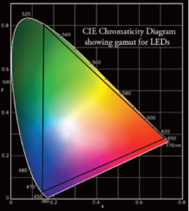
\includegraphics[width=0.5\linewidth]{images/Social Xray Triangle Basic.png}
    \caption{Chromatic triangle \cite{korff_junior_professor_interstitial_2015}}
    \label{fig:enter-label}
\end{figure}

Utilizing the Socio-Semantic X-Ray method, we test the propositions illustrated in Fig. \ref{fig:four-dynamics}: The Four Interstitial Patterns of Collaboration Between the Three Journals—(a) Differentiation, (b) Recombination, (c) Integration, and (d) Interstitial—following the conceptual framework proposed by \cite{Korff2015}. This integrative approach analyzes discursive (scientific) data, specifically full-text articles, alongside collaboration networks among the three journals (RSOG, EIST, and SUSSCI). By combining these two dimensions, we explore scientific discourse and cooperative dynamics in a multifaceted manner.

\paragraph{Methodological Approach:}
Our method integrates:
\begin{itemize}
    \item \textbf{Semantic Analysis of Full-Text Articles:} This aspect decodes the substantive content of scientific communication, uncovering the cultural codes and disciplinary lexicons that define knowledge within the studied domains. It enables the identification of distinct vocabularies, recurring themes, and emerging research areas.
    \item \textbf{Collaboration Network Mapping:} By analyzing co-authorship and institutional relationships, we chart the structural connections that bind researchers and institutions. This reveals the social architecture of scientific production and collaboration.
\end{itemize}

This synthesis provides a comprehensive perspective on how intellectual discourse and collaborative relationships co-evolve, influencing both the development of scientific fields and the dissemination of knowledge across the academic landscape. By visualizing relationships among authors based on their shared vocabulary and research topics, this technique offers a graphical representation of the discourse networks' interstitial nature.


\subsection{Integration of Semantic and Social Dimensions: Mapping Concepts (Topics and Methods) with Authors/Knowledge Producers}
The Socio-Semantic X-Ray method integrates two complementary dimensions of analysis: semantic analysis and social network analysis. These dimensions, when combined, provide a comprehensive view of knowledge production by linking the content of scientific literature to the collaborative structures underlying its creation and dissemination.

\begin{enumerate}
    \item \textbf{Semantic Analysis:} This dimension examines the thematic content of scientific literature, focusing on the identification of key topics, trends, and conceptual relationships. Using BERTopic modeling, the method uncovers latent themes, classifies articles, and tracks thematic evolution over time. This analysis maps the intellectual landscape of sustainability science, revealing both dominant themes and emerging areas of research.
    \item \textbf{Social Network Analysis:} This dimension explores collaboration patterns among authors and institutions, providing insights into network structures, key actors, and interstitial knowledge flows. By applying metrics such as centrality, modularity, and betweenness, the method identifies influential authors and those who serve as bridges between disconnected research communities.
\end{enumerate}

This dual-layered approach addresses significant limitations in traditional computational literature reviews, which often treat semantic content and social structures as separate domains. By integrating these perspectives, the Socio-Semantic X-Ray method enables a more holistic understanding of sustainability science’s knowledge ecosystem. For example, this approach allows us to map how specific research themes are distributed across collaborative networks, highlighting the interplay between intellectual production and social dynamics.

\paragraph{Hypotheses Testing:}
To test the four proposed collaboration dynamics (see Fig. \ref{fig:four-dynamics}), we hypothesize that:
\begin{enumerate}
    \item \textbf{Differentiation Dynamics:} Collaboration occurs within disciplinary silos, with minimal overlap in vocabulary and research themes (Fig. \ref{fig:diff-dynamics}).
    \item \textbf{Integration Dynamics:} Authors collectively align on common topics and vocabularies, representing cohesive interdisciplinary collaboration (Fig. \ref{fig:integ-dynamics}).
    \item \textbf{Recombination Dynamics:} Researchers selectively draw from different fields, combining distinct vocabularies to create new hybridized concepts (Fig. \ref{fig:recomb-dynamics}).
    \item \textbf{Interstitial Dynamics:} Few authors act as bridges, occupying interstitial spaces where they mediate knowledge exchange across distinct fields (Fig. \ref{fig:interstitial-dynamics}).
\end{enumerate}

We hypothesize that interstitial dynamics, represented by authors occupying these bridging positions, are rare but critical for enabling cross-disciplinary integration. By mapping discourse networks based on author vocabularies and collaboration patterns, we aim to validate these propositions and reveal the spatial distribution of discourse interstices.

\paragraph{Visualization of Patterns:}
The four proposed dynamics are visualized in Fig. \ref{fig:four-dynamics}, where:
\begin{itemize}
    \item Subfigure \ref{fig:diff-dynamics} illustrates collaboration dominated by disciplinary differentiation.
    \item Subfigure \ref{fig:integ-dynamics} highlights cohesive integration across disciplines.
    \item Subfigure \ref{fig:recomb-dynamics} shows hybridization through recombination of vocabularies.
    \item Subfigure \ref{fig:interstitial-dynamics} depicts the critical bridging roles within interstitial spaces.
\end{itemize}

\begin{figure}[ht]
    \centering
    \begin{subfigure}[b]{0.45\columnwidth}
        \centering
        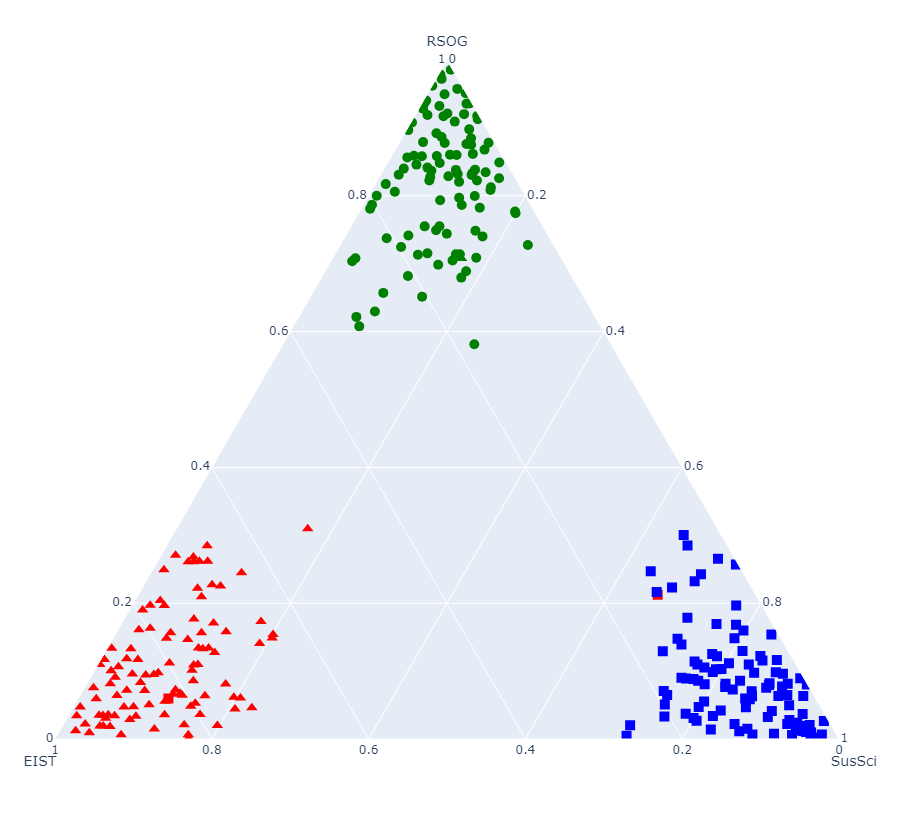
\includegraphics[width=\linewidth]{images/3j_diffsim.png}
        \caption{Differentiation Dynamics}
        \label{fig:diff-dynamics}
    \end{subfigure}
    \hfill
    \begin{subfigure}[b]{0.45\columnwidth}
        \centering
        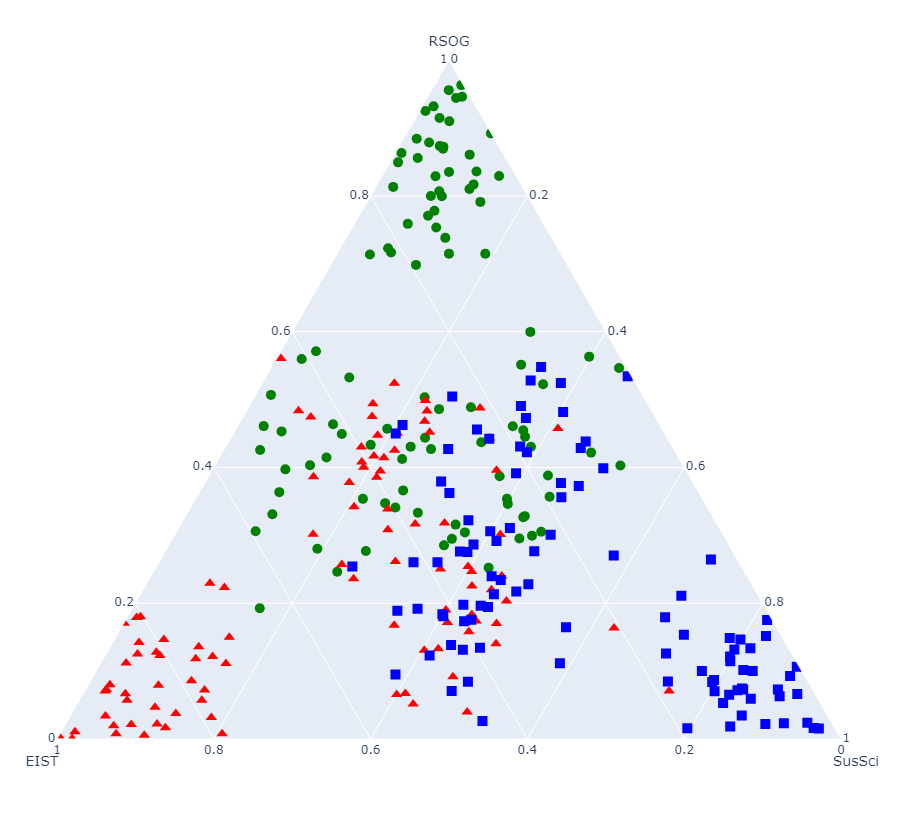
\includegraphics[width=\linewidth]{images/3j_intsim.png}
        \caption{Integration Dynamics}
        \label{fig:integ-dynamics}
    \end{subfigure}
    \vspace{1em}
    \begin{subfigure}[b]{0.45\columnwidth}
        \centering
        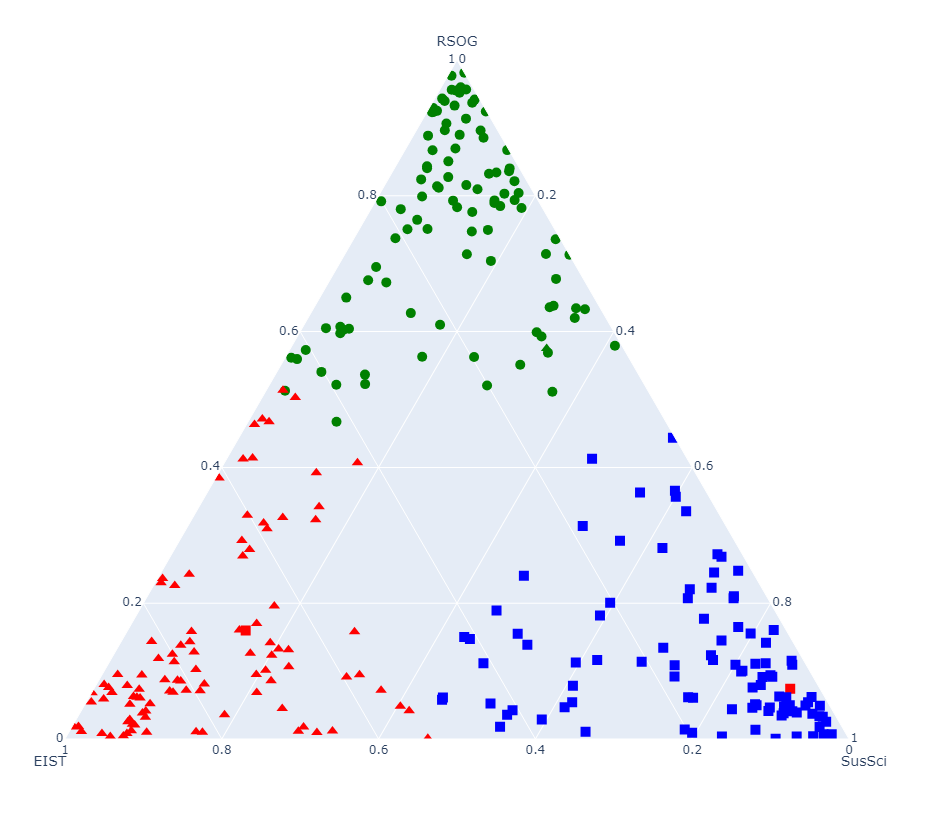
\includegraphics[width=\linewidth]{images/3j_recombsim.png}
        \caption{Recombination Dynamics}
        \label{fig:recomb-dynamics}
    \end{subfigure}
    \hfill
    \begin{subfigure}[b]{0.45\columnwidth}
        \centering
        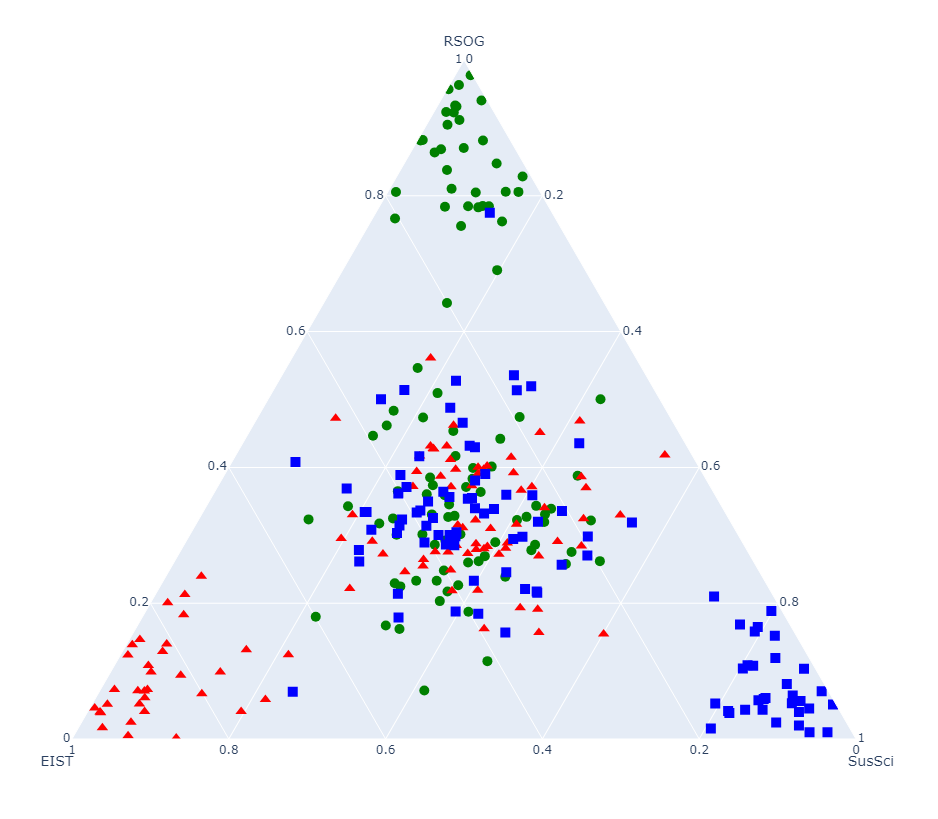
\includegraphics[width=\linewidth]{images/3j_interstitialsim.png}
        \caption{Interstitial Dynamics}
        \label{fig:interstitial-dynamics}
    \end{subfigure}
    \caption{The Four Dynamics Hypothesized: (a) Differentiation, (b) Integration, (c) Recombination, and (d) Interstitial Dynamics in the three journals.}
    \label{fig:four-dynamics}
\end{figure}

This synthesis, combining linguistic topography visualization and interstitial network mapping, provides a novel lens for understanding the dynamics of collaboration and discourse in sustainability science. By bridging semantic and social dimensions, we reveal how scientific discourse evolves across disciplinary boundaries.

\iffalse
\footnote{Socio-Institutional Theory in Transitions Research}
Socio-Institutional Theory provides a meta-theoretical lens for understanding large-scale societal change, emphasizing the interplay of technological, institutional, and social dimensions. This perspective informs the analysis of interstitial knowledge spaces, where authors mediate between distinct institutional and disciplinary domains. By mapping these spaces, the method highlights pathways for cross-disciplinary collaboration and innovation.\cite{loorbach_sustainability_2017}
\fi

\subsection{Conceptual Innovations}
The Socio-Semantic X-Ray method introduces several conceptual advancements that enhance our understanding of sustainability science:
\begin{itemize}
    \item \textbf{Interstitial Knowledge Mapping:} Identifying and visualizing authors who act as bridges between distinct research domains, thereby enabling interdisciplinary knowledge transfer.
    \item \textbf{Dual-Layered Analysis:} Integrating semantic and social analyses to provide a holistic view of knowledge production that captures both thematic trends and collaborative structures.
    \item \textbf{Dynamic Knowledge Networks:} Conceptualizing knowledge production as an evolving ecosystem shaped by continuous interactions between ideas, individuals, and institutions.
\end{itemize}

These innovations reposition computational literature reviews as active tools for knowledge mapping, moving beyond passive content extraction to uncover hidden patterns in interdisciplinary research\cite{antons_computational_2023}. By synthesizing theoretical perspectives and methodological approaches, the Socio-Semantic X-Ray method offers a robust framework for comprehensively analyzing scientific literature in sustainability science.


\subsubsection{Integrating Linguistic Topography and Relational Structures}

The Socio-Semantic X-Ray method integrates linguistic analysis and relational network mapping to identify interstitial dynamics within sustainability science. By examining authors' vocabularies and collaboration patterns, this approach uncovers interstitial zones where scientific discourse evolves, disciplinary boundaries are bridged, and interdisciplinary knowledge transfer occurs. 

\paragraph{Linguistic Topography}
Authors' vocabularies are mapped into a semantic space that reflects their alignment with three major domains represented by the journals: EIST (socio-technical transitions), SUSSCI (systems-based sustainability perspectives), and RSOG (institutional dynamics). This visualization identifies interstitial authors who blend vocabularies across domains, producing hybridized discourses. Inspired by the chromatic triangle model of Korff et al. (2015), this semantic space is constructed as follows:
\begin{itemize}
    \item Axis Definitions: Each axis corresponds to one of the three journals:
    \begin{enumerate}
        \item EIST (socio-technical transitions): Vocabulary focused on innovation, technology, and socio-technical systems.
        \item SUSSCI (systems-based sustainability): Terminology reflecting systemic approaches to ecological and environmental challenges.
        \item RSOG (institutional dynamics): Language centered on governance, organizational sociology, and institutional change.
    \end{enumerate}
    \item Positional Mapping: Authors are positioned within this triangular space based on the proportional use of terms associated with each journal. For example, an author with equal contributions to all three domains occupies a central interstitial position, while authors concentrated in one domain align near that axis.
\end{itemize}

This mapping reveals patterns of linguistic blending, allowing us to identify interstitial zones where authors mediate across journal domains by adopting and integrating diverse vocabularies.

\paragraph{Relational Structure}
Collaboration networks are overlaid onto the linguistic topography to chart the structural connections among authors and institutions. By combining these two layers, the Socio-Semantic X-Ray method provides insights into the interplay between discourse and collaboration. Key findings include:
\begin{itemize}
    \item Interstitial Zones: Areas where authors display both linguistic blending and dense relational connectivity, serving as critical bridges between disciplines.
    \item Disciplinary Silos: Clusters of authors who operate predominantly within a single journal domain, with minimal interdisciplinary connectivity.
\end{itemize}

This dual-layered analysis highlights how collaboration and discourse co-evolve, revealing the mechanisms through which knowledge transfer occurs across disciplinary boundaries.

\paragraph{Key Insights}
This integrative framework emphasizes the pivotal role of interstitial authors in shaping sustainability science. Specifically, these authors:
\begin{enumerate}
    \item Blend vocabularies from EIST, SUSSCI, and RSOG to create novel, hybrid discourses.
    \item Facilitate cross-disciplinary collaboration by connecting otherwise disconnected communities.
    \item Act as conversational bridges, recombining concepts to address multifaceted sustainability challenges.
\end{enumerate}

By visualizing the intersection of linguistic and relational dimensions, the Socio-Semantic X-Ray method uncovers interstitial dynamics critical to the development of interdisciplinary sustainability science.


\section{Methodology}
\label{sec:methodology}

This study employs a Computational Literature Review (CLR) combined with the Social-Xray method to analyze the interdisciplinary research landscape across three journals: Research in the Sociology of Organizations (RSOG), Environmental Innovation and Societal Transitions (EIST), and Sustainability Science (SUSSCI). Our approach integrates topic modeling, network analysis, and visualization to identify interstitial dynamics and the interplay between scientific discourse and collaboration.



\subsection{Socio Semantic -XRAY Process}
\label{sec:social_xray}

\subsubsection{Mapping Linguistic and Relational Structures}
The Social-Xray method integrated linguistic analysis with network mapping to uncover interstitial dynamics. Authors’ vocabularies were mapped onto a semantic space aligned with three domains: socio-technical transitions (EIST), sustainability science (SUSSCI), and organizational studies (RSOG). Collaboration networks were overlaid to identify:
\begin{itemize}
    \item Interstitial Zones: Areas where authors blend vocabularies and maintain connections across domains.
    \item Disciplinary Silos: Clusters of authors operating within a single domain.
\end{itemize}

This mapping revealed interstitial authors as pivotal nodes in facilitating cross-disciplinary collaboration and discourse.

\subsection{Data Visualization and Analysis}
Network visualizations were generated using Sigma.js for flexibility in layout and styling. These visualizations supported hypothesis testing and enabled the identification of patterns, such as topic overlaps and the temporal evolution of research trajectories. The integration of semantic and relational analyses provided insights into how scientific discourse and collaboration co-evolve across the three journals.

\subsection{Data and Code Availability}
The processed data and analysis pipelines, including topic modeling and network mapping code, are available as open-source resources to encourage reproducibility and further exploration. Outputs are stored in JSON and CSV formats for compatibility with various analytical tools.

This study introduces methodological innovations that integrate computational methods with advanced visualization and network analysis techniques. The Socio-Semantic X-Ray Toolkit, at the core of this research, enables the mapping of interstitial knowledge spaces through a combination of linguistic and relational analyses.

\subsection{X-Ray Toolkit Architecture}
The X-Ray Toolkit is designed as a modular system that integrates multiple computational methods into a unified workflow. The architecture comprises three main components:
\begin{itemize}
    \item \textbf{Data Acquisition and Preprocessing:} Automates the harvesting of full-text articles and metadata from selected journals and processes text data for computational analysis.
    \item \textbf{Topic Modeling and Embedding Generation:} Employs algorithms like LDA and BERTopic to extract latent topics and generate embeddings that represent linguistic structures in high-dimensional space.
    \item \textbf{Network Mapping and Visualization:} Leverages network analysis tools (e.g., Sigma.js) to create visualizations that integrate linguistic and relational dimensions, facilitating the identification of interstitial authors and topics.
\end{itemize}
This modular architecture supports flexibility, enabling integration with additional machine learning algorithms or domain-specific datasets as needed.

\begin{figure}
\centering
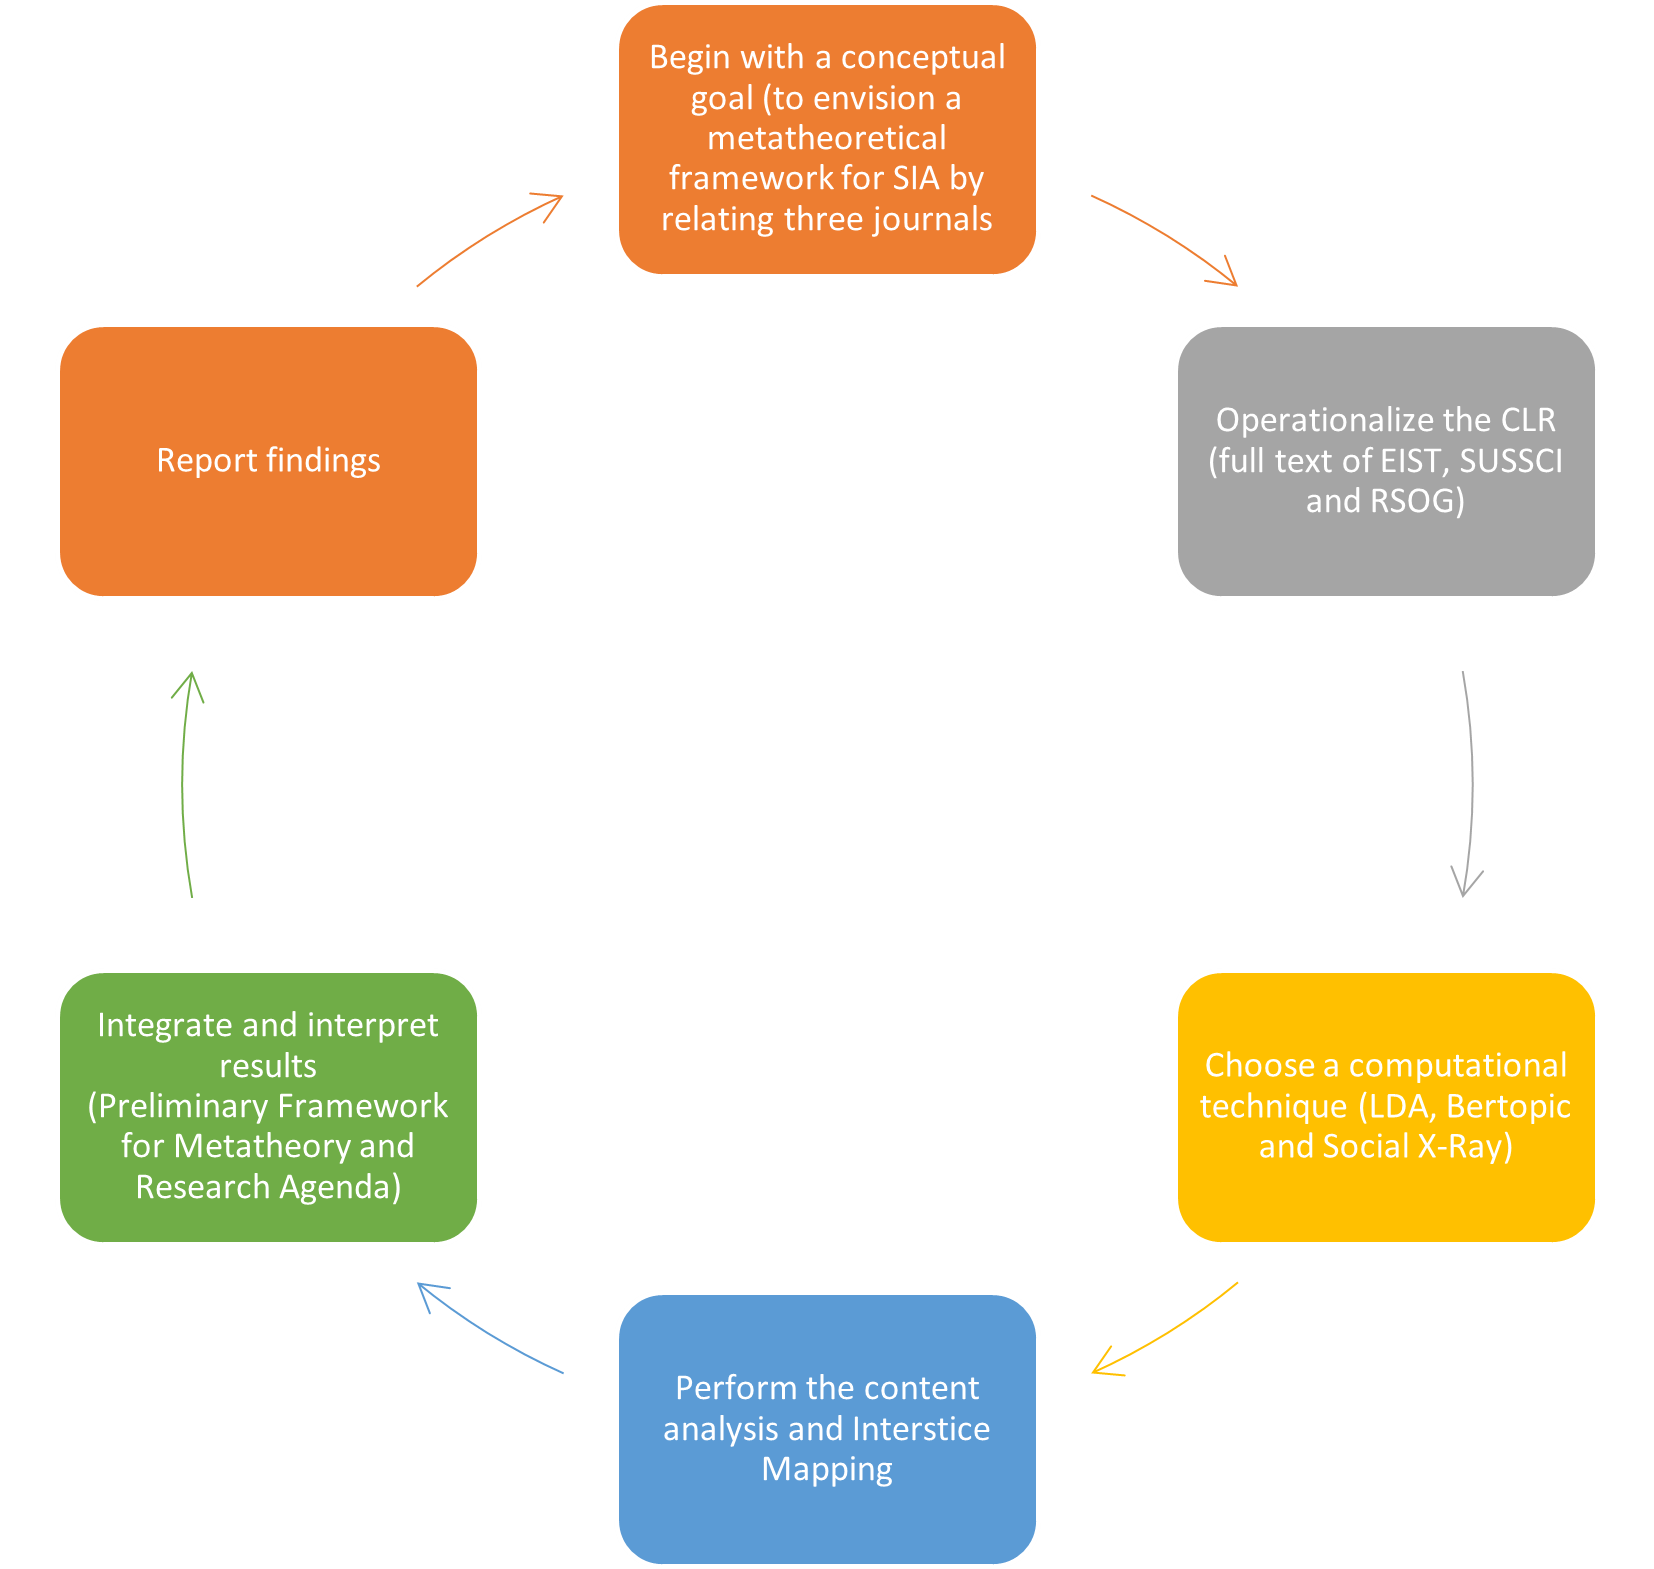
\includegraphics[width=0.6\columnwidth]{images/clr_xray_process.png} % Adjust the file name and path as needed.
\caption{CLR Social-Xray Hybrid Process for this paper based on \cite{Antons2023107} and \cite{Korff2015}.} 
\end{figure}

\subsection{Computational Methods Integration}
The methodology integrates multiple computational techniques into a cohesive framework:
\begin{itemize}
    \item Natural Language Processing (NLP): For preprocessing and linguistic analysis, including stemming, lemmatization, and vocabulary alignment across domains.
    \item Topic Modeling: Combines probabilistic (LDA) and neural-network-based (BERTopic) approaches to uncover latent themes and track their evolution.
    \item Network Analysis: Uses centrality measures, modularity, and community detection to analyze collaboration structures and their interplay with identified topics.
    \item Visualization: Adopts Sigma.js for interactive and customizable network visualizations, highlighting interstitial patterns.
\end{itemize}
By synthesizing these methods, the X-Ray Toolkit bridges semantic and social dimensions, offering a holistic approach to computational literature mapping.

\subsection{Data Processing Pipeline}
The data processing pipeline follows a structured workflow:
\begin{enumerate}
    \item \textbf{Data Collection:} Articles were sourced from RSOG, EIST, and SUSSCI using Web of Science and Scopus.
    \item \textbf{Text Preprocessing:} Steps include stop-word removal, lemmatization, punctuation elimination, and case normalization to ensure clean and consistent input data.
    \item \textbf{Topic Modeling and Embedding Generation:} LDA and BERTopic algorithms were applied, and coherence scores were used to validate topic quality.
    \item \textbf{Network Construction:} Co-authorship and keyword co-occurrence networks were generated, with additional metadata enriching the relational dataset.
    \item \textbf{Visualization and Analysis:} Network layouts and interstitial zones were visualized, enabling hypothesis testing and exploratory analysis.
\end{enumerate}
This pipeline ensures scalability and reproducibility, accommodating large datasets while maintaining methodological rigor.

%\subsection{Knowledge Management Implementation}
%The implementation focuses on leveraging computational methods to understand knowledge flows and interstitial dynamics across the three journals. By integrating topic modeling and network analysis, this approach enables insights into both content and collaboration.

\subsection{Multi-Journal Analysis Framework}
The selection of RSOG, EIST, and SUSSCI provides a comprehensive perspective on socio-institutional dynamics, environmental innovation, and sustainability science. The multi-journal framework emphasizes:
\begin{itemize}
    \item \textbf{Complementarity of Disciplines:} Each journal represents a unique perspective, contributing to a rich interdisciplinary dataset.
    \item \textbf{Unified Analytical Lens:} The integration of data from all three journals enables the identification of shared themes and divergent trends.
    \item \textbf{Temporal Analysis:} Examines the evolution of topics and collaboration patterns over time, providing insights into emerging research areas.
\end{itemize}

\subsection{Topic Modeling Process}
\textbf{Latent Dirichlet Allocation (LDA):} Identifies latent topics based on word distributions across documents. It is particularly suited for mapping general themes within the dataset.

\begin{figure}[ht]
    \centering
    % Top left image
    \begin{subfigure}[b]{0.45\columnwidth}
        \centering
        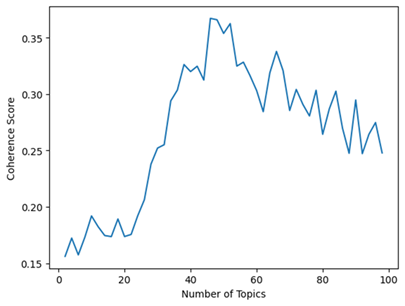
\includegraphics[width=\linewidth]{images/lda_eist.png}
        \caption{Comparison of Different Models’ Predictive Likelihood for EIST (n=40)}
        \label{fig:eist}
    \end{subfigure}
    \hfill % Space between the top two images
    % Top right image
    \begin{subfigure}[b]{0.45\columnwidth}
        \centering
        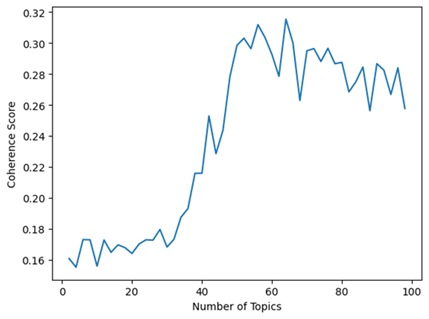
\includegraphics[width=\linewidth]{images/lda_sussci.png}
        \caption{Comparison of Different Models’ Predictive Likelihood for SUSSCI (n=66)}
        \label{fig:sussci}
    \end{subfigure}

    \vspace{1em} % Space between the top and bottom rows

    % Bottom left image
    \begin{subfigure}[b]{0.45\columnwidth}
        \centering
        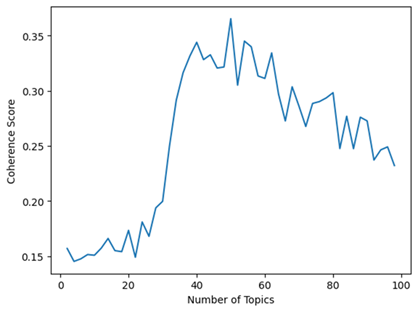
\includegraphics[width=\linewidth]{images/lda_rsog.png}
        \caption{Comparison of Different Models’ Predictive Likelihood for RSOG (n=50)}
        \label{fig:rsog}
    \end{subfigure}
    \hfill % Space between the bottom two images
    % Bottom right image
    \begin{subfigure}[b]{0.45\columnwidth}
        \centering
        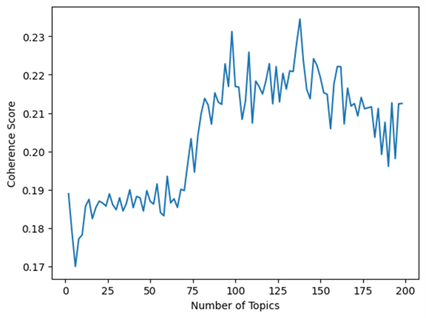
\includegraphics[width=\linewidth]{images/lda_3j.png}
        \caption{Comparison of Different Models’ Predictive Likelihood for Combined Corpus (n=138)}
        \label{fig:combined}
    \end{subfigure}

    % Overall caption for the figure
    \caption{Comparative Analysis of Different Models' Predictive Likelihood across Different Corpora}
    \label{fig:models-comparison}
\end{figure}

\textbf{BERTopic:} Provides refined, neural-embedding-based topic modeling, allowing for the detection of nuanced themes and subtopics. BERTopic outputs were validated using coherence scores and expert review.

\subsection{Interstitial Knowledge Detection}
\textbf{Linguistic and Relational Analysis:} By mapping authors' vocabularies and collaboration networks, the study identifies interstitial zones where distinct research domains intersect. These zones are crucial for cross-disciplinary innovation and knowledge transfer.

\textbf{Visualization of Interstitial Patterns:} Network visualizations highlight:
\begin{itemize}
    \item \textbf{Bridging Authors:} Individuals who mediate between distinct research communities.
    \item \textbf{Topic Overlaps:} Areas where themes from RSOG, EIST, and SUSSCI converge, forming interstitial knowledge spaces.
\end{itemize}

\textbf{Key Findings:} Interstitial authors are not only linguistically versatile but also occupy structurally significant positions within collaboration networks. Their role is pivotal in fostering interdisciplinary dialogue and advancing sustainability transitions research.


\section{Results \& Validation}



\begin{figure}[ht]
    \centering

    % First row of images
    \begin{subfigure}[b]{0.7\columnwidth}
        \centering
        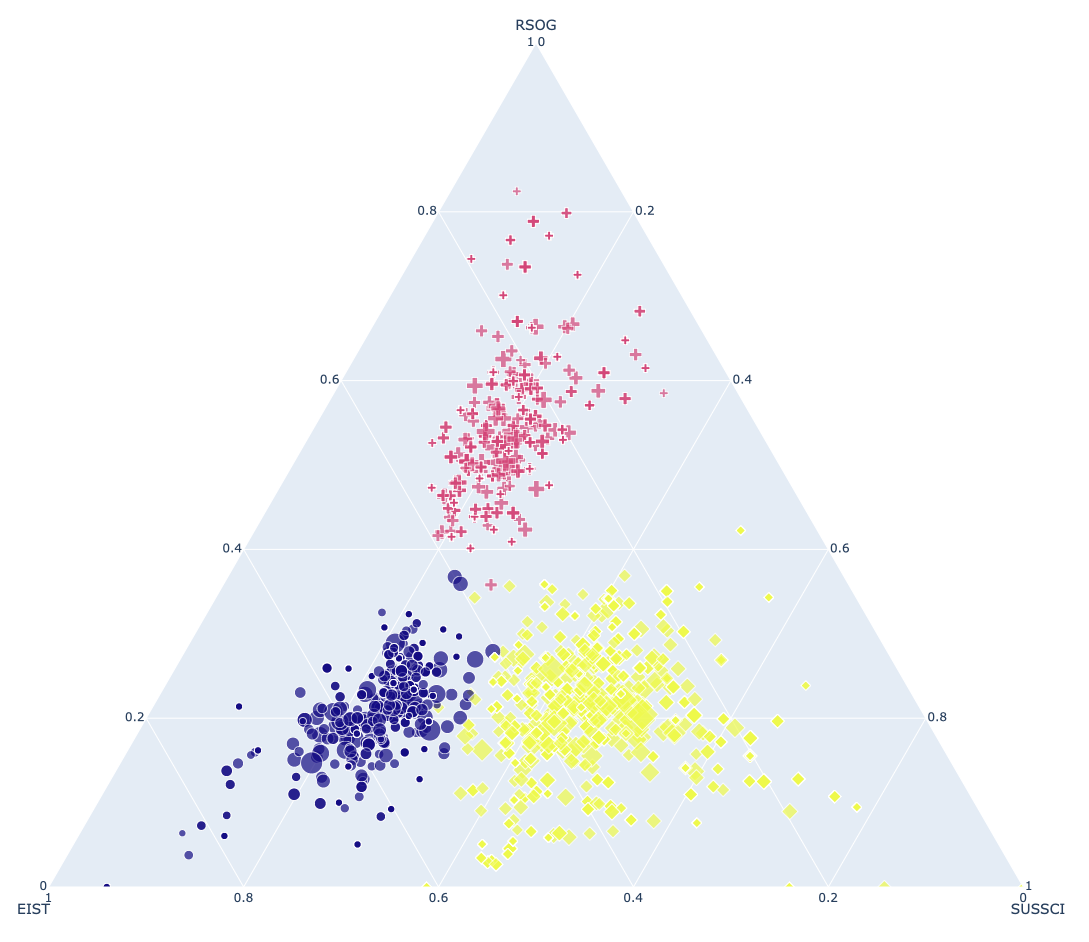
\includegraphics[width=\linewidth]{images/author_discourse.png}
        \caption{Discourse positions of authors from the three journals on a ternary plane.}
        \label{fig:pic1}
    \end{subfigure}
    \hfill % Space between two images in the same row
    \begin{subfigure}[b]{0.7\columnwidth}
        \centering
        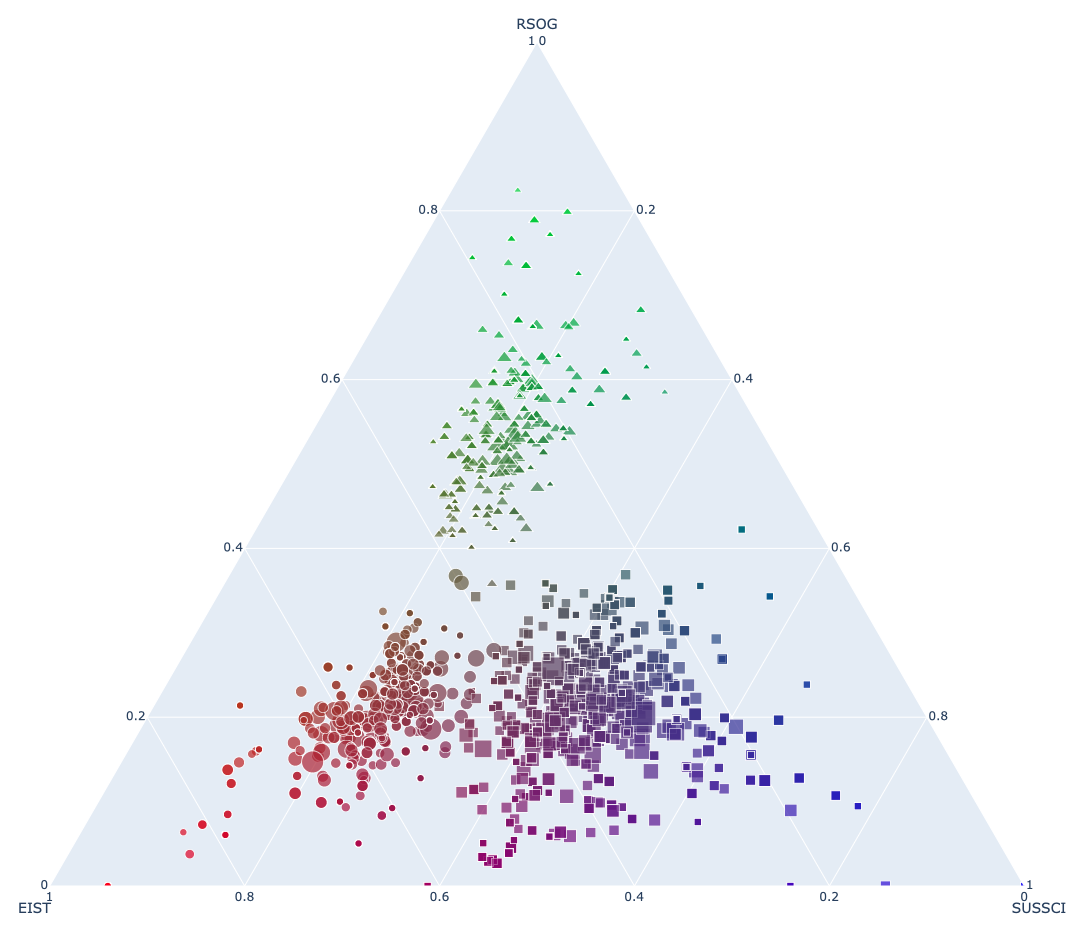
\includegraphics[width=\linewidth]{images/discourse_shift.png}
        \caption{Discourse positions with color intensity indicating the proportion of discourse shift.}
        \label{fig:pic3}
    \end{subfigure}

    % Overall caption for the figure
    \caption{Discourse positions of authors visualized on a 2D ternary plane. A vocabulary for each journal (RSOG, EIST, and SUSSCI) was created using topic-specific keywords derived from representative words and articles. These vocabularies were mapped to individual authors to define each author's discourse profile. The final position of each author on the plane reflects the proportion of their vocabulary associated with each journal. Node size represents both the number of articles authored and the strength of their vocabulary contributions.}
    \label{fig:ternary_discourse_plots}
\end{figure}

\subsection{Knowledge Structure Visualization}
\begin{figure}
    \centering
    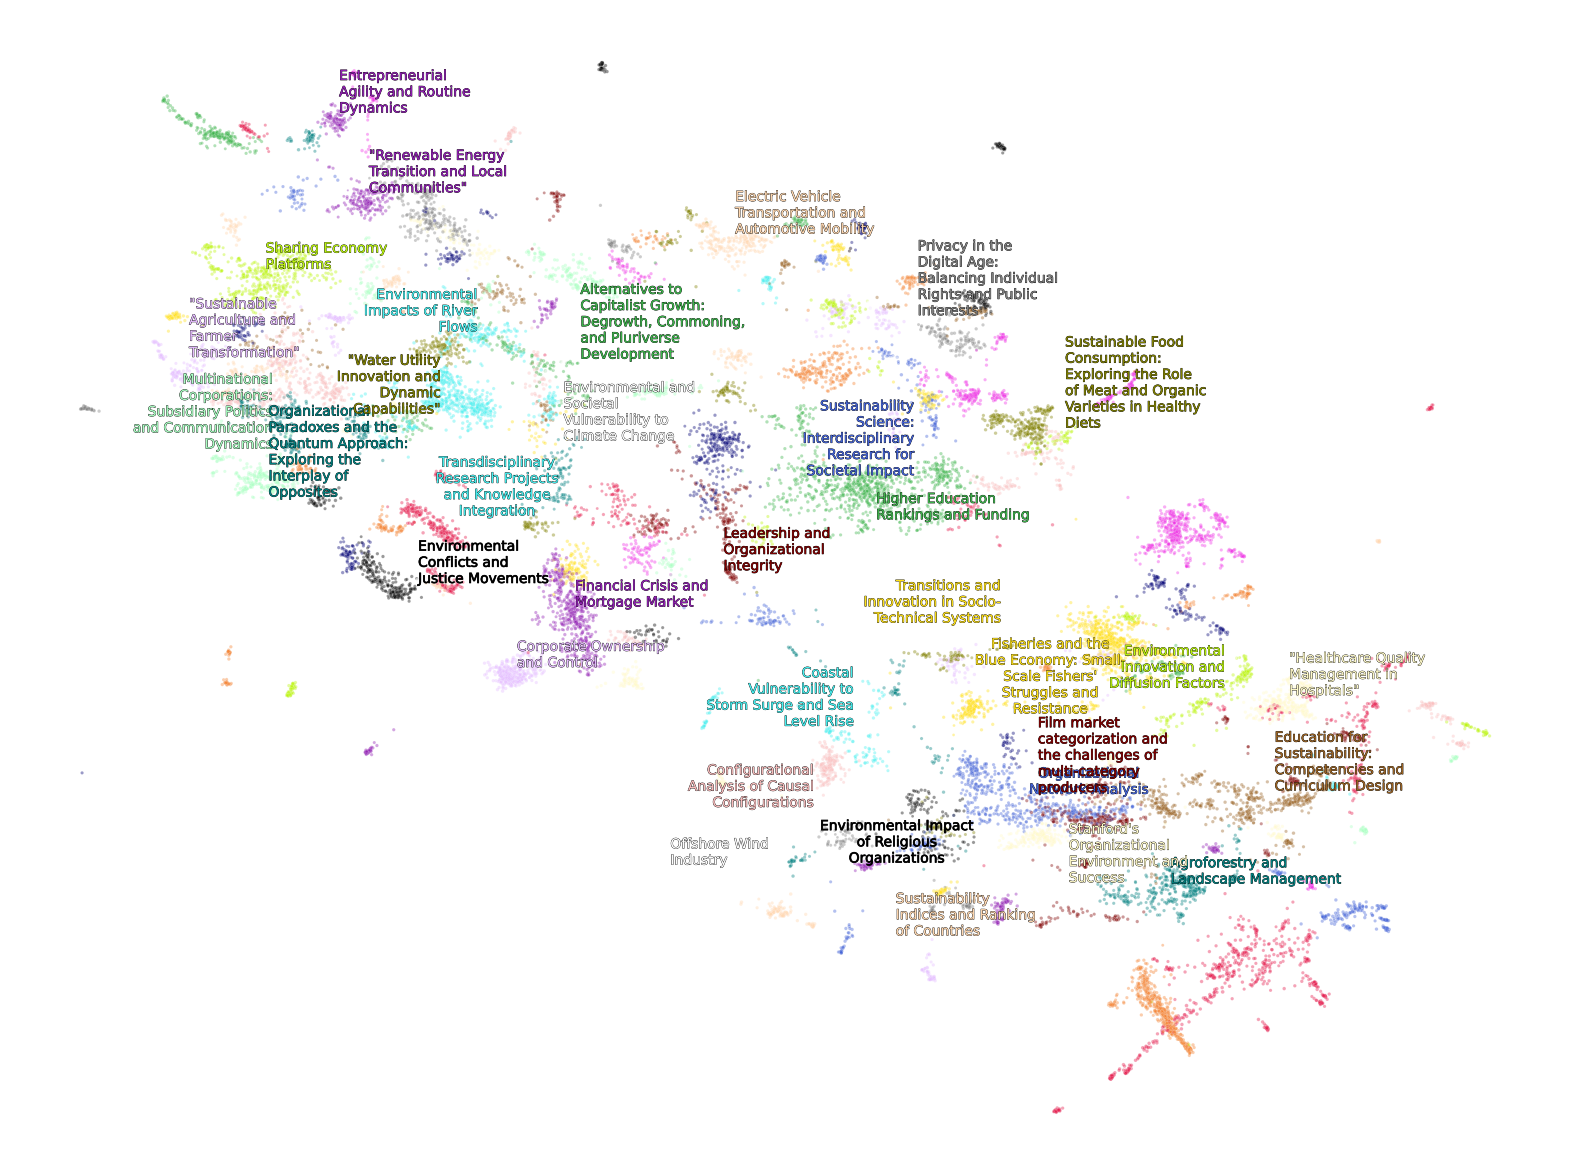
\includegraphics[width=1\linewidth]{images/all_tsne.png}
    \caption{Three Journals TSNE}
    \label{fig:enter-label}
\end{figure}
\begin{figure}
    \centering
    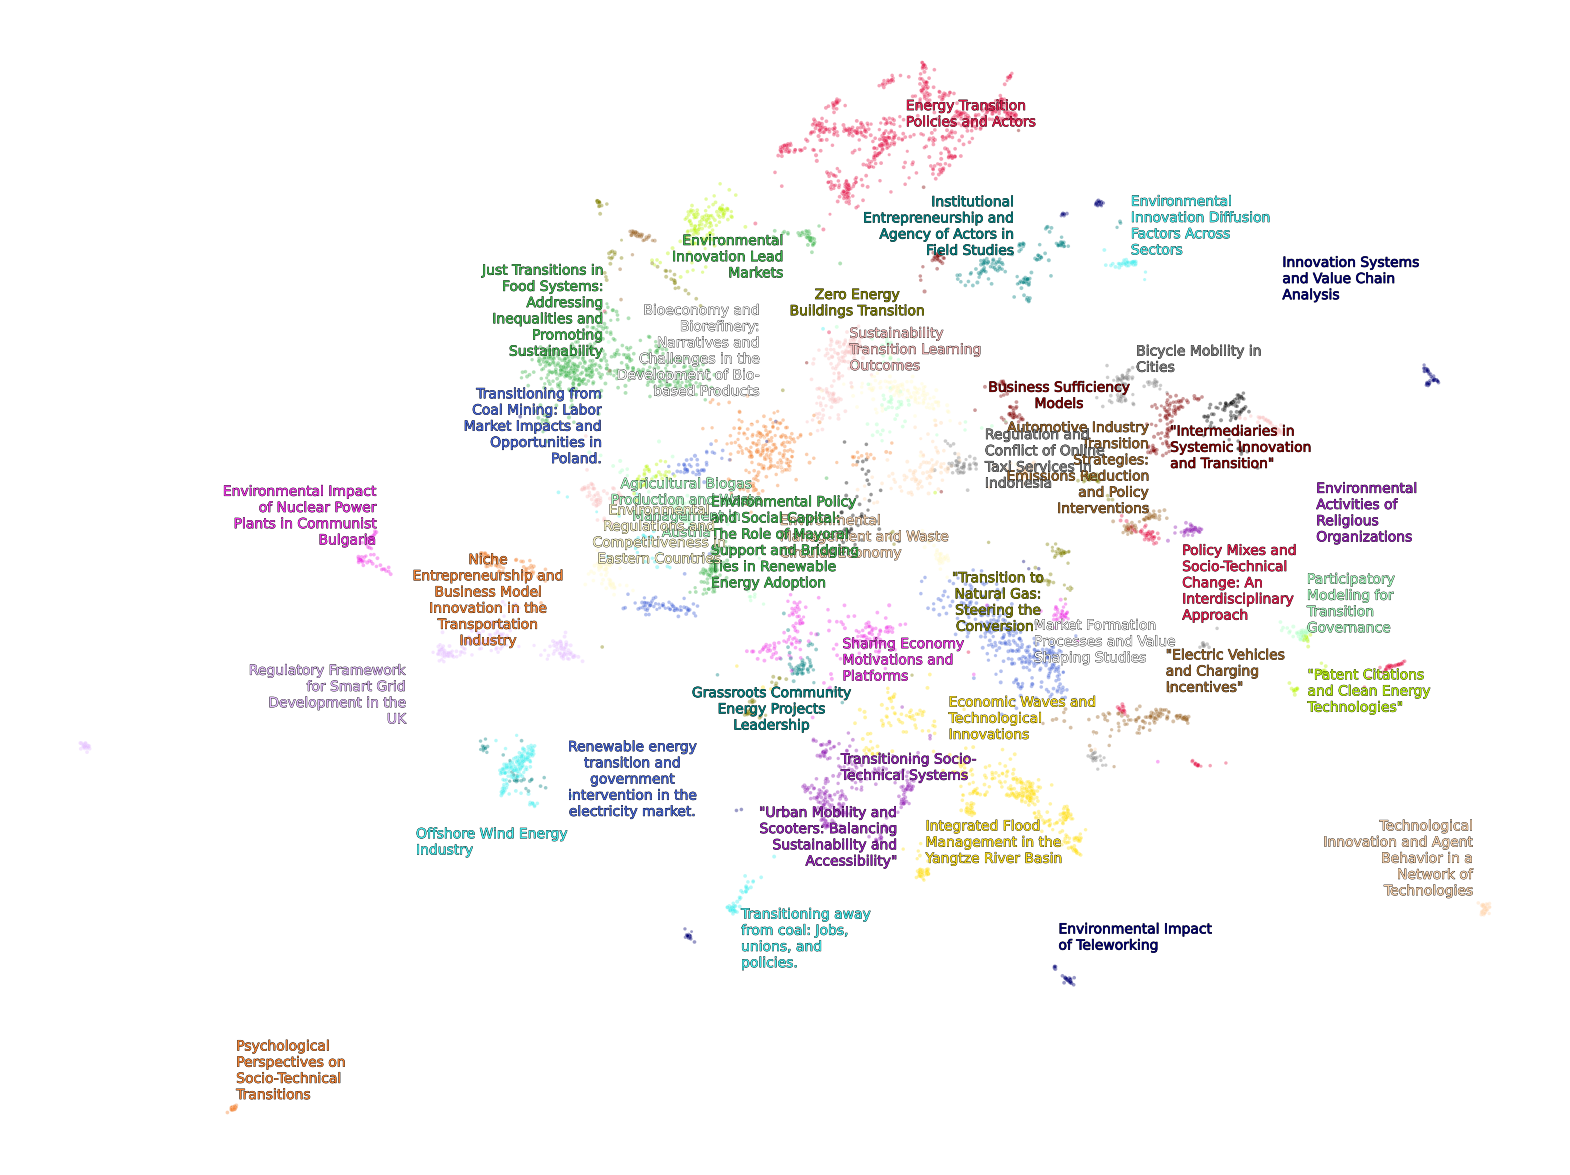
\includegraphics[width=1\linewidth]{images/eist_tsne.png}
    \caption{EIST Journal TSNE}
    \label{fig:enter-label}
\end{figure}
\begin{figure}
    \centering
    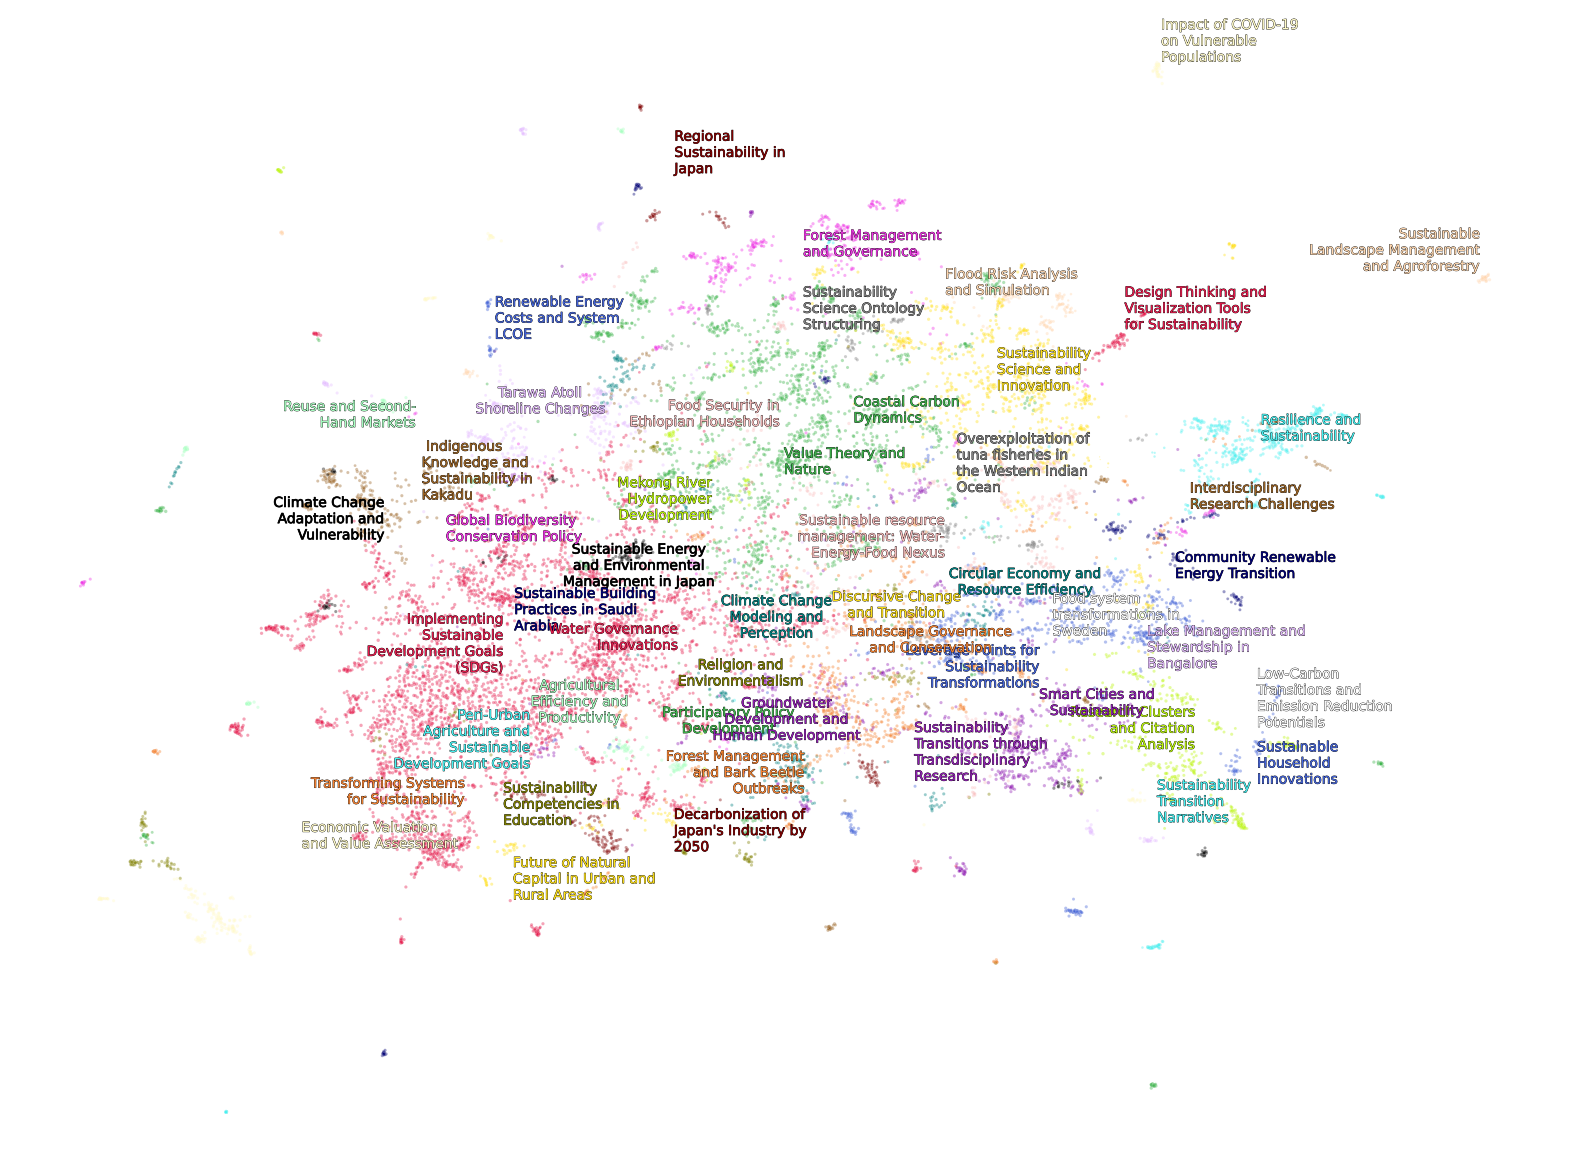
\includegraphics[width=1\linewidth]{images/sussci_tsne.png}
    \caption{SUSSCI Journal TSNE}
    \label{fig:enter-label}
\end{figure}
\begin{figure}
    \centering
    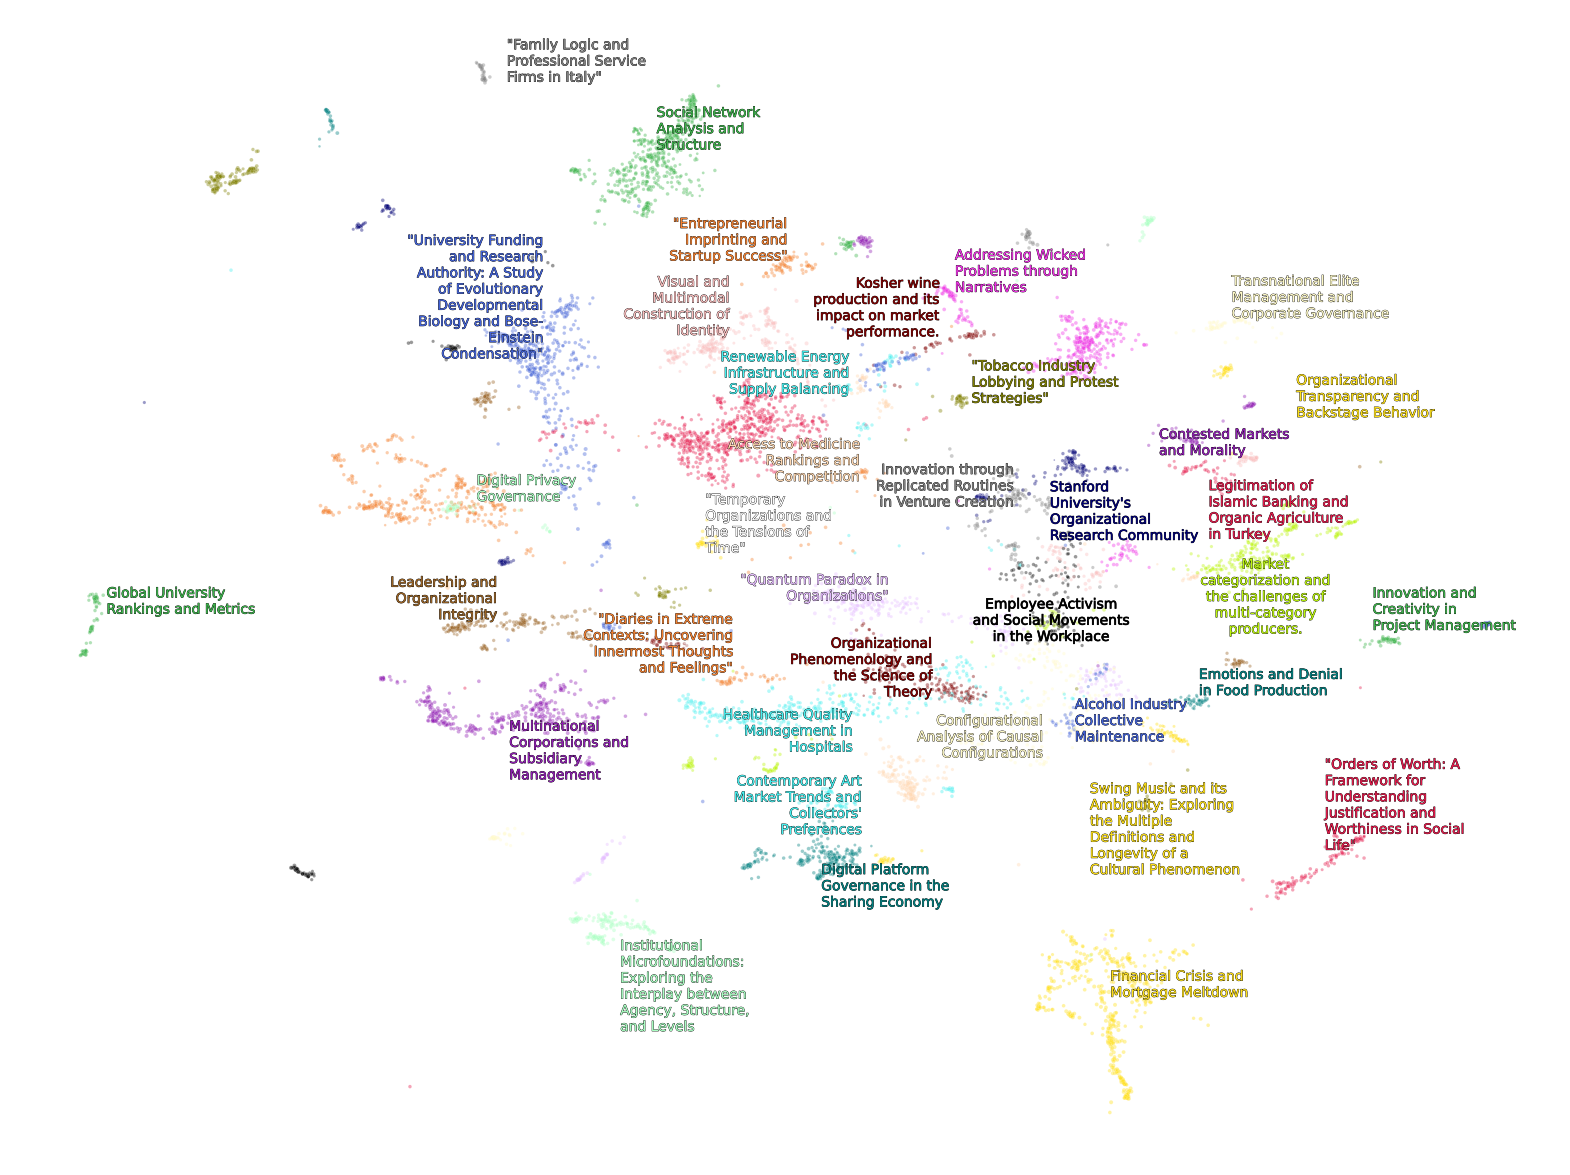
\includegraphics[width=1\linewidth]{images/rsog_tsne.png}
    \caption{RSOG Journal TSNE}
    \label{fig:enter-label}
\end{figure}
\begin{figure}[ht]
    \centering
    % Second row of images
    \begin{subfigure}[b]{0.7\columnwidth}
        \centering
        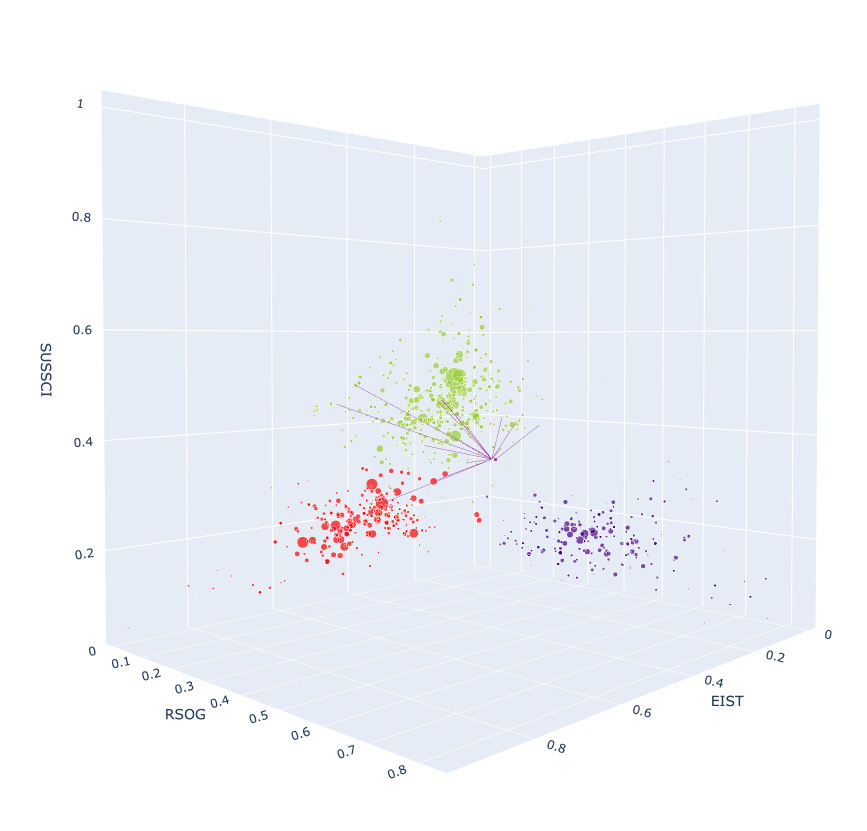
\includegraphics[width=\linewidth]{images/interstitial_colab.png}
        \caption{3D plot illustrating collaborations between interstitial authors and authors from the three journals.}
        \label{fig:pic2}
    \end{subfigure}
    \hfill
    \begin{subfigure}[b]{0.7\columnwidth}
        \centering
        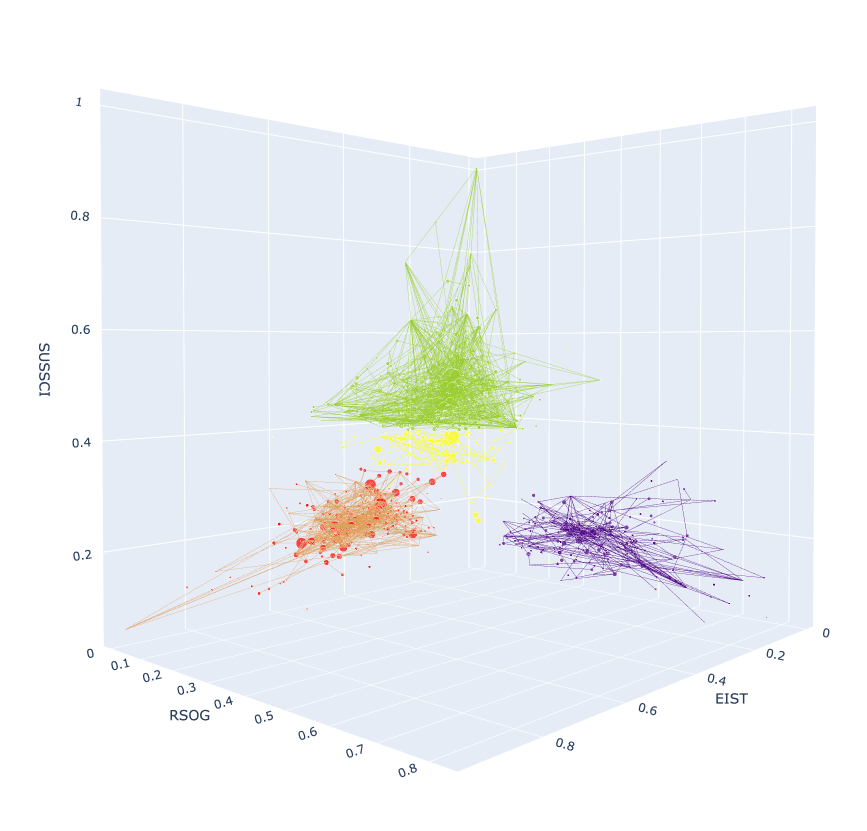
\includegraphics[width=\linewidth]{images/new_disocourse.png}
        \caption{3D plot highlighting newly identified discourse at the interstice of the three journals (yellow nodes) and collaborations within these groups.}
        \label{fig:pic4}
    \end{subfigure}

    \vspace{1em} % Space between rows

    % Third row of images
    \begin{subfigure}[b]{0.7\columnwidth}
        \centering
        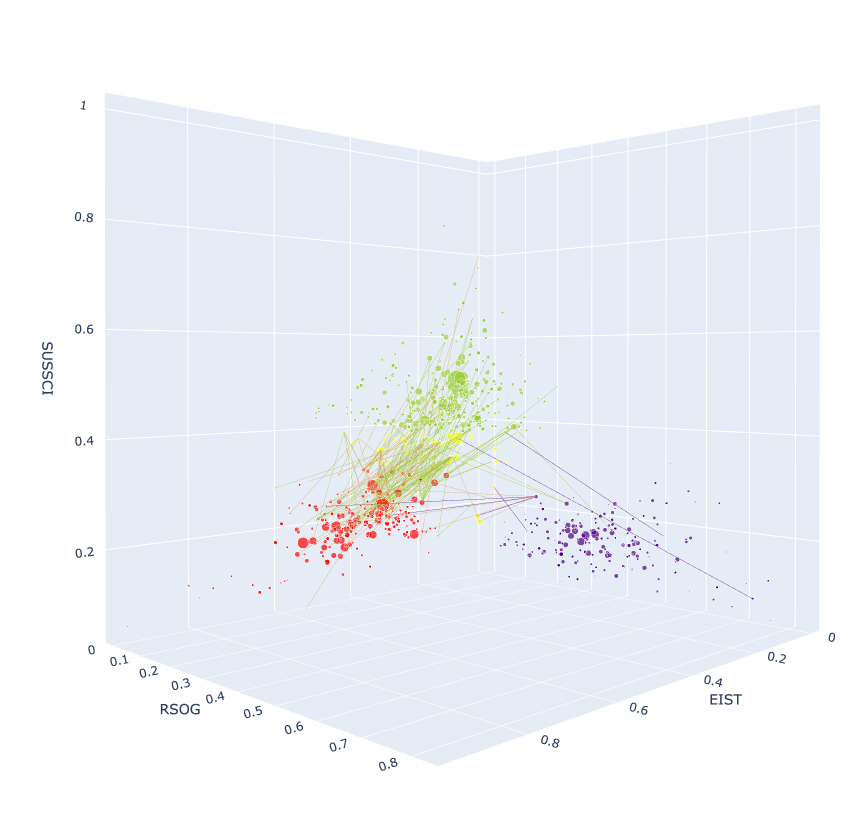
\includegraphics[width=\linewidth]{images/inter_journal_colab.png}
        \caption{3D plot visualizing inter-journal collaborations between authors.}
        \label{fig:pic5}
    \end{subfigure}
    \hfill
    \begin{subfigure}[b]{0.7\columnwidth}
        \centering
        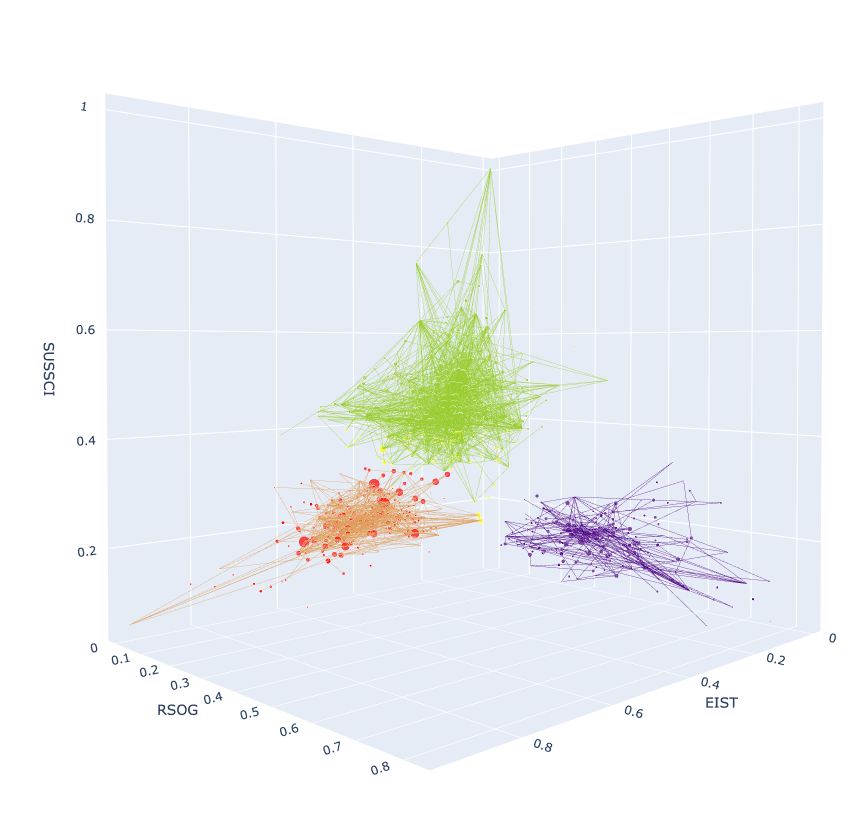
\includegraphics[width=\linewidth]{images/intra_journal_colab.png}
        \caption{3D plot visualizing intra-journal collaborations within each journal.}
        \label{fig:pic6}
    \end{subfigure}

    % Overall caption for the figure
    \caption{Visualization of discourse positions and collaboration patterns of authors in a 3D space. Discourse positions are calculated by creating a vocabulary for each journal (RSOG, EIST, and SUSSCI) using topic-specific representative words and articles. These vocabularies are mapped to individual authors to determine their discourse profiles. The final positions reflect the proportion of each author's vocabulary associated with the three journals. Node sizes correspond to the number of articles authored and the strength of their vocabulary contributions. The 3D plots highlight interstitial dynamics, newly identified discourses, and both inter- and intra-journal collaboration patterns.}
    \label{fig:3d_discourse_plots}
\end{figure}


\subsection{CLR Results - Identification of 138 Research Topics and Topic Networks}
\label{sec:research_topic_networks}
For topic node and edge definitions we follow Antons et al 2021. In the topic network, each of the 138 topics identified serves as a node. Edges between these nodes were established based on co-occurrence in individual articles, with a topic loading above the 10\% threshold, as recommended by Antons et al. (2016). For network measures, We calculated conventional network measures such as network density, node degree, and betweenness centrality using \hyperlink{Gephi}{https://gephi.org/} and \hyperlink{Sigma.js}{https://www.sigmajs.org/}. 

\begin{landscape}
\begin{figure}[htbp]
  \centering
  % Left half of the legend
  \begin{minipage}{0.25\textwidth}
    \tiny % Adjust the font size as necessary
    \begin{tabular}{rl}
      \toprule
      Topic Number & Topic Label \\
      \midrule
      0 &               interview\_data\_conducted\_participant \\
            1 &                 university\_student\_school\_stanford \\
            2 &                 complexity\_system\_approach\_process \\
            3 &            sustainability\_research\_student\_science \\
            4 &                           area\_land\_water\_scenario \\
            5 &             transformation\_actor\_change\_transition \\
            6 &                    transition\_energy\_policy\_carbon \\
            7 &           theory\_organization\_institutional\_volume \\
            8 &                            island\_area\_coast\_beach \\
            9 &                 emission\_scenario\_reduction\_carbon \\
           10 &                       japan\_scenario\_emission\_cost \\
           11 &                     diet\_scenario\_food\_consumption \\
           12 &             logic\_institutional\_field\_organization \\
           13 &                      biofuels\_fuel\_ethanol\_biofuel \\
           14 &                       water\_scenario\_area\_rainfall \\
           15 &                 forest\_land\_scenario\_deforestation \\
           16 &                         rice\_crop\_yield\_production \\
           17 &                             vehicle\_battery\_car\_ev \\
           18 &                 religion\_religious\_church\_practice \\
           19 &                       synergy\_sdgs\_trade offs\_offs \\
           20 &            transition\_innovation\_technology\_market \\
           21 &                        community\_village\_land\_year \\
           22 &                      transition\_city\_actor\_process \\
           23 &                       paradox\_theory\_logic\_tension \\
           24 &                       practice\_object\_logic\_theory \\
           25 &             shareholder\_corporation\_firm\_ownership \\
           26 &                hospital\_patient\_nurse\_professional \\
           27 &                          variable\_model\_error\_test \\
           28 &                          sdgs\_sdg\_target\_indicator \\
           29 &                      system\_approach\_science\_human \\
           30 &               transition\_political\_politics\_policy \\
           31 &                   actor\_institution\_process\_theory \\
           32 &                        process\_theory\_actor\_action \\
           33 &                    disaster\_hazard\_earthquake\_risk \\
           34 &                          mortgage\_bank\_loan\_market \\
           35 &           science\_knowledge\_process\_sustainability \\
           36 &                      ecological\_scale\_system\_human \\
           37 &                            wind\_energy\_power\_solar \\
           38 &                          crop\_land\_production\_area \\
           39 &                        fishery\_fisher\_growth\_ocean \\
           40 &       science\_discipline\_sustainability\_university \\
           41 &            interview\_interviewee\_snowball\_sampling \\
           42 &                    process\_system\_technology\_actor \\
           43 &                    consumer\_student\_market\_product \\
           44 &                        solar\_energy\_grid\_renewable \\
           45 &             church\_religion\_organization\_religious \\
           46 &                            god\_love\_religion\_world \\
           47 &                        artist\_song\_music\_recording \\
           48 &                          bike\_bicycle\_city\_cycling \\
           49 &                            worker\_white\_whig\_state \\
           50 &                        labor\_worker\_union\_platform \\
           51 &                    farmer\_sinaloa\_production\_maize \\
           52 &                actor\_identity\_institutional\_theory \\
           53 &                   paris\_agreement\_emission\_climate \\
           54 &         transition\_innovation\_framework\_literature \\
           55 &                logic\_organization\_identity\_process \\
           56 &                     ecological\_social\_human\_change \\
           57 &                  stakeholder\_project\_process\_level \\
           58 &              capitalist\_world\_colonialism\_colonial \\
           59 &                   qca\_condition\_configuration\_case \\
           60 &                       forest\_farmer\_land\_landscape \\
           61 &                 cost\_technology\_electricity\_energy \\
           62 &                     configuration\_qca\_outcome\_case \\
           63 & entrepreneur\_organizational\_entrepreneurship\_in... \\
           64 &                 category\_audience\_analyst\_identity \\
           65 &                 stanford\_school\_student\_university \\
           66 &                change\_climate\_ecological\_ecosystem \\
           67 &              organization\_theory\_process\_structure \\
           68 &                            island\_atoll\_area\_coast \\
      \bottomrule
    \end{tabular}
  \end{minipage}
  % The network plot
  \begin{minipage}{0.5\textwidth}
    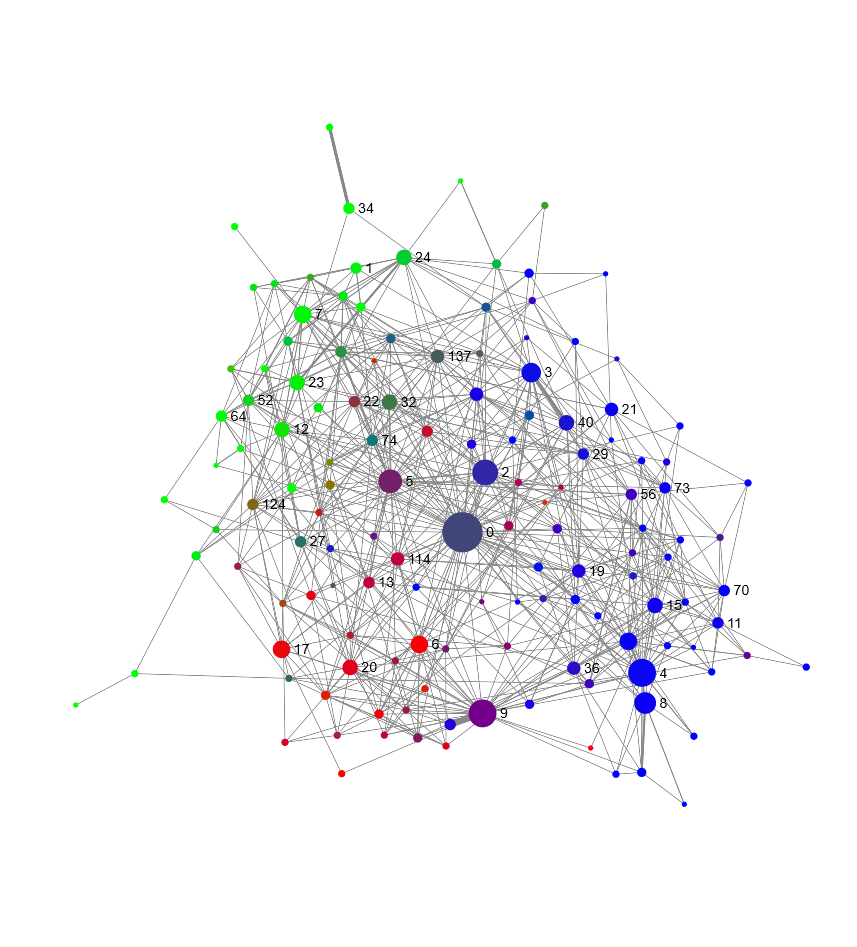
\includegraphics[width=\textwidth]{images/network_plots/3j.png}
  \end{minipage}
  % Right half of the legend
  \begin{minipage}{0.15\textwidth}
    \tiny % Adjust the font size as necessary
    \begin{tabular}{rl}
      \toprule
      Topic Number & Topic Label \\
      \midrule
      69 &               multimodal\_visual\_mode\_multimodality \\
           70 &                           farmer\_food\_crop\_farming \\
           71 &                         city\_urban\_experiment\_myth \\
           72 &                     synergy\_target\_sdgs\_trade offs \\
           73 &                    group\_community\_resource\_change \\
           74 &             behavior\_decision\_theory\_psychological \\
           75 &            researcher\_university\_research\_academic \\
           76 &                     interview\_data\_coding\_analysis \\
           77 &              race\_racial\_discrimination\_inequality \\
           78 &                     food\_transition\_agri food\_agri \\
           79 &     sustainability\_change\_transition\_environmental \\
           80 &                      mortgage\_meltdown\_crisis\_loan \\
           81 &                nature\_biodiversity\_ecosystem\_human \\
           82 &                      practice\_logic\_meaning\_action \\
           83 &                       disease\_farm\_pathogen\_farmer \\
           84 &               case\_theory\_research\_transferability \\
           85 &               bioeconomy\_bio\_biorefineries\_zealand \\
           86 &            transition\_policy\_technology\_innovation \\
           87 &            interview\_snowball\_sampling\_interviewee \\
           88 &               energy\_nuclear\_coalition\_electricity \\
           89 &                      car\_vehicle\_transport\_sharing \\
           90 &              landscape\_ecosystem\_biodiversity\_tree \\
           91 &                   process\_actor\_conflict\_knowledge \\
           92 &            science\_research\_sustainability\_problem \\
           93 &                    water\_management\_basin\_decision \\
           94 &                       meaning\_actor\_discourse\_form \\
           95 &                    africa\_african\_barometer\_malawi \\
           96 &                        water\_resource\_country\_year \\
           97 &    transformation\_sustainability\_transition\_change \\
           98 &                     process\_system\_place\_knowledge \\
           99 &                           marine\_tourism\_island\_rc \\
          100 &                    process\_system\_innovation\_actor \\
          101 &                       island\_port\_adaptation\_atoll \\
          102 &                tree\_forest\_landscape\_deforestation \\
          103 &                      bias\_sample\_survey\_respondent \\
          104 &                   technology\_industry\_module\_solar \\
          105 &                              farm\_farmer\_land\_crop \\
          106 &                    nature\_value\_concept\_relational \\
          107 &                   fishery\_fisher\_bay\_co management \\
          108 &                         company\_cost\_grid\_industry \\
          109 &                     carbon\_emission\_low\_technology \\
          110 &                     airline\_aircraft\_atp\_shipowner \\
          111 &                    city\_urban\_community\_transition \\
          112 &                     actor\_role\_perspective\_process \\
          113 &               community\_system\_approach\_management \\
          114 &                transition\_innovation\_energy\_policy \\
          115 &             problem\_future\_solution\_sustainability \\
          116 &                          impact\_design\_case\_output \\
          117 &                       japan\_capital\_prefecture\_iwi \\
          118 &                    dialogue\_discourse\_actor\_debate \\
          119 &                           storm\_cyclone\_sheet\_wind \\
          120 &                  external\_firm\_externality\_company \\
          121 &                      firm\_clique\_membership\_member \\
          122 &                organization\_external\_firm\_resource \\
          123 &              vulnerability\_climate\_change\_exposure \\
          124 &                       process\_context\_change\_niche \\
          125 &                  actor\_routine\_action\_acceleration \\
          126 &                organization\_individual\_form\_action \\
          127 &                              crop\_area\_forest\_land \\
          128 &                          delta\_sediment\_basin\_area \\
          129 &                system\_market\_technology\_transition \\
          130 &               technology\_transition\_country\_market \\
          131 &                  waste\_material\_recycling\_landfill \\
          132 &                transition\_system\_market\_technology \\
          133 &                     actor\_organization\_logic\_field \\
          134 &                     city\_urban\_environment\_ri city \\
          135 &                    variable\_model\_score\_regression \\
          136 &                       woman\_child\_family\_migration \\
          137 &                       game\_approach\_process\_change \\
      \bottomrule
    \end{tabular}
  \end{minipage}
  \caption{Three Journal Network plot with accompanying legend, Green-RSOG, Red-EIST, Blue-SUSSCI}
  \label{fig:3j_network_plot_with_legend}
\end{figure}
\end{landscape}

\begin{figure}[ht]
    \centering

    % First row of images
    \begin{subfigure}[b]{0.7\columnwidth}
        \centering
        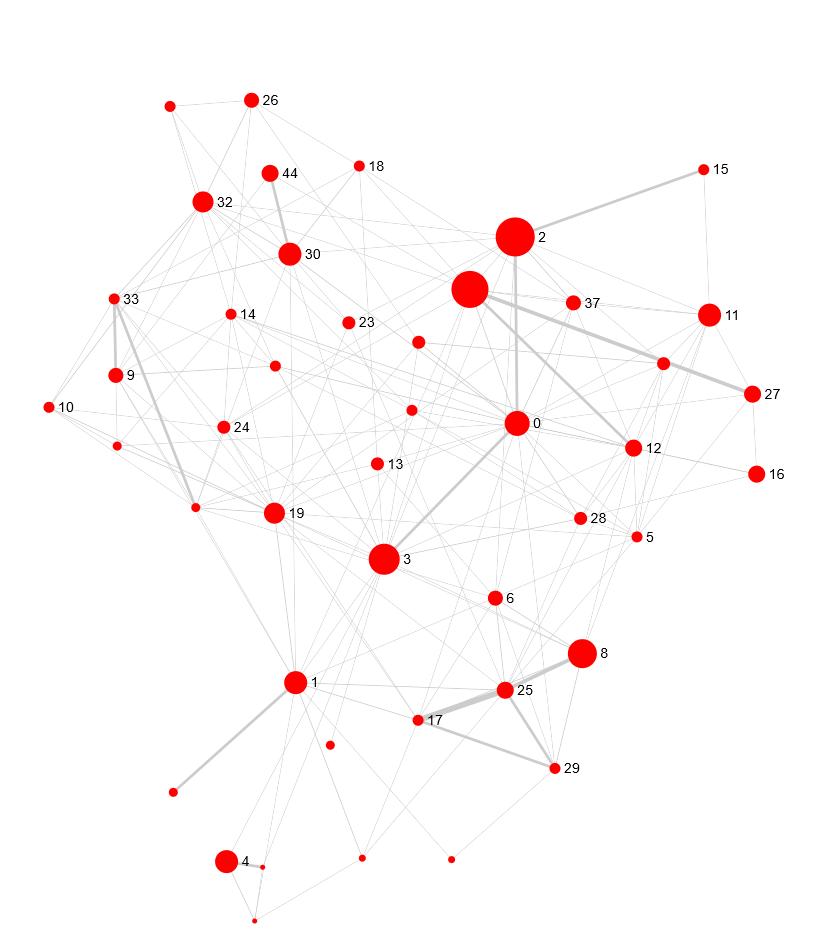
\includegraphics[width=\linewidth]{images/network_plots/eist_c.png}
        \caption{Topic network of EIST Journal}
        \label{fig:eist_topic_network}
    \end{subfigure}
    \hfill % Space between two images in the same row
    \begin{subfigure}[b]{0.7\columnwidth}
        \centering
        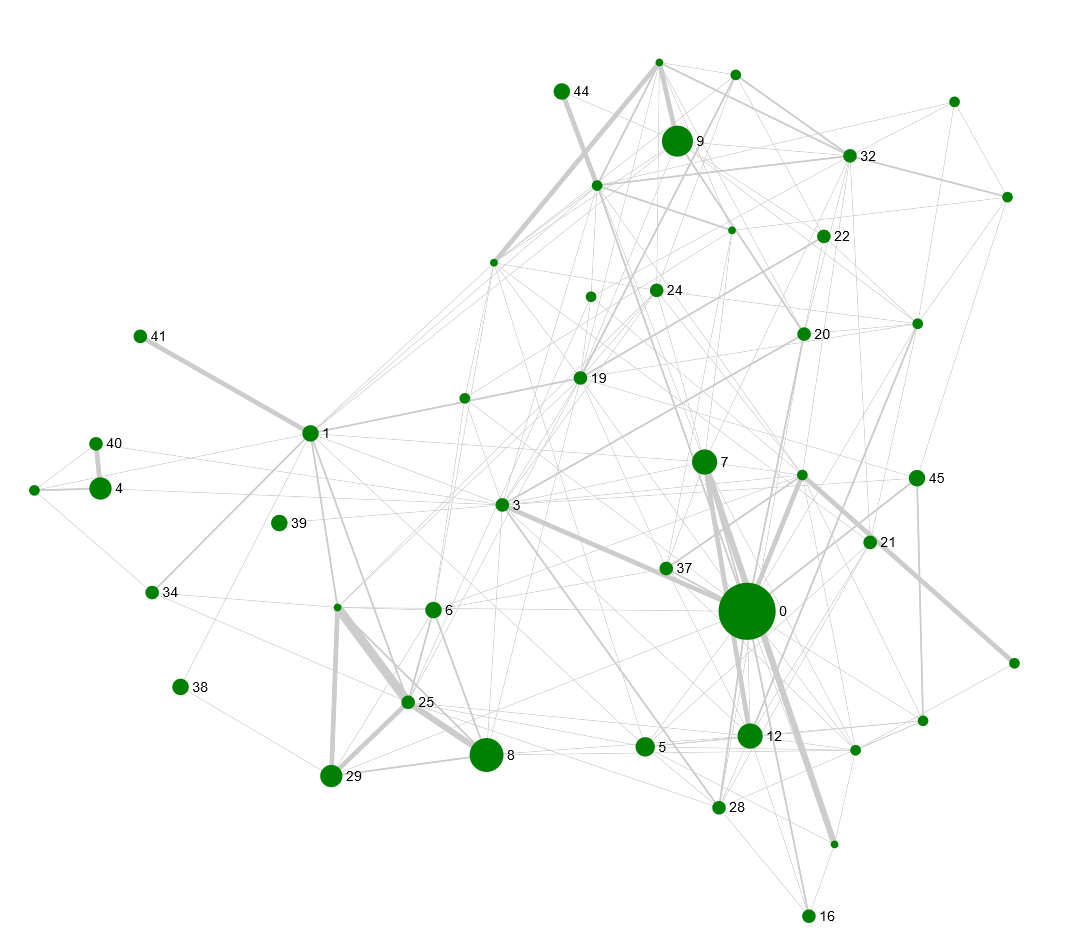
\includegraphics[width=\linewidth]{images/network_plots/rsog_c.png}
        \caption{Topic Network of RSOG Journal}
        \label{fig:rsog_topic_network}
    \end{subfigure}

    \vspace{1em} % Space between rows

    % Second row of images
    
    \begin{subfigure}[b]{0.7\columnwidth}
        \centering
        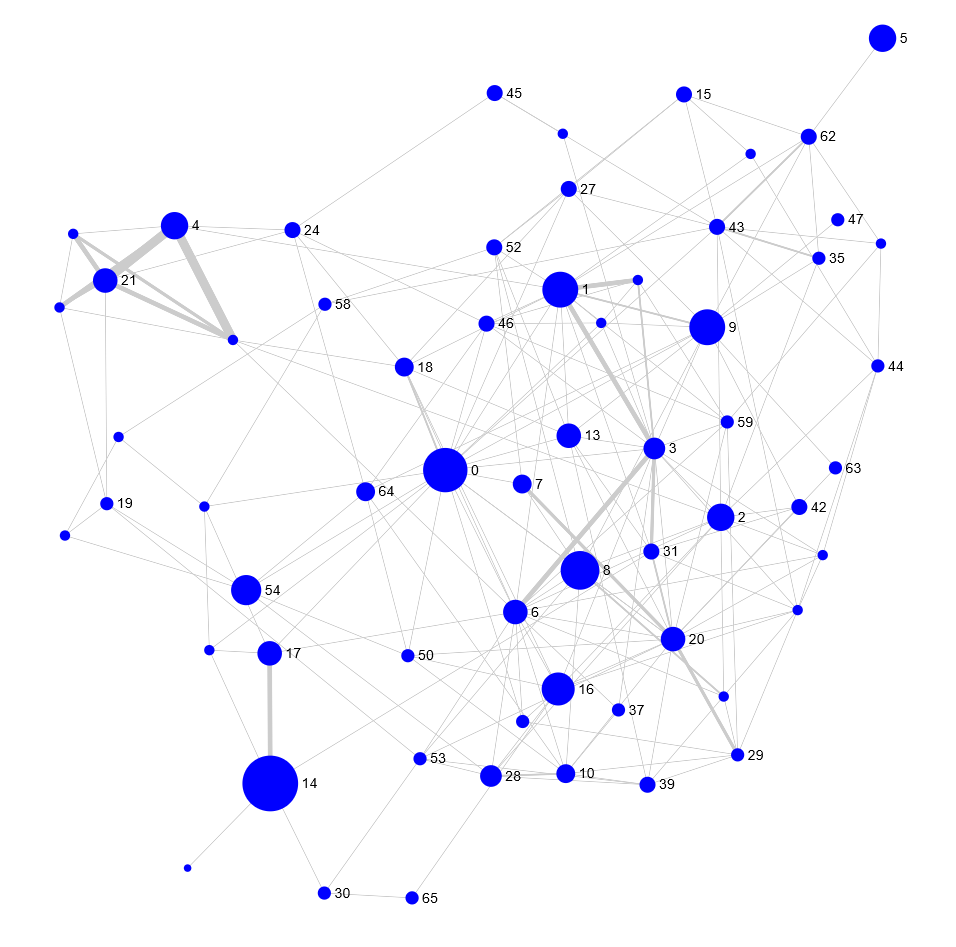
\includegraphics[width=\linewidth]{images/network_plots/ss_c.png}
        \caption{Topic Network of SusSci Journal}
        \label{fig:ss_topic_network}
    \end{subfigure}
    \hfill
    \begin{subfigure}[b]{0.7\columnwidth}
        \centering
        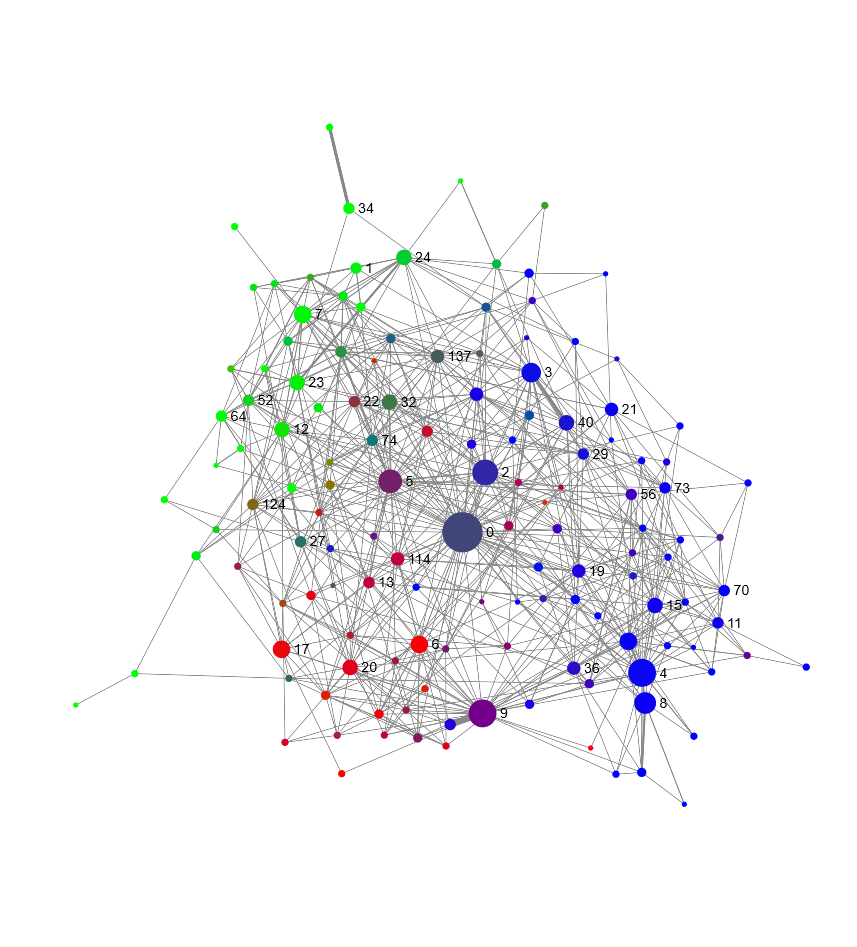
\includegraphics[width=\linewidth]{images/network_plots/3j.png}
        \caption{Topic Network of combined three journals}
        \label{fig:3j_topic_network}
    \end{subfigure}

% Overall caption for the figure
    \caption{Nodes in the topic network represents the dominance of a topic within the journal(s). Edge represents the co-occurrence of a topic in the scientific articles. Color in the (d) represents the shift of authors discourse. Red represent purely EIST discourse, Green represent purely RSOG discourse and Blue represent purely SusSci discourse }
    \label{fig:all-pics}
\end{figure}

\begin{figure}[ht]
    \centering
    %\vspace{1em} % Space between rows

    % Third row of images
    \begin{subfigure}[b]{0.7\columnwidth}
        \centering
        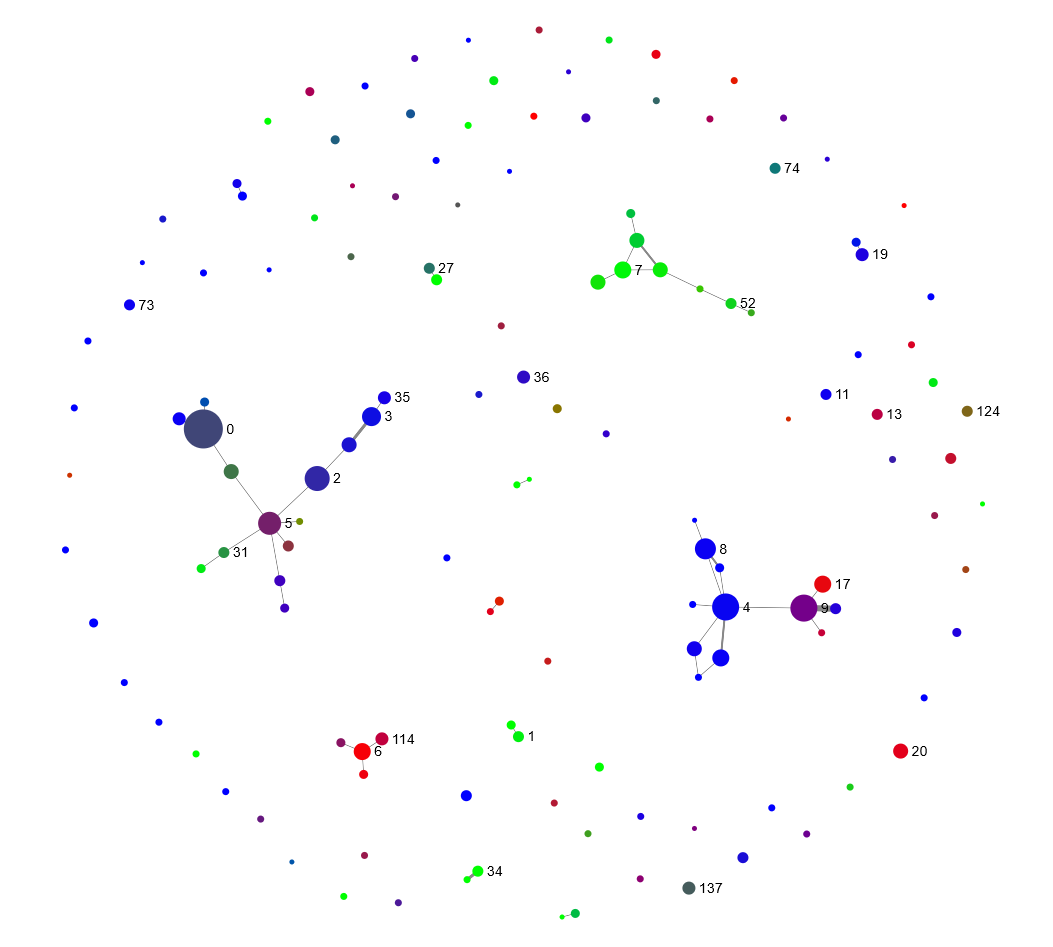
\includegraphics[width=\linewidth]{images/network_plots/3j_3+.png}
        \caption{Topic Network of combined 3 journals with co-occurrence of topic in more than three scientific articles }
        \label{fig:3j_topic_network_w3+}
    \end{subfigure}
    \hfill
    \begin{subfigure}[b]{0.7\columnwidth}
        \centering
        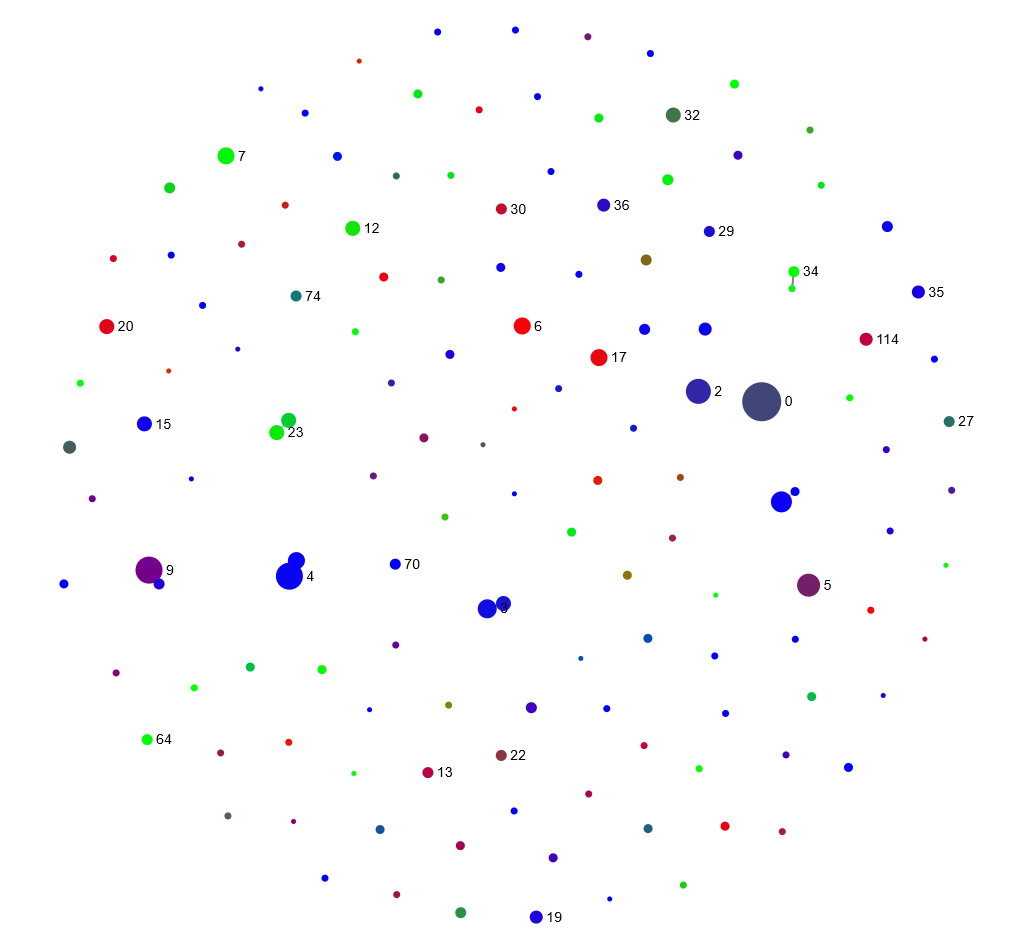
\includegraphics[width=\linewidth]{images/network_plots/3j_5+.png}
        \caption{Topic Network of combined 3 journals with co-occurrence of topic in more than five scientific articles }
        \label{fig:3j_topic_network_w5+}
    \end{subfigure}

    % Overall caption for the figure
    \caption{Node and edge are created in similar fashion as previous network plots. However, in order to show highly co-occurring topics, edges with weight less than 3 in (a) and 5 in (b) are removed.}
    \label{fig:all-pics}
\end{figure}

These metrics offer a quantified understanding of how these interdisciplinary topics are interconnected, their relative importance, and their roles in the larger research landscape. For Visualization, the network topology was visualized using Gephi, a tool renowned for its robustness in handling complex networks. The graphical representation furnished by Gephi and iterated using Nansi, an online tool, enables an intuitive grasp of the complex relationships and structures among the three journal topics, thus shedding light on potential avenues for future interdisciplinary research. By adopting these advanced techniques for topic trajectories and network analysis, our methodology transcends traditional literature review methods. It enables a nuanced understanding of the evolving academic landscape at the intersection of sociology, environmental innovation, and sustainability science, thereby illuminating underlying patterns and emerging trends.
\subsubsection{Identification of Topic Trajectories - Hot, Cold, Wallflower,Evergreen and Revival}
To map the Dynamic Landscape between the three journals  we used a new python code based on Antons 2017, 2018 and their analysis, to compute linear time trends for each of the 138 identified topics. These trends are based on their yearly publication frequencies. This allowed us to categorize topics as either \textbf{"hot"} (exhibiting a positive time trend) or \textbf{"cold"} (exhibiting a negative time trend). 
\begin{figure}[ht]
    \centering
    % Top right image
    \begin{subfigure}[b]{0.7\linewidth}
        \centering
        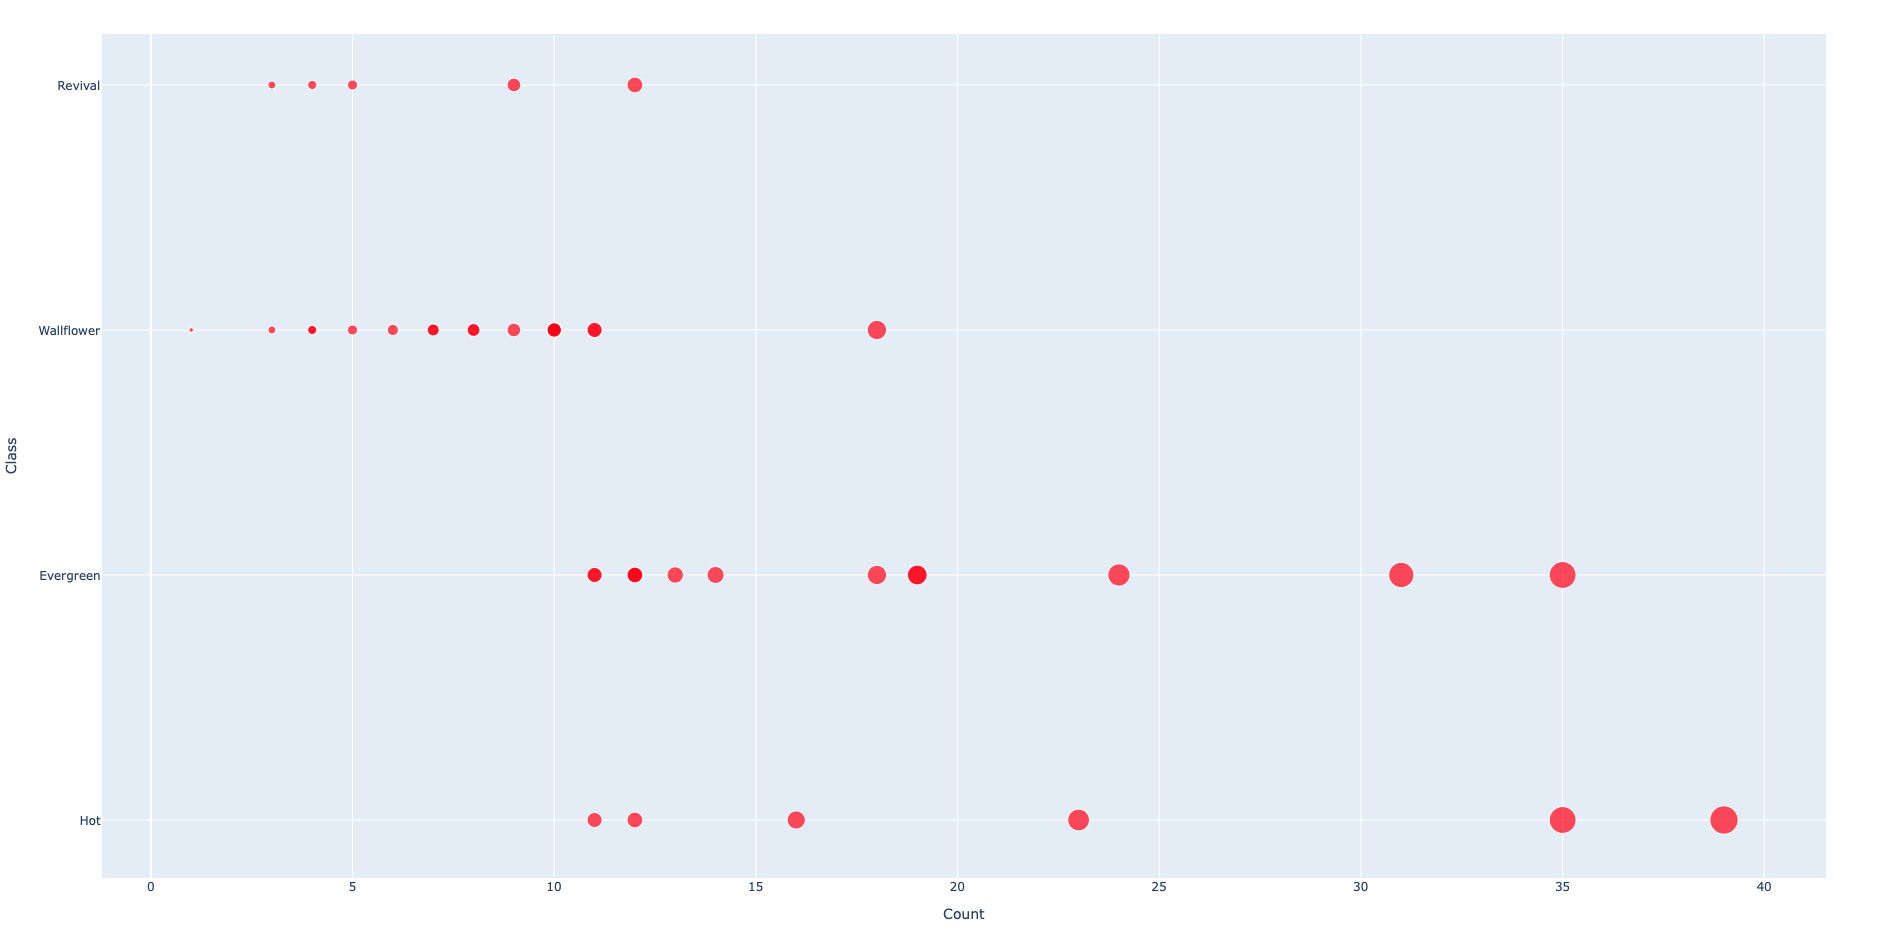
\includegraphics[width=\linewidth]{images/temporal_plots/eist_temporal_pattern.png}
        \caption{Temporal Plot for EIST Topics}
        \label{fig:second-image}
    \end{subfigure}

    \vspace{1em} % Space between the top and bottom rows

    % Bottom left image
    \begin{subfigure}[b]{0.7\linewidth}
        \centering
        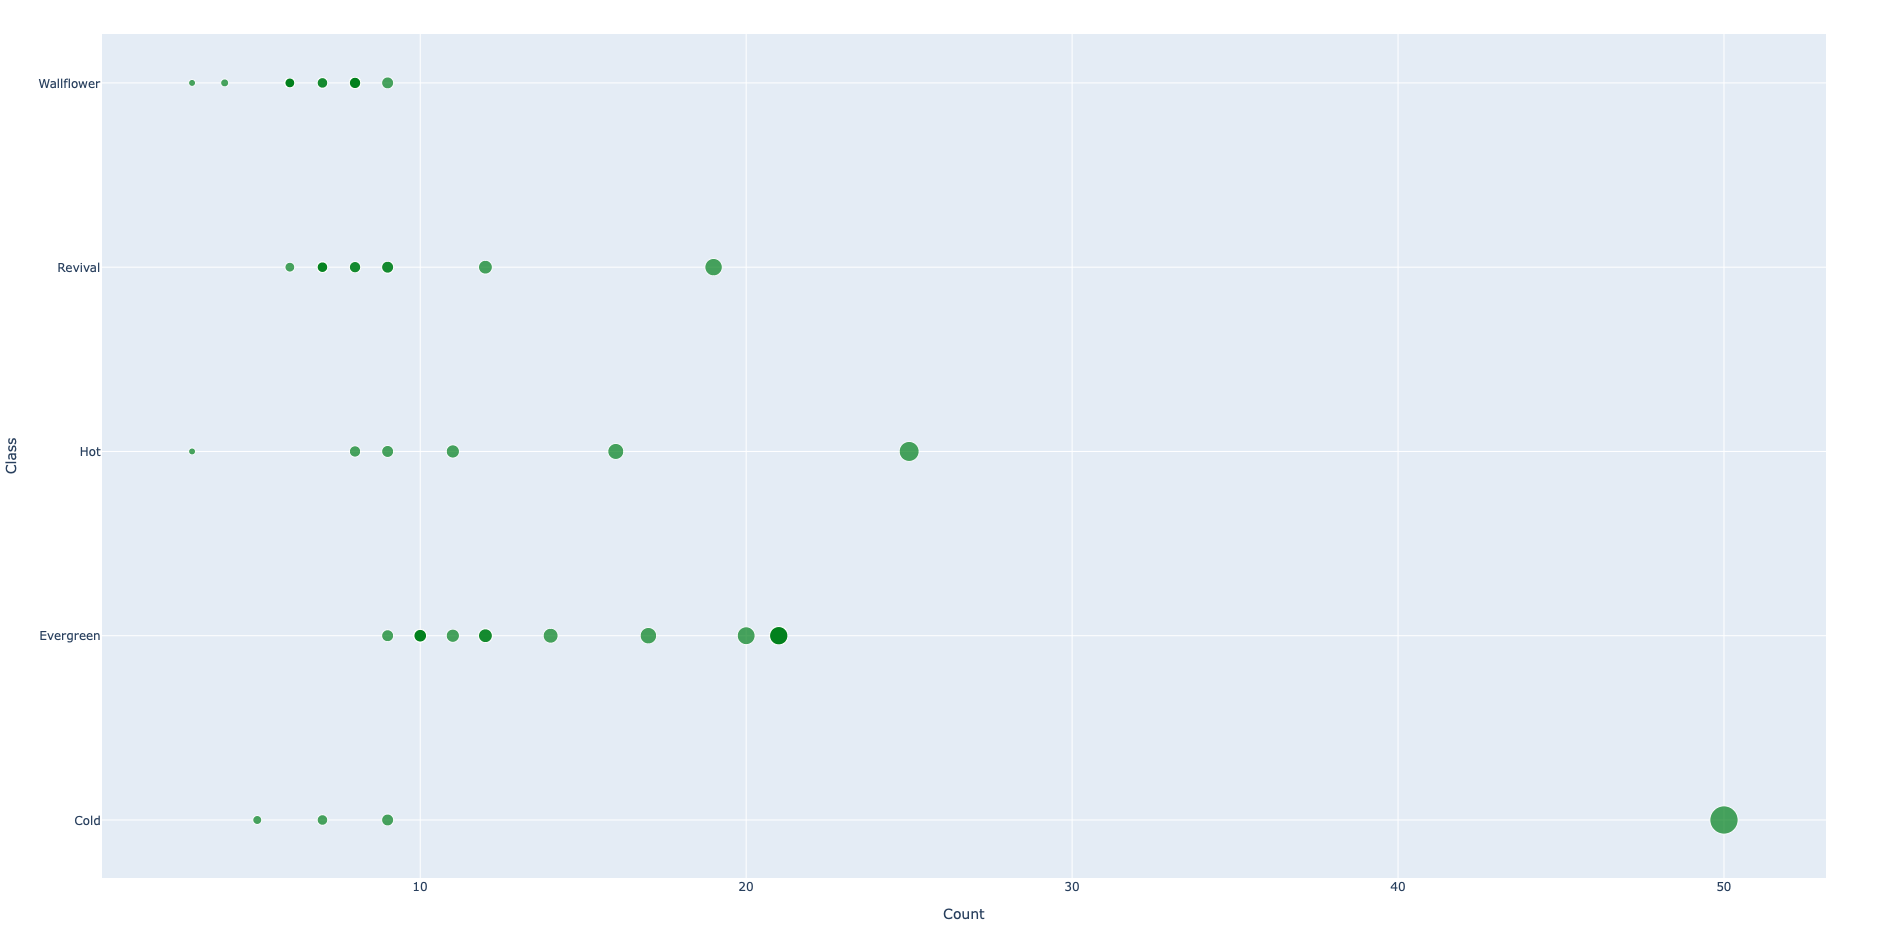
\includegraphics[width=\linewidth]{images/temporal_plots/rsog_temporal_pattern.png}
        \caption{Temporal Plot for RSOG Topics}
        \label{fig:third-image}
    \end{subfigure}
    \hfill % Space between the bottom two images
    % Bottom right image
    \begin{subfigure}[b]{0.7\linewidth}
        \centering
        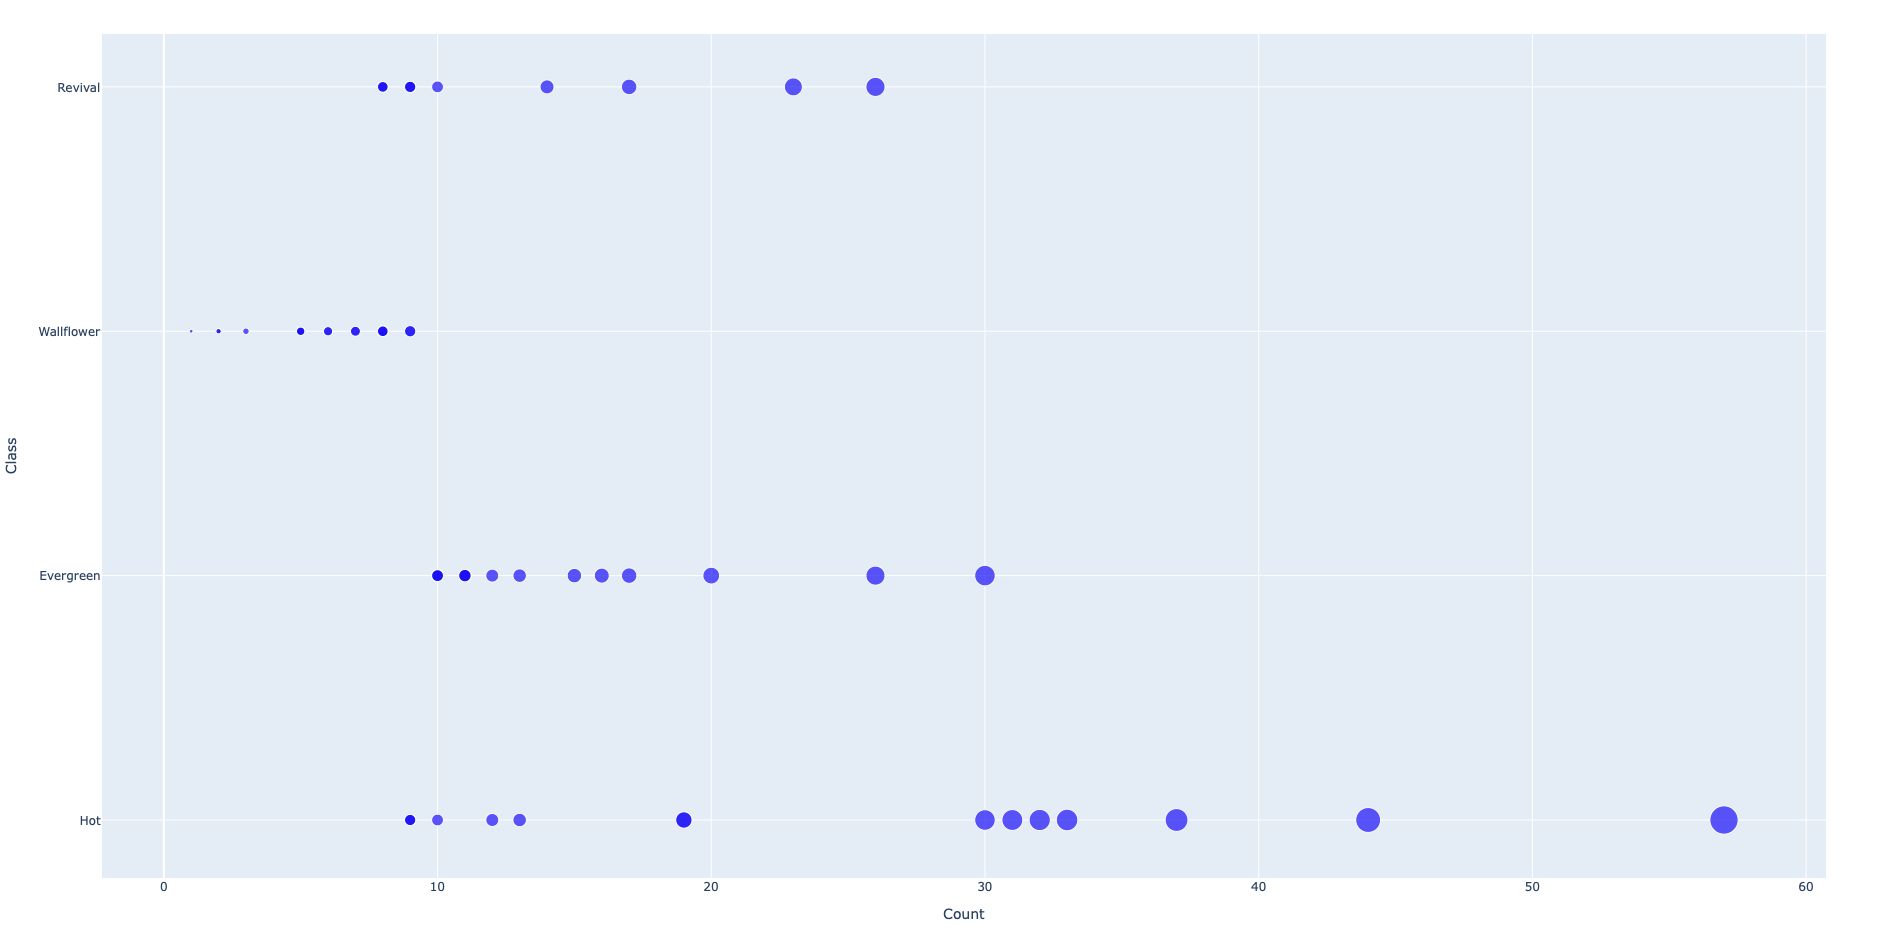
\includegraphics[width=\linewidth]{images/temporal_plots/ss_temporal_pattern.png}
        \caption{Temporal Plot for SUSSCI Topics}
        \label{fig:fourth-image}
    \end{subfigure}

    % Overall caption for the figure
    \caption{Temporal Plots Per Journal (Hot, Cold, Wallflower, Reviving and Evergreen}
    \label{fig:overall}
\end{figure}


\begin{figure}
    \centering
    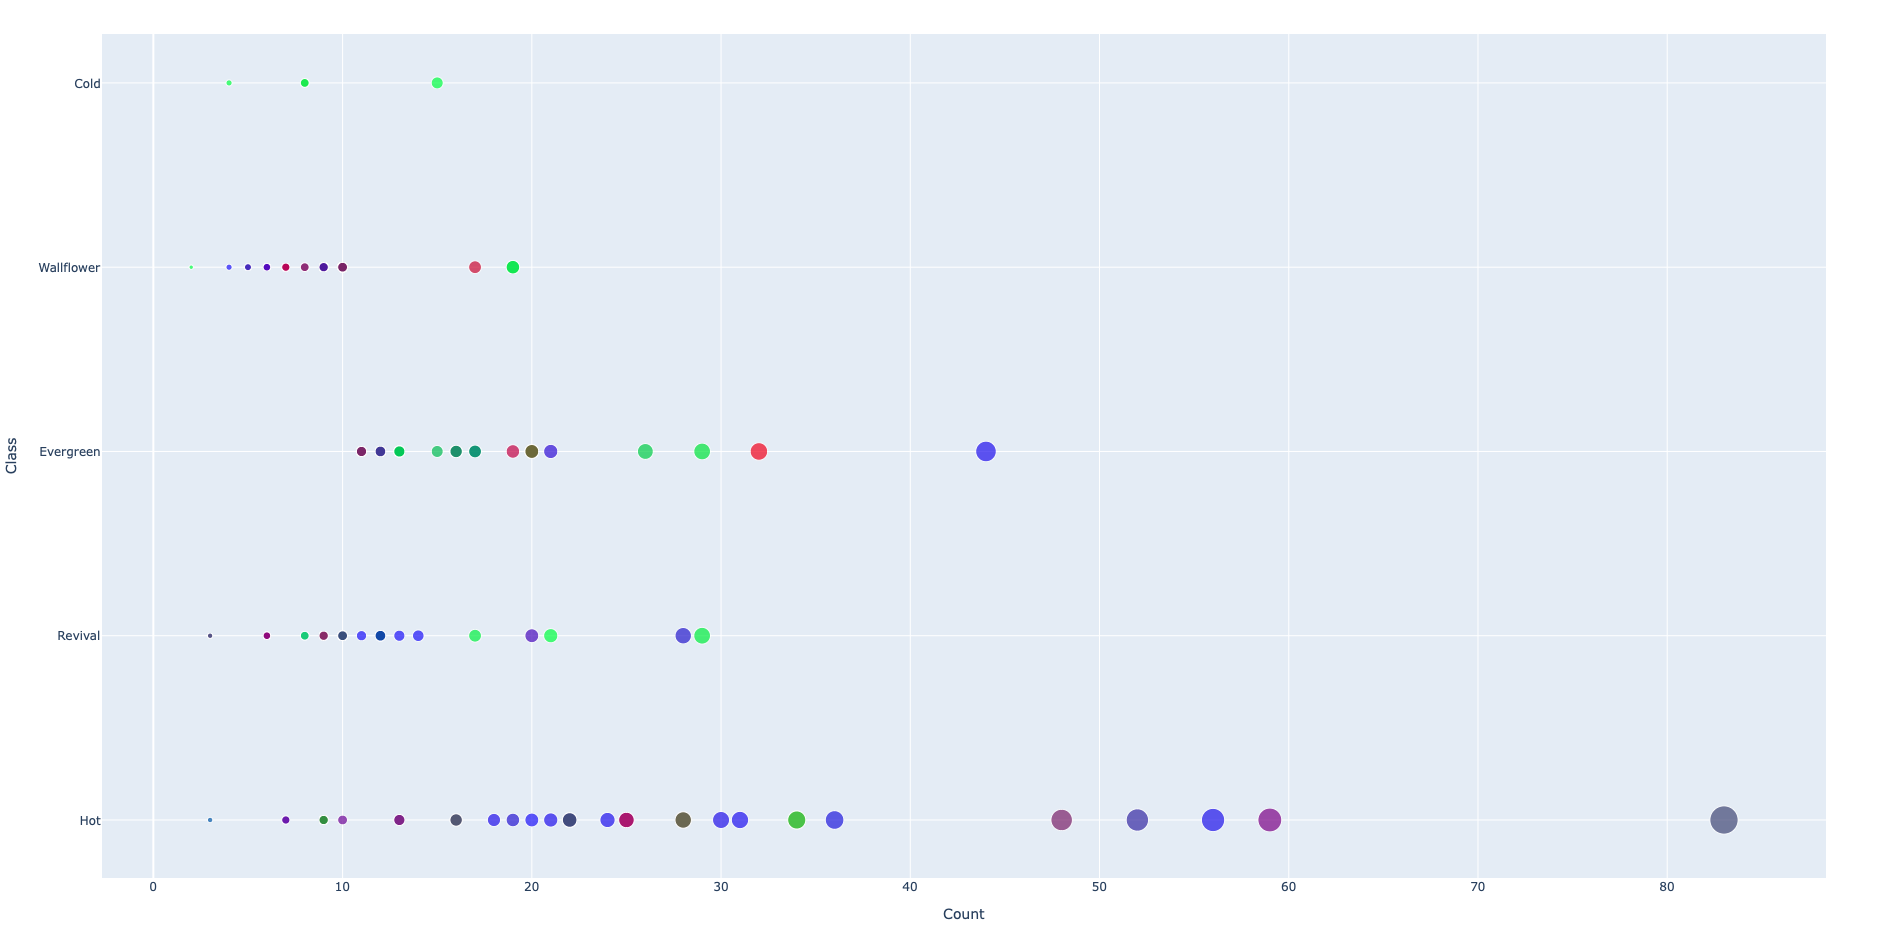
\includegraphics[width=\linewidth, height=0.5\linewidth]{images/temporal_plots/3j_temporal_pattern.png}
    \caption{Topic trajectories of combined three journals. Each point in the plot represents a topic with corresponding trajectory class in Y-axis and number of scientific article it belong to on X-axis. Color represents the proportion of topic in three journals with Red representing 100\% EIST, Green representing 100\% RSOG and Blue representing 100\% SusSci.}
    \label{fig:3j_temporal}
\end{figure}


\subsection{Cross-Disciplinary Patterns}
Here we have explicitly followed the framework of \cite{griffiths_finding_2004} as suggested by Antons and colleagues. This dynamic landscape is instrumental for tracing the evolutionary patterns of topics at the crossroads of sociology, environmental innovation, and sustainability science, and for discerning potential future research trajectories.
\paragraph{Insight 1: Interdisciplinary Research on Sociology, Environmental Innovation, and Sustainability Science}
Our study uncovers 138 unique topics within the intersection of sociology, environmental innovation, and sustainability science. This landscape of research appears to balance between empirical, theoretical, and a few methodological topics.
The labels first assigned to each topic is generic. The topic's overarching classification has been synthesized in the appendix . see \ref{fig:Thematic Correlations Across Journals}.
The number of articles and their distribution vary significantly across the three journals. Table 3 outlines this topic landscape, detailing:
The temporal trajectory of each topic
indicating whether it is 'hot' or 'cold' based on publication trends.
\paragraph{Insight 2: Varying Topic Contributions Across Journals on Sociology, Environmental Innovation, and Sustainability Science}
The extent to which each of the three journals—sociology of organizations, environmental innovation, and sustainability science—contributes to the identified topics shows considerable variation. Notably, sustainability science research has contributed the most of the 138 topics, indicating its broad scope and interdisciplinary nature. On the other hand, articles from RSOG and EIST focus on more specialized subsets of these topics, reflecting the specific orientations of these journals. This also means the temporal trajectories for each journal are varying. This disparity in topic coverage highlights the potential complementary roles these journals play in shaping the academic landscape. It also points to the need for mapping the interstice/potential areas where increased interdisciplinary collaboration could yield valuable insights for each journal.
\paragraph{Insight 3: Methodological Maturity and Focus in Sociology, Environmental Innovation, and Sustainability Science Research} The research in the three domains—sociology of organizations (RSOG), environmental innovation (EIST), and sustainability science (SUSSCI)—demonstrates distinct levels of methodological maturity and focus. Specifically, articles from SUSSCI are generally more methodologically mature, often employing qualitative and quantitative methods and focusing on issues of broad academic relevance.While RSOG has been mostly qualitative and theoretical,with EIST being mostly qualitative. This likely reflects the journal's foundations in case study based research. SUSSCI shows its interdisciplinary nature which draws from well-established quantitative disciplines like economics and systems science.

% Place the first image centered on its own page
\begin{figure}[p]
    \centering
    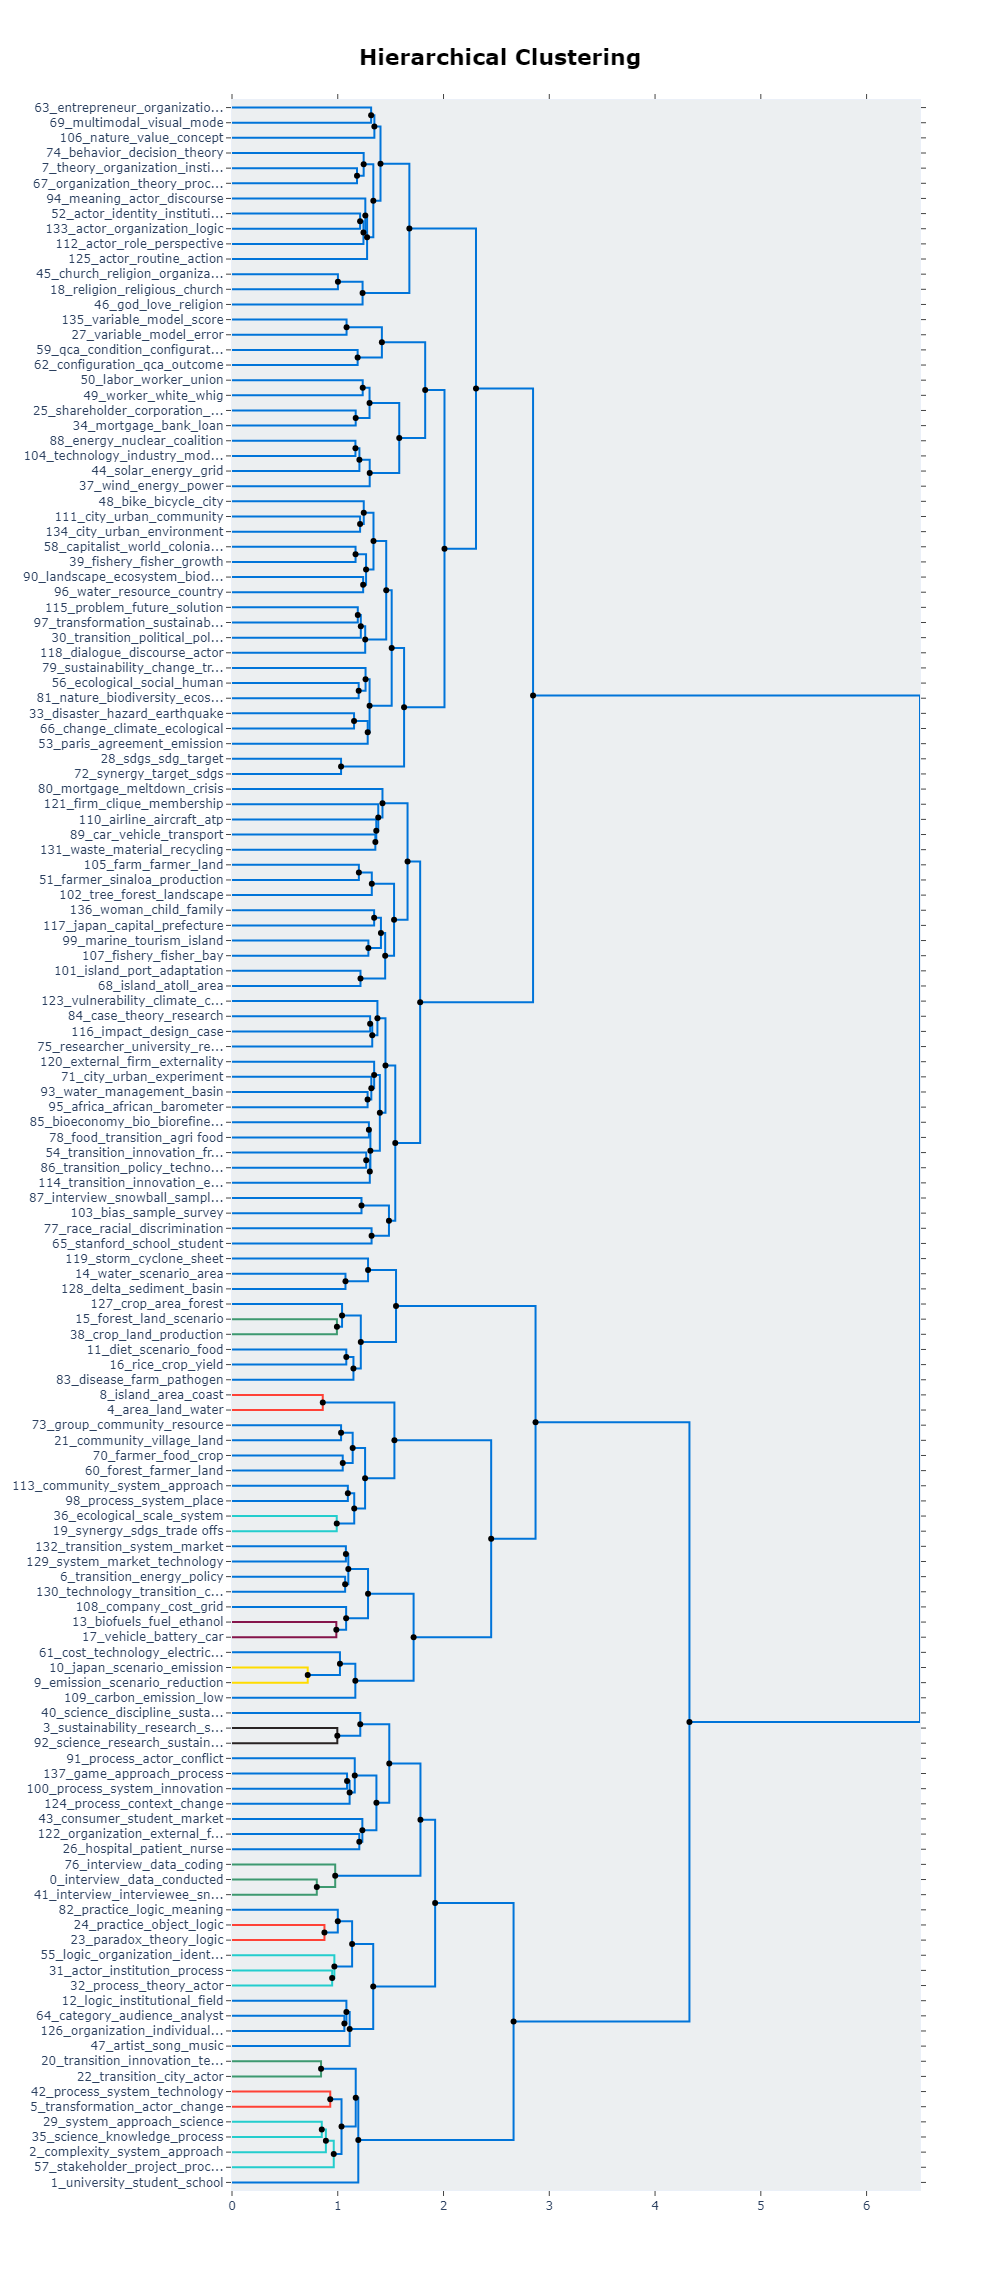
\includegraphics[width=0.5\textwidth]{images/3j_hplot.png}
    \caption{Three Journal Hierarchical Topic Plot}
    \label{fig:3j-hplot}
\end{figure}

% Place the other three images on a separate full page
\begin{figure}[p]
    \centering
    % Top image
    \begin{subfigure}[b]{0.5\textwidth}
        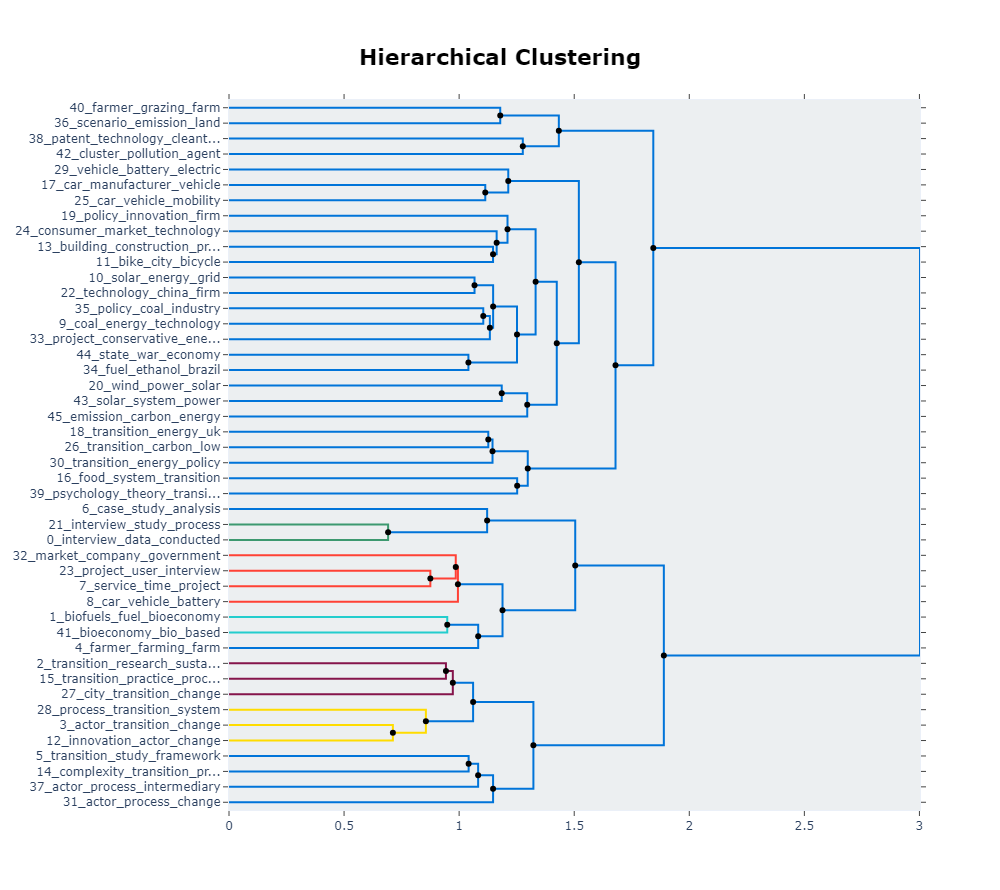
\includegraphics[width=\linewidth]{images/eist_hplot.png}
        \caption{Hierarchical Topic Plot for EIST}
        \label{fig:eist-hplot}
    \end{subfigure}
        \vspace{1em} % Space between the images
        % Bottom left image
    \begin{subfigure}[b]{0.3\textwidth}
        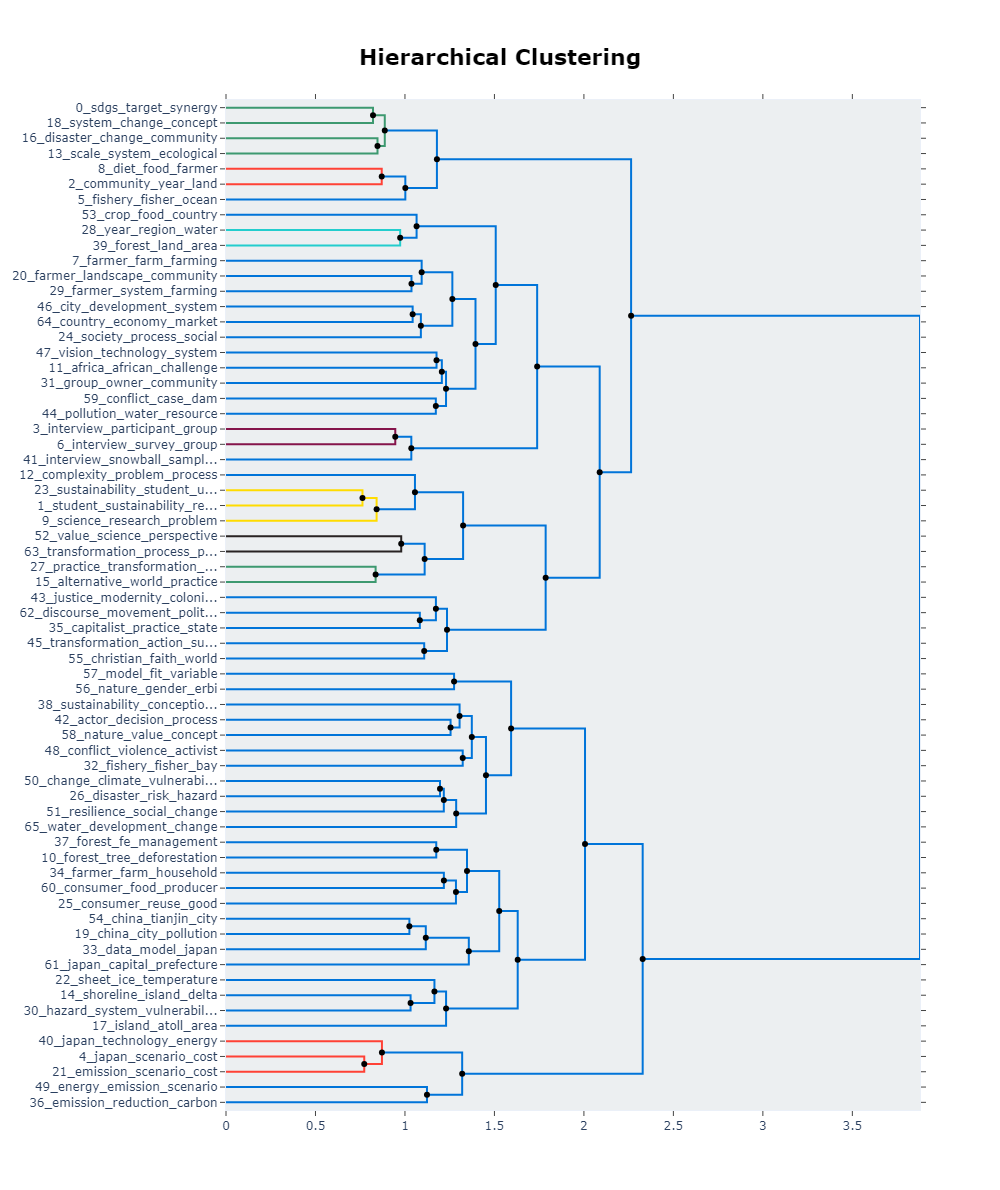
\includegraphics[width=\linewidth]{images/sussci_hplot.png}
        \caption{Hierarchical Topic Plot for SUSSCI}
        \label{fig:sussci-hplot}
    \end{subfigure}
    \hfill % Space between the two bottom images
    % Bottom right image
    \begin{subfigure}[b]{0.5\textwidth}
        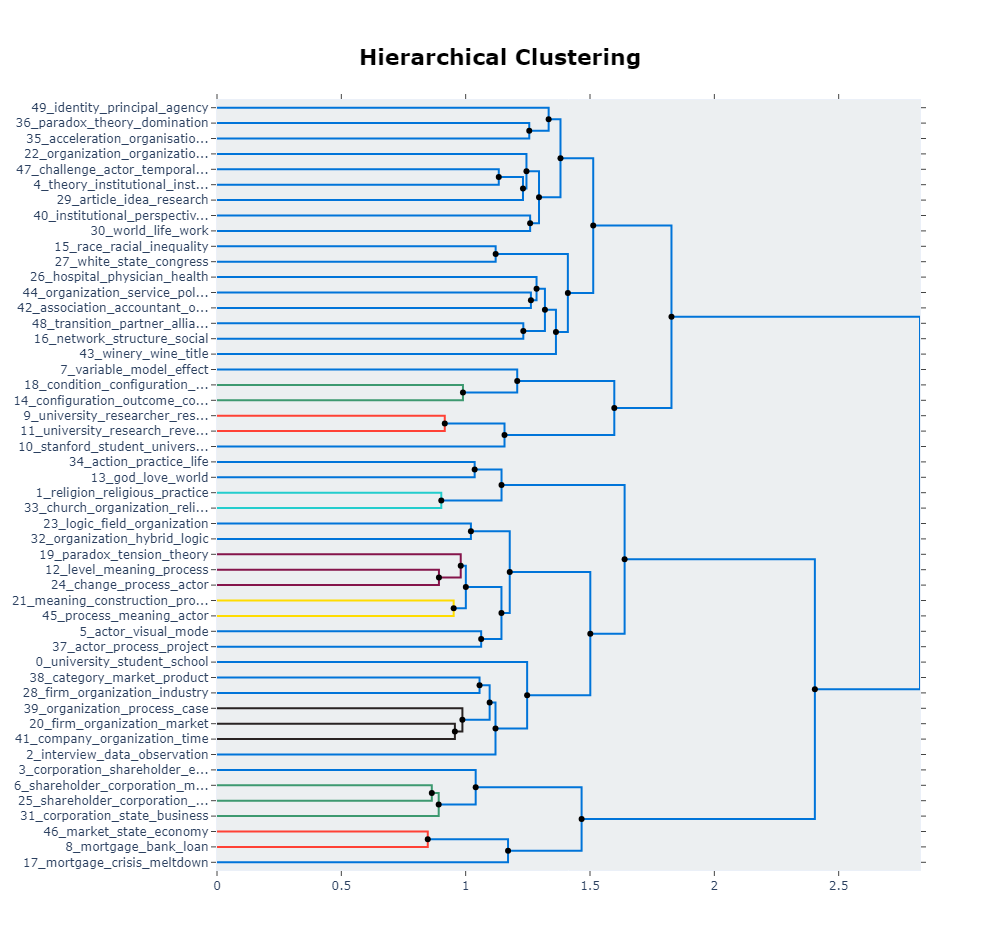
\includegraphics[width=\linewidth]{images/rsog_hplot.png}
        \caption{Hierarchical Topic Plot for RSOG}
        \label{fig:rsog-hplot}
    \end{subfigure}
    \caption{Hierarchical Topic Plots for Individual Journals}
    \label{fig:individual-hplots}
\end{figure}

In contrast, research from EIST and RSOG tends to rely more on qualitative and conceptual methodologies.While EIST and SUSSCI have system level topics.RSOG often address topics of immediate organizational or field level relevance, indicating a potential for complementary work as sustainability transitions has been calling for more sociology of actors\cite{upham_actors_2021,upham_rethinking_2020,wittmayer_actor_2017,avelino_multi-actor_2017,de_haan_towards_2010,bogel_role_2018} and more applied focus on agency aspects of transition governance\cite{frantzeskaki_governing_2012,loorbach_transition_2013}. The differences in methodological approaches across these journals not only show their unique contributions but also suggest opportunities for methodological cross-pollination and for addressing a broader set of questions in future research.
Of all three only RSOG has used multimodal data and analysis techniques. All three have used network analysis, and analyzed verbal text. Visual text is yet to be adopted as a data source in EIST and SUSCI.
\paragraph{Insight 4: Topic Connectivity in Sociology of Organizations, Environmental Innovation, and Sustainability Science Research}
\begin{figure}
    \centering
    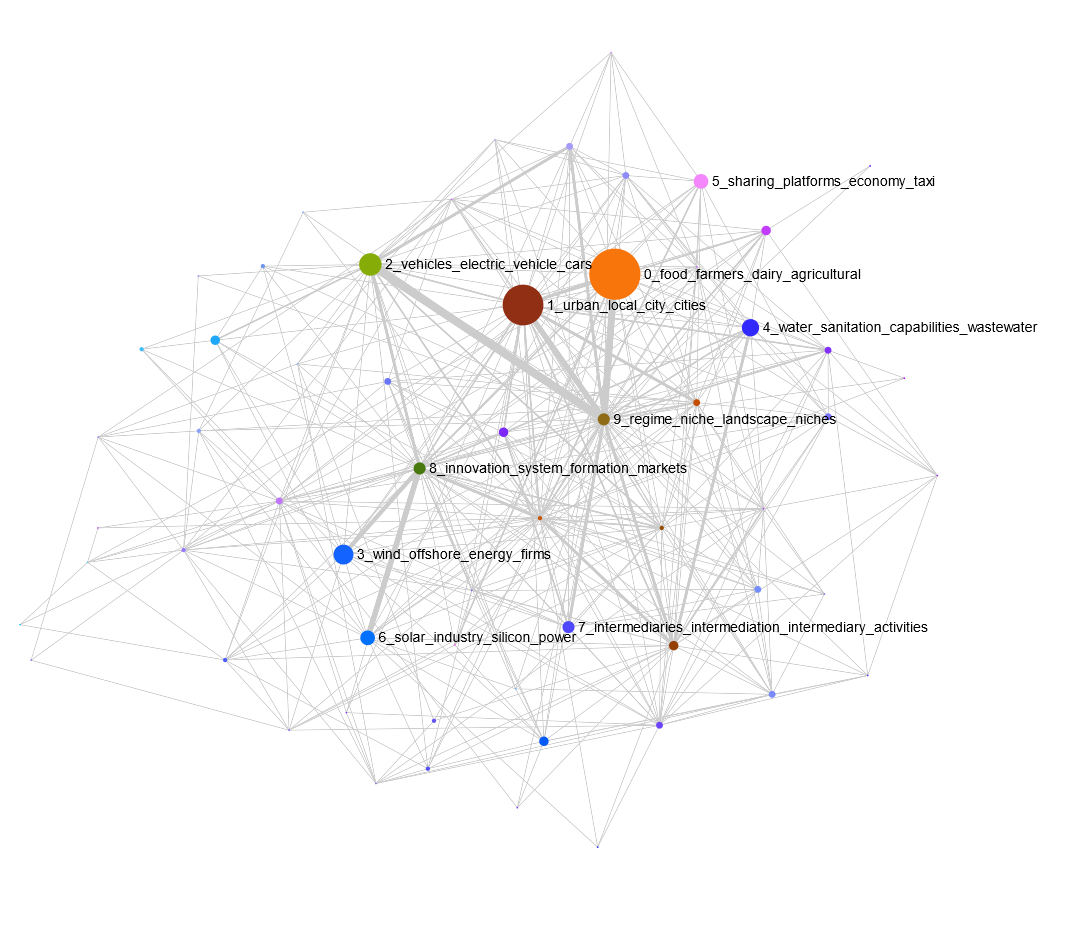
\includegraphics[width=0.7\linewidth]{images/eist_topic_network.png}
    \caption{EIST Topic Networks}
    \label{fig:enter-label}
\end{figure}
\begin{figure}
    \centering
    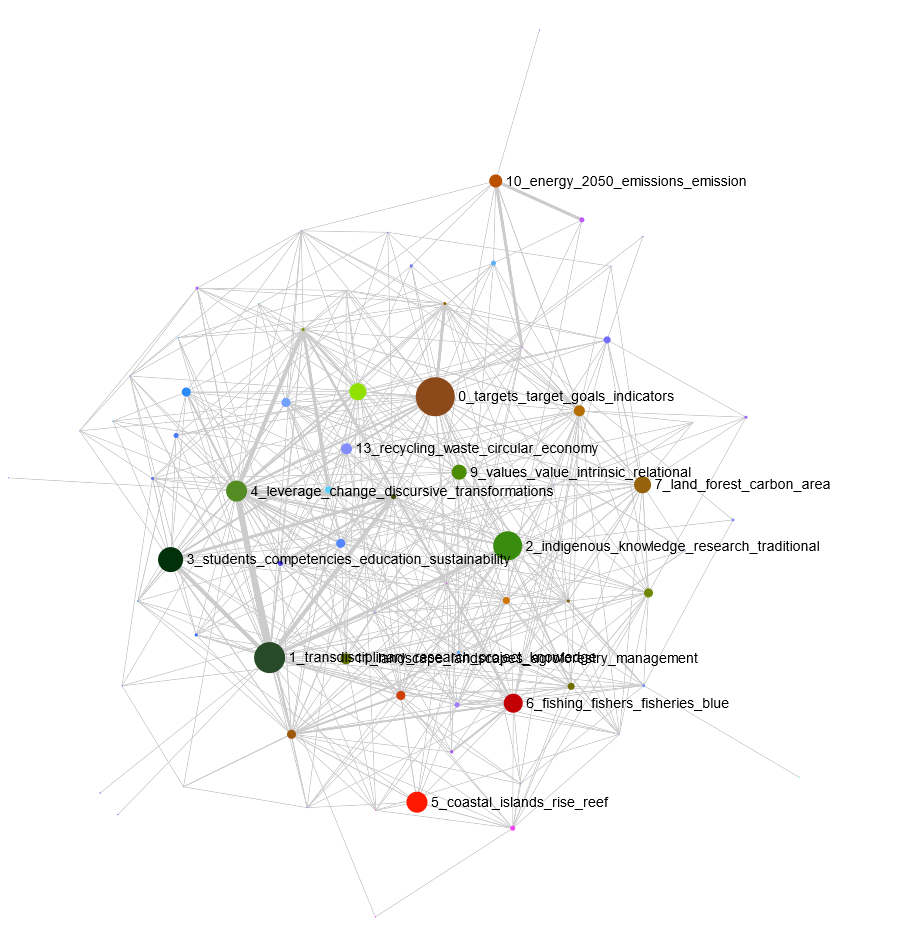
\includegraphics[width=0.7\linewidth]{images/ss_topic_network.png}
    \caption{SUSSCI Topic Networks}
    \label{fig:enter-label}
\end{figure}
\begin{figure}
    \centering
    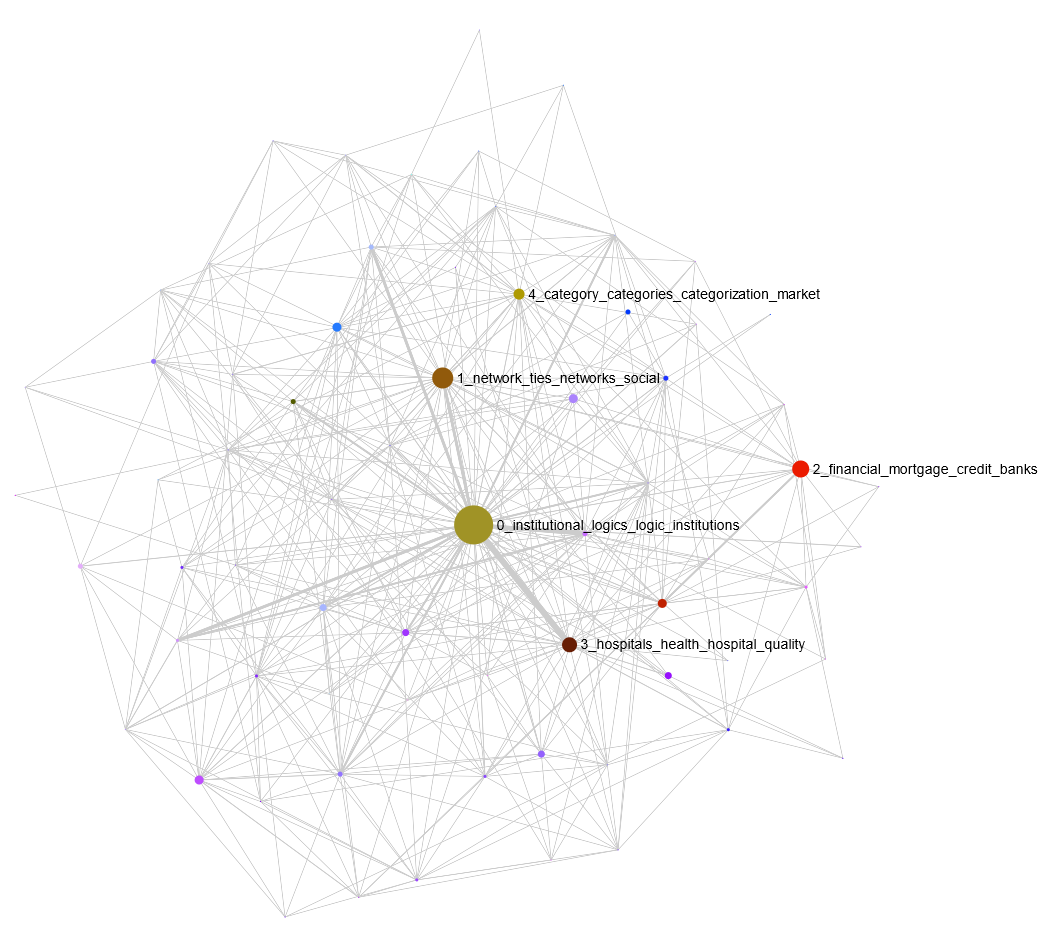
\includegraphics[width=0.7\linewidth]{images/rsog_topic_network.png}
    \caption{RSOG Topic Networks}
    \label{fig:enter-label}
\end{figure}
The network analysis of topics within the three selected journals—RSOG, EIST, and SUSSCI—reveals a loosely connected topic landscape. This suggests that the domains of sociology of organizations, environmental innovation, and sustainability science are far from being integrated or consolidated as singular or interrelated fields of study.This is not necessarily a negative occurrence.What could be beneficial is more interstitial research\cite{Korff2015} 
Such loose connectivity could indicate multiple phenomena: research silos within each domain, a lack of interdisciplinary work bridging these journals, or perhaps the nascent stages of emerging sub-disciplines. This finding aligns with the broader literature, which often treats these domains as distinct fields of inquiry. The loosely connected network of topics provides both a challenge and an opportunity. The challenge lies in the potential for fragmentation and redundancy; the opportunity lies in the room for future research to bridge these gaps, fostering a more integrated and comprehensive understanding of the interstitial space between sociology of organizations, environmental innovation, and sustainability science.
\subsection{Methodological Validation}

The mapping of topics and interstitial authors provides a foundation for future synthesis of a metaheory for socio-institutional analysis particularly one drawing on sociology\cite{Loorbach2017}. The interstice of Research in the Sociology of Organizations (RSOG), Environmental Innovation and Societal Transitions (EIST), and Sustainability Science (SUSSCI) is an academic frontier teeming with untapped potential. While each journal covers a distinct domain, their intersection holds the promise of transformative insights into socio-institutional dynamics that govern sustainability transitions. However, the absence of a structured pathway for cross-disciplinary engagement has left this interdisciplinary space largely uncharted. Building on our computational literature review and network analysis, we present an empirically grounded research agenda designed to catalyze interdisciplinary research at this intersection. In light of the findings and insights derived from the actor landscape and topic modeling, it's evident that there is a compelling need for a more integrated approach to research at the intersection of Research in the Sociology of Organizations (RSOG), Environmental Innovation and Societal Transitions (EIST), and Sustainability Science (SUSSCI). This section proposes an agenda aimed at fostering this integration through socio-institutional analysis.
\subsection{Proposing Five Research Directions and 15-Point Action Plan}
\label{sec:fiverd_15point}
\begin{enumerate}
    \item Research Direction 1: Link Disconnected Topics within the Research Network
\begin{itemize}
    \item Mechanism 1.1: Apply theoretical perspectives to explore socio-institutional phenomena not previously studied in STR
    \item Mechanism 1.2: Link different Socio-institutional phenomena that could stimulate new knowledge on transition dynamics in STR.
    \item Mechanism 1.3: Foster the inclusion of peripheral topics into the core research network
    \item Mechanism 1.4 : Revive Cold Topics via special issues and joint conferences.
    \end{itemize}
    \item Research Direction 2: Increase the Generalizability of RSOG,EIST and SUSSCI.
\begin{itemize}
    \item Mechanism 2.1: Replicate existing studies in new contexts.
    \item Mechanism 2.2: Investigate topics not previously covered.
    \item Mechanism 2.3: Investigate sparsely connected topics in new contexts.
    \end{itemize}
    \item Research Direction 3: Expand Theoretical Scope via Interdisciplinary Theory Building
\begin{itemize}
    \item Mechanism 3.1: Encourage theoretical expansion.
    \item Mechanism 3.2: Build upon peripheral theories to inform discourse.
    \item Mechanism 3.3: Comparative Analyses of Same Phenomena using multiple theories.
    \end{itemize}
    \item Research Direction 4: Advance Methodological Innovation and Interaction Between the Three Spheres.
\begin{itemize}
    \item Mechanism 4.1: Adopt underutilized methods and data (e.g multimodal analysis/data).
    \item Mechanism 4.2: Use qualitative methods for topics dominated by quantitative research and vice versa.
    \end{itemize}
    \item Research Direction 5: Data Driven Theory Guided Socio-Institutional Analysis via Annotation and Knowledge Sharing.
\begin{itemize}
    \item Mechanism 5.1: Shared Database,Tasks like in Computational Social Science .
    \item Mechanism 5.2: Meta-Analysis and Systematic Reviews to Develop a Full Metatheory for SIA,\cite{edwards 2014,de haan et al 2021}.
    \item Mechanism 5.3: Open Science Annotation to boost Socio-Institutinal Analysis at scale.
\end{itemize}
\end{enumerate}
By pursuing this agenda, the academic community can move toward a more integrated and impactful body of research that fully exploits the synergies between sociology, environmental innovation, and sustainability science. This would represent a significant advancement in our ability to address the complex, interrelated challenges that characterize the contemporary socio-environmental landscape.

\section{Methodological Contributions}
\subsection{Advancements in Computational Literature Review - Beyond LDA}
Leveraging LLMs for topic labelling, using BERTopic for validating and exploring different topic combinations especially when it becomes too computationally expensive to run lda on servers as text corpus increases.
\subsection{Innovative Integration of Social-X Ray Methodology in STR}
We looked at semantic dimensions as well as social dimensions which can be more central in future CLR proceedures.
\onecolumn 
%\begin{landscape}
\begin{longtable}{|p{0.3\textwidth}|p{0.7\textwidth}|}
\caption{Overview of Research Priorities and Guidelines.}
\label{tab:my-table_rpg_3j}\\
\hline
\textbf{Research Direction and Mechanism} & \textbf{Exemplary Research Questions and Journals} \\
\hline
\endfirsthead

\multicolumn{2}{c}%
{{\bfseries Continued from previous page}} \\
\hline
\textbf{Research Direction and Mechanism} & \textbf{Exemplary Research Questions and Journals} \\
\hline
\endhead

\hline \multicolumn{2}{r}{{Continued on next page}} \\ \hline
\endfoot

\hline \hline
\endlastfoot
% Research Direction 1
\textbf{Research Direction 1: Link Disconnected Topics within the Three Journal Network} & \\
Mechanism 1.1: Apply Theoretical Perspectives (RSOG) & 
- How can organizational theories on fields enhance understanding of multi-actor constellations in environmental innovation and societal transitions? \\
& - What role do organizational structures play in shaping sustainability practices? \\
Mechanism 1.2: Link Different Phenomena (EIST) & 
- How do technological innovations in sustainability impact organizational dynamics? \\
& - What are the societal implications of transitioning to green technologies? \\
Mechanism 1.3: Foster Inclusion of Peripheral Topics (SUSSCI) & 
- How does community engagement in sustainability projects impact long-term outcomes? \\
& - What is the role of grassroots movements in shaping sustainability policies? \\
Mechanism 1.4: Revive Cold Topics (RSOG, EIST, SUSSCI) & 
- What past sustainability theories or models need revisiting in the current environmental context? \\
& - How can interdisciplinary conferences rejuvenate interest in overlooked sustainability issues? \\
\hline
% Research Direction 2
\textbf{Research Direction 2: Increase the Generalizability of Research} & \\
Mechanism 2.1: Replicate Studies in New Contexts (EIST) & 
- Are models of environmental innovation applicable across different socio-economic contexts? \\
Mechanism 2.2: Investigate Uncovered Topics (SUSSCI) & 
- What are the emerging challenges in urban sustainability in developing countries? \\
Mechanism 2.3: Investigate Sparsely Connected Topics (RSOG) & 
- How do organizational changes in response to societal transitions compare across cultures? \\
\hline
% Research Direction 3
\textbf{Research Direction 3: Expand Theoretical Scope via Interdisciplinary Theory Building} & \\
Mechanism 3.1: Encourage Theoretical Expansion (RSOG) & 
- How can concepts from environmental sociology reshape organizational strategies? \\
Mechanism 3.2: Build Upon Peripheral Theories (EIST) & 
- What can theories of social change offer to the study of environmental transitions? \\
Mechanism 3.3: Comparative Analyses (SUSSCI) & 
- How do different theoretical frameworks interpret the success of community-led sustainability initiatives? \\
\hline
% Research Direction 4
\textbf{Research Direction 4: Advance Methodological Innovation} & \\
Mechanism 4.1: Adopt Underutilized Methods (EIST) & 
- Can participatory action research reveal new insights into environmental policy development? \\
Mechanism 4.2: Qualitative for Quantitative-Dominated Topics (RSOG) & 
- What qualitative insights can be gained from traditionally quantitative organizational studies? \\
\hline
% Research Direction 5
\textbf{Research Direction 5: Data Driven Theory Guided Socio-Institutional Analysis via Annotation and Knowledge Sharing} & \\
Mechanism 5.1: Open Science Annotation Initiatives (SUSSCI) & 
- How can open data initiatives in sustainability science foster global collaboration between researchers for socio-institutional analysis? \\
Mechanism 5.2: Meta-Analysis and Systematic Reviews (RSOG, EIST, SUSSCI) & 
- What overarching trends can be identified from a meta-analysis of organizational studies on sustainability? \\
Mechanism 5.3: Open Science Annotation to boost Socio-Institutional Analysis at scale.& 
- How can annotations at scale in sustainability science foster global collaboration between researchers for socio-institutional analysis? \\
\end{longtable}
%\end{landscape}
\section{Discussion \& Applications}

\subsection{Limitations of our study and directions for future research.}
\label{sec:limitations}
One of the main limitations of this paper is that it is based on a limited data source. The research was based on a dataset of articles published in the journals EIST, RSOG, and SUSSCI from 2010 to 2022. While these journals are widely recognized as leading outlets for research on the intersection of sociology, environmental innovation, and sustainability science, they are not the only relevant sources of research in these frames. Therefore, the findings and conclusions of this paper may not be generalizable to the broader research landscape in these frames. Another limitation of this paper is that it only focuses on the intersection of sociology, environmental innovation, and sustainability science. While these journals are closely related and share many common themes and concepts, they are not the only disciplines that are relevant to the study of socio-institutional analysis. Other frames, such as economics, psychology, and political science, also have important contributions to make to this area of research. Therefore, the findings and conclusions of this paper may not be fully comprehensive or representative of the broader frame of socio-institutional analysis.
Finally, this paper only uses a single method, computational literature mapping, to analyze the research landscape on the intersection of sociology, environmental innovation, and sustainability science. While this method provides a detailed and quantitative overview of the research landscape, it has its own limitations and assumptions. For example, the topic modeling algorithms used in this paper are based on statistical assumptions and may not capture all of the nuances and complexities of the research landscape. Therefore, the findings and conclusions of this paper should be interpreted with caution and should be complemented by other methods and approaches.


\begin{sidewaystable}
\centering
\caption{Examples of Early CLRs and the Positioning of This Study}
\label{tab:my-table_antonsleague}
\begin{longtable}{|p{3cm}|p{3cm}|p{3cm}|p{3cm}|p{3cm}|p{4cm}|}
\hline
\textbf{Goal} & \textbf{Study} & \textbf{Secondary Goal} & \textbf{Corpus} & \textbf{Techniques} & \textbf{Findings} \\ \hline
\endfirsthead

\multicolumn{6}{c}{{\bfseries Table \thetable\ continued from previous page}} \\ \hline
\textbf{Goal} & \textbf{Study} & \textbf{Secondary Goal} & \textbf{Corpus} & \textbf{Techniques} & \textbf{Findings} \\ \hline
\endhead

\hline \multicolumn{6}{r}{{Continued on next page}} \\ \hline
\endfoot

\hline
\endlastfoot

\textbf{Explicating} & Writer (2019) & Relating & 53k lithium-ion articles & LDA & AI-augmented summarization. \\ \hline
 & Lee and Kang (2018) & Debating & 11.7k tech articles & LDA & Top topics, editor impact. \\ \hline
 & Randhawa et al. (2016) & Envisioning & 321 OI articles & Leximancer, analysis & Identified gaps in OI research. \\ \hline
 & Adeva et al. (2014) & -- & 1.9k medical articles & ATC & Applied ATC in medical reviews. \\ \hline
 & Griffiths and Steyvers (2004) & Envisioning & 28.2k PNAS abstracts & LDA & Trends in PNAS research papers. \\ \hline
\textbf{Envisioning} & Antons et al. (2019) & Debating & 1.6k SMJ articles & LDA, LIWC & Citation impact of topics. \\ \hline
\textbf{Relating} & Chen et al. (2019) & Explicating & IRC literature & Co-citation analysis & Phases of IRC research identified. \\ \hline
 & Antons and Breidbach (2018) & Envisioning & 641 service articles & LDA & Overlap in service innovation and design. \\ \hline
 & Wilden et al. (2018) & Envisioning & 3.9k March articles & Leximancer, coupling & Identified future research directions. \\ \hline
 & Asgari \& Bastani (2017) & -- & Absorptive capacity texts & HDP & Tracked evolution of absorptive capacity. \\ \hline
 & Wilden et al. (2017) & Envisioning & 347 SDL articles & Leximancer, analysis & Evolution of SDL research themes. \\ \hline
\textbf{Debating} & Tuan et al. (2019) & -- & 534 CSRC papers & LIWC & Popularity of CSRC theories analyzed. \\ \hline
 & Hopp et al. (2018) & Explicating & 1.1k innovation articles & LDA & Identified innovation research trends. \\ \hline
 & Tanskanen et al. (2017) & Envisioning & 601 ERM articles & Content analysis & Key themes in ERM research. \\ \hline
\textbf{Envisioning} & \textbf{This Study} & Relating & 2.4k articles & LDA, BERTopic, LLMs & Topic networks and interstitial map of authors identified. \\ \hline

\end{longtable}
\end{sidewaystable}


\subsection{Summary of Key Findings}
It is appararent that our approach is a quantitative synthesis and we therefore encourage others interested to build on our foundational steps towards a metatheory. By making our topic networks and codebase available we invite others to use the themes and topics identified in our work for iteratively designing a more qualitative meta-synthesis of theories for SIA.There is also a need for more research on the intersection of sociology, environmental innovation, and sustainability science, because we used only one sociological journal our discovery is partial, other journals such as organizational theory, organizational studies can be used to replicate our studies, one just has to plug and play the full text of another journal in the triad in order to find more interstial authors and topics. Drawing on the insights from our mapping of topics and authors we encourage future research should focus practical steps to bridging the interstices and  gaps as we only showed how the territory looks. There is a need for more cross-disciplinary collaboration and dialogue between researchers and practitioners from different frames. This  help to foster the integration of knowledge and to advance theoretical and normative insights on the intersection of sociology, environmental innovation, and sustainability science. There is a need for more data-driven and theory-guided research on the intersection of sociology, environmental innovation, and sustainability science. This may help to provide a more comprehensive and rigorous understanding of the research landscape and to identify opportunities for advancing knowledge in these frames.
There is a need for more research on the practical applications and policy implications of the intersection of sociology, environmental innovation, and sustainability science. This  helps to generate actionable knowledge that can be applied in real-world contexts to support the integration of these meta-theoretical framework topics and to advance socio-institutional analysis.
Overall, the research presented in this paper has important implications for the future direction and development of research in the frames of sociology, environmental innovation, and sustainability science. By addressing the gaps and challenges identified in the literature and by applying novel and innovative research methods, future researchers  contribute to the consolidation and advancement of knowledge in these topics for socio-institutional analysis.
\subsection{Implications for Future Research}
Future Work way build on our approach to proposing a transformative sociology of fields. Drawing on sociology of organizations can we propose a sociology on inter-organizational collaborations , i.e the field level. Using our full text corpus for Lexical and Semantic Analyses, Citation Context Analysis and Argumentative Zoning.Here we did not explain if the most cited articles and authors are being critiqued as only an argumentation zoning analysis can help shed light on the context of citations around specific topics and authors.

\subsection{Knowledge Integration Impact}
The integration of semantic and social network analyses in the Socio-Semantic X-Ray method provides significant insights into the interplay of knowledge production and collaboration dynamics. This approach enables a holistic understanding of how interdisciplinary knowledge evolves and bridges disciplinary boundaries, particularly in sustainability science. The key impacts include:

\begin{itemize}
    \item \textbf{Identifying Interstitial Knowledge Spaces:} By combining topic modeling and relational network mapping, the method reveals interstitial zones where distinct research domains intersect. These zones are pivotal for cross-disciplinary innovation, fostering the emergence of novel research agendas.
    \item \textbf{Enhancing Cross-Disciplinary Collaboration:} The analysis highlights the role of interstitial authors as conversational bridges, connecting otherwise siloed research communities. This not only facilitates knowledge transfer but also supports the integration of diverse perspectives.
    \item \textbf{Tracking Topic Evolution and Trends:} By examining topic trajectories over time, the approach uncovers emerging themes and trends that inform future research priorities.
    \item \textbf{Strengthening Institutional Knowledge Management:} Institutions can leverage the insights from interstitial analysis to identify strategic opportunities for interdisciplinary initiatives, funding collaborations, and fostering diversity in research.
\end{itemize}

Through this multifaceted lens, the Socio-Semantic X-Ray approach significantly contributes to understanding the dynamics of sustainability science, providing a replicable framework for other interdisciplinary domains.

\subsection{Implementation Guidelines}
For effective implementation of the Socio-Semantic X-Ray method, the following guidelines are recommended:

\begin{enumerate}
    \item \textbf{Data Preparation:} Ensure that full-text articles and metadata are comprehensively collected from relevant journals or databases. Preprocess text data rigorously by normalizing case, removing stop words, and lemmatizing terms to ensure high-quality input for topic modeling.
    \item \textbf{Topic Modeling Setup:}
    \begin{itemize}
        \item Use multiple algorithms such as Latent Dirichlet Allocation (LDA) and BERTopic to cross-validate topic extraction results.
        \item Optimize model parameters (e.g., number of topics) using coherence scores and human interpretability assessments.
    \end{itemize}
    \item \textbf{Relational Network Analysis:}
    \begin{itemize}
        \item Construct co-authorship and keyword co-occurrence networks to reveal collaborative and thematic patterns.
        \item Use modularity and centrality measures to identify key actors, bridging nodes, and interstitial communities.
    \end{itemize}
    \item \textbf{Visualization and Interpretation:}
    \begin{itemize}
        \item Employ dynamic visualization tools (e.g., Sigma.js) to create interactive and customizable plots of topic networks and author collaborations.
        \item Map interstitial spaces by overlaying relational networks onto discourse positions, highlighting areas of high interdisciplinarity.
    \end{itemize}
    \item \textbf{Expert Validation:} Engage domain experts for iterative validation of results, ensuring that identified topics and interstitial zones align with the nuances of the field.
    \item \textbf{Reproducibility and Open Science:} Document the methodology and code used for topic modeling, network analysis, and visualization. Publish outputs, including embeddings and metadata, in open-access repositories to support further validation and collaboration.
\end{enumerate}

These guidelines aim to maximize the methodological rigor and applicability of the Socio-Semantic X-Ray approach, providing researchers and institutions with actionable steps to implement this innovative framework for knowledge management and interdisciplinary analysis.

\section{Conclusion}
\label{sec:conclusion}

This study introduced the Socio-Semantic X-Ray method as a novel framework for advancing computational literature reviews (CLRs) by integrating semantic and social network analyses. By applying this approach to a corpus of 2,360 full-text articles from three key journals—RSOG, EIST, and SUSSCI—we demonstrated its capability to uncover interstitial dynamics, track topic evolution, and identify collaborative patterns across disciplinary boundaries.

The findings highlight the pivotal role of interstitial authors in bridging research communities and fostering interdisciplinary dialogue. These authors blend vocabularies from distinct domains, facilitating knowledge transfer and the emergence of novel discourses. The study also revealed critical knowledge gaps and underexplored intersections, providing actionable insights for future research agendas in sustainability science.

Key contributions of this work include:
\begin{itemize}
    \item A dual-layered analytical approach that integrates semantic and relational dimensions to map interdisciplinary knowledge flows.
    \item The identification of interstitial knowledge spaces, enabling deeper insights into cross-disciplinary innovation.
    \item A replicable toolkit and methodology for researchers and institutions seeking to explore the socio-semantic dynamics of scientific production.
\end{itemize}

Despite these contributions, the study has limitations. The reliance on three journals, while providing focus, may exclude relevant contributions from other fields or regions. Additionally, while topic modeling and network analysis are powerful tools, they rely on assumptions about text and relational data that may not capture all nuances of interdisciplinary knowledge production. Future work should explore integrating larger, more diverse datasets and advanced machine learning models to refine and extend the approach.

In conclusion, the Socio-Semantic X-Ray method offers a robust framework for analyzing the complex interplay of ideas and collaborations in sustainability science. By revealing interstitial dynamics and mapping knowledge trajectories, it serves as a valuable tool for advancing both theoretical and applied research in interdisciplinary contexts. This methodology has the potential to inform institutional strategies, foster innovative collaborations, and drive the development of sustainability science as a transdisciplinary field.


\bibliography{ssxray_2025}


\section{Appendix}

\subsection{Figures}



\onecolumn
\begin{figure}
    \centering
    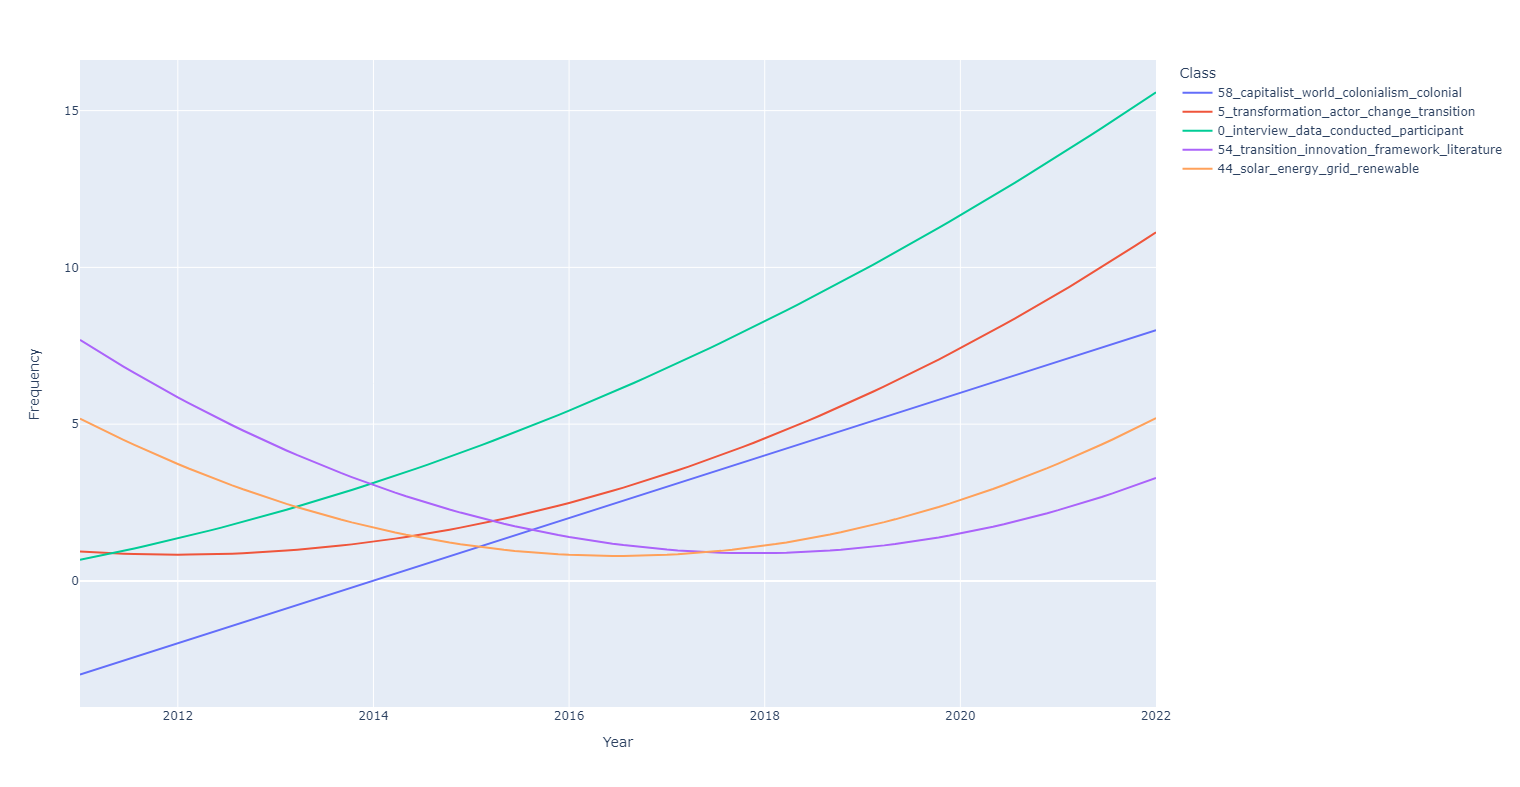
\includegraphics[width=1\linewidth]{images/3j_hot.png}
    \caption{Three Journal Hot Topics}
    \label{fig:enter-label}
\end{figure}
\begin{figure}
    \centering
    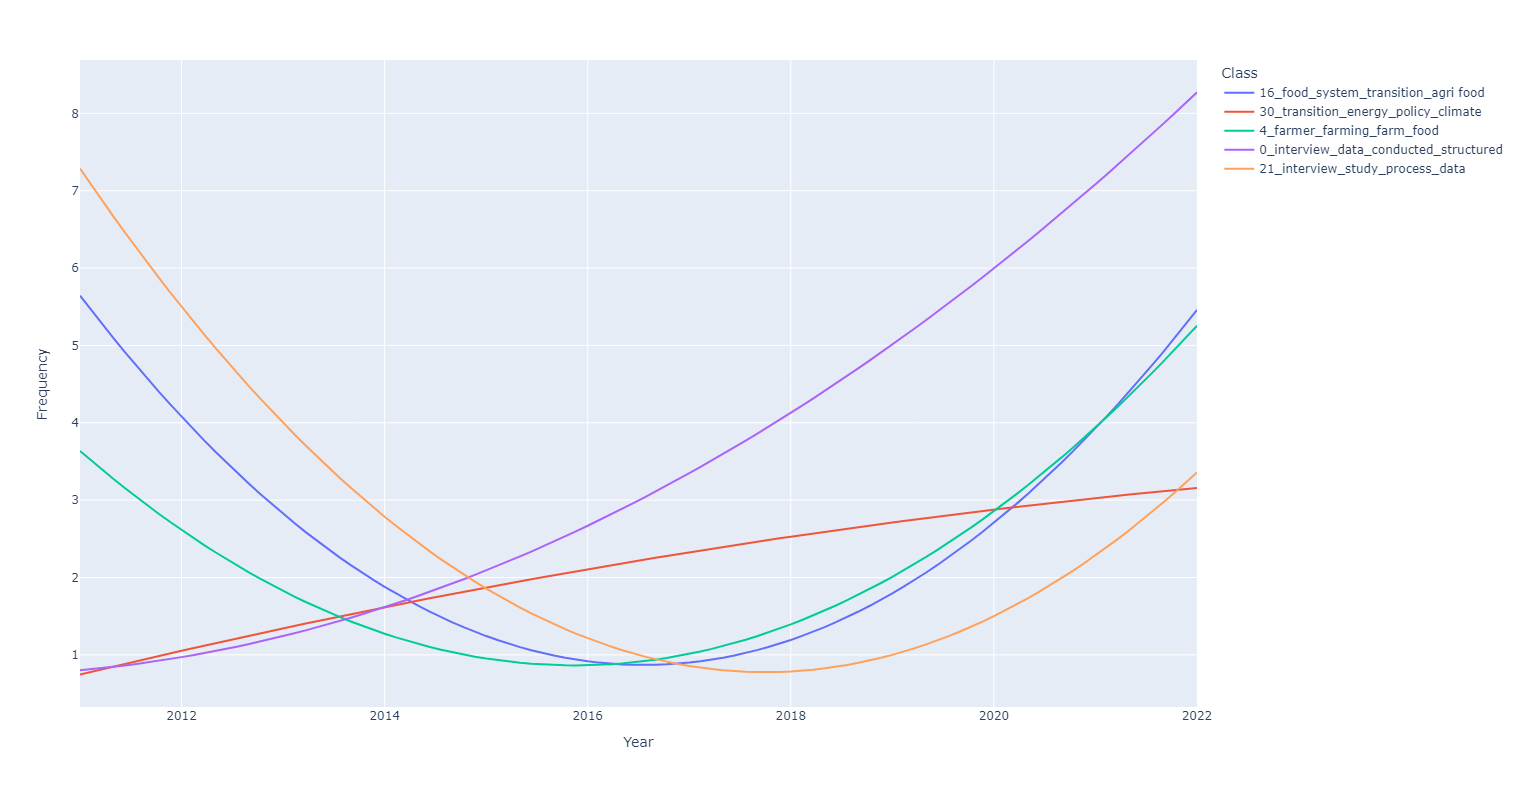
\includegraphics[width=1\linewidth]{images/eist_hot.png}
    \caption{EIST Hot Topics}
    \label{fig:enter-label}
\end{figure}
\begin{figure}
    \centering
    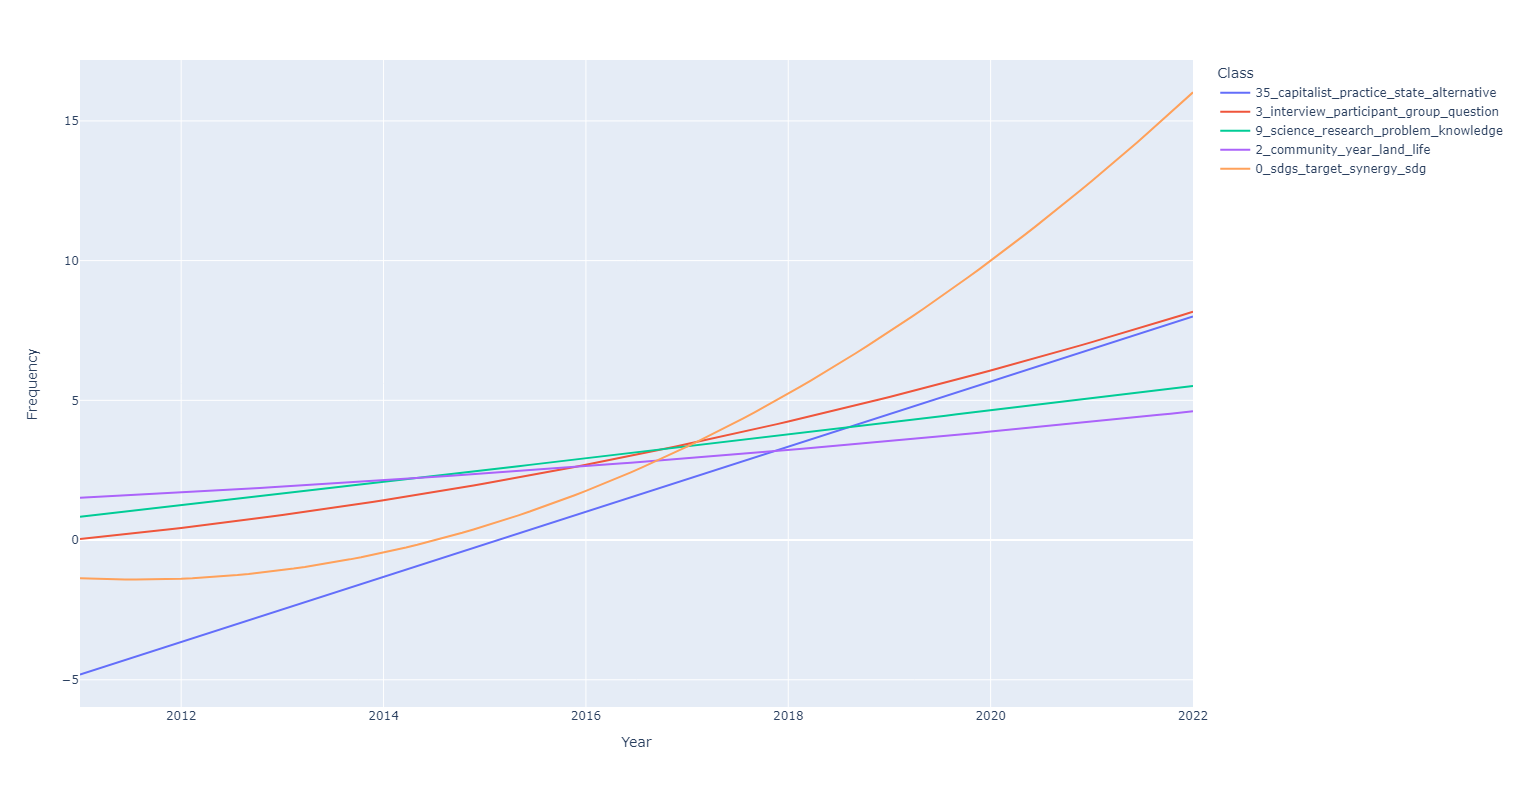
\includegraphics[width=1\linewidth]{images/sussci_hot.png}
    \caption{SUSSCI Hot Topics}
    \label{fig:enter-label}
\end{figure}
\begin{figure}
    \centering
    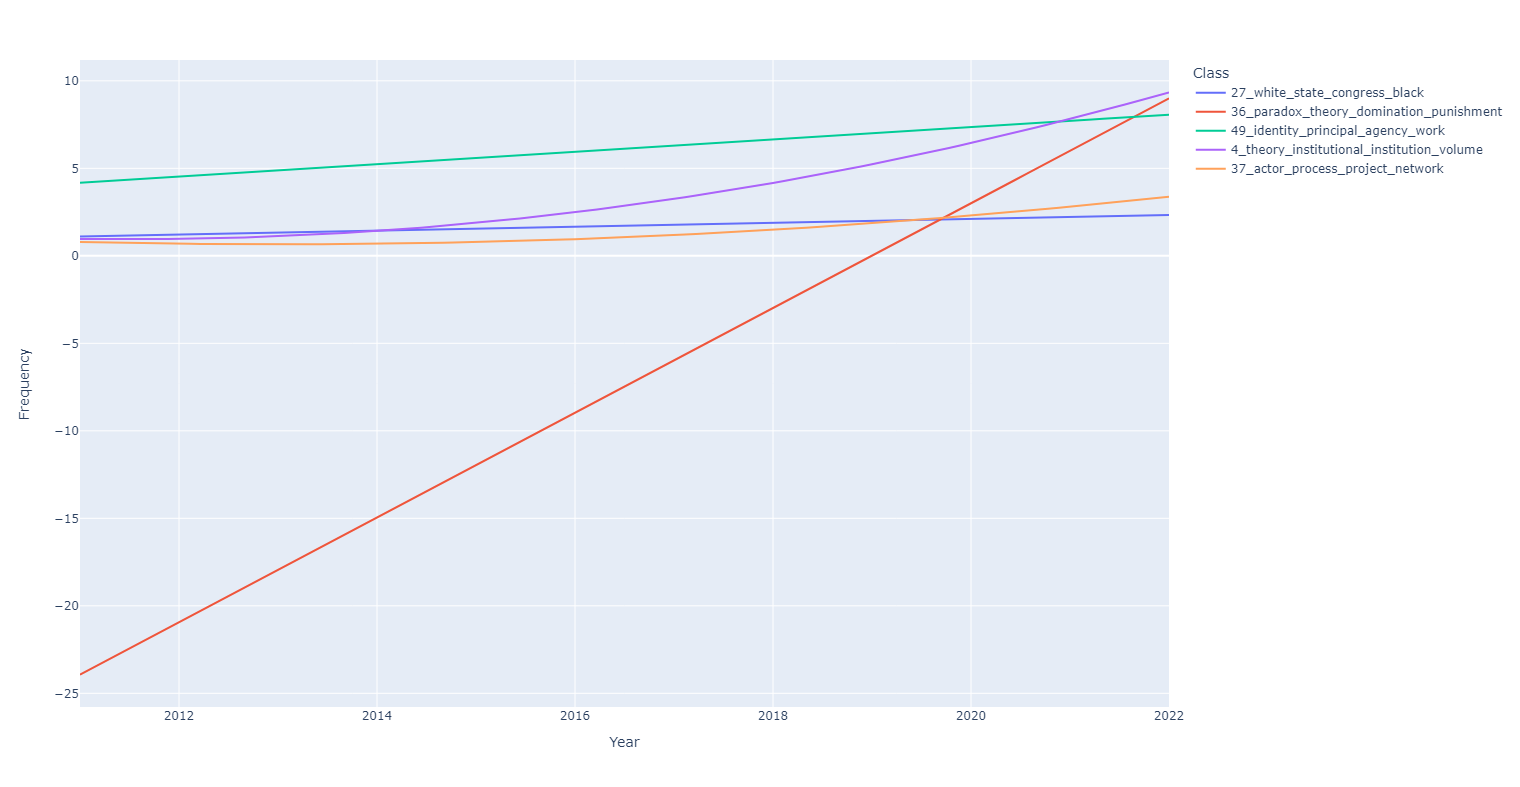
\includegraphics[width=1\linewidth]{images/rsog_hot.png}
    \caption{RSOG Hot Topics}
    \label{fig:enter-label}
\end{figure}
\begin{figure}
    \centering
    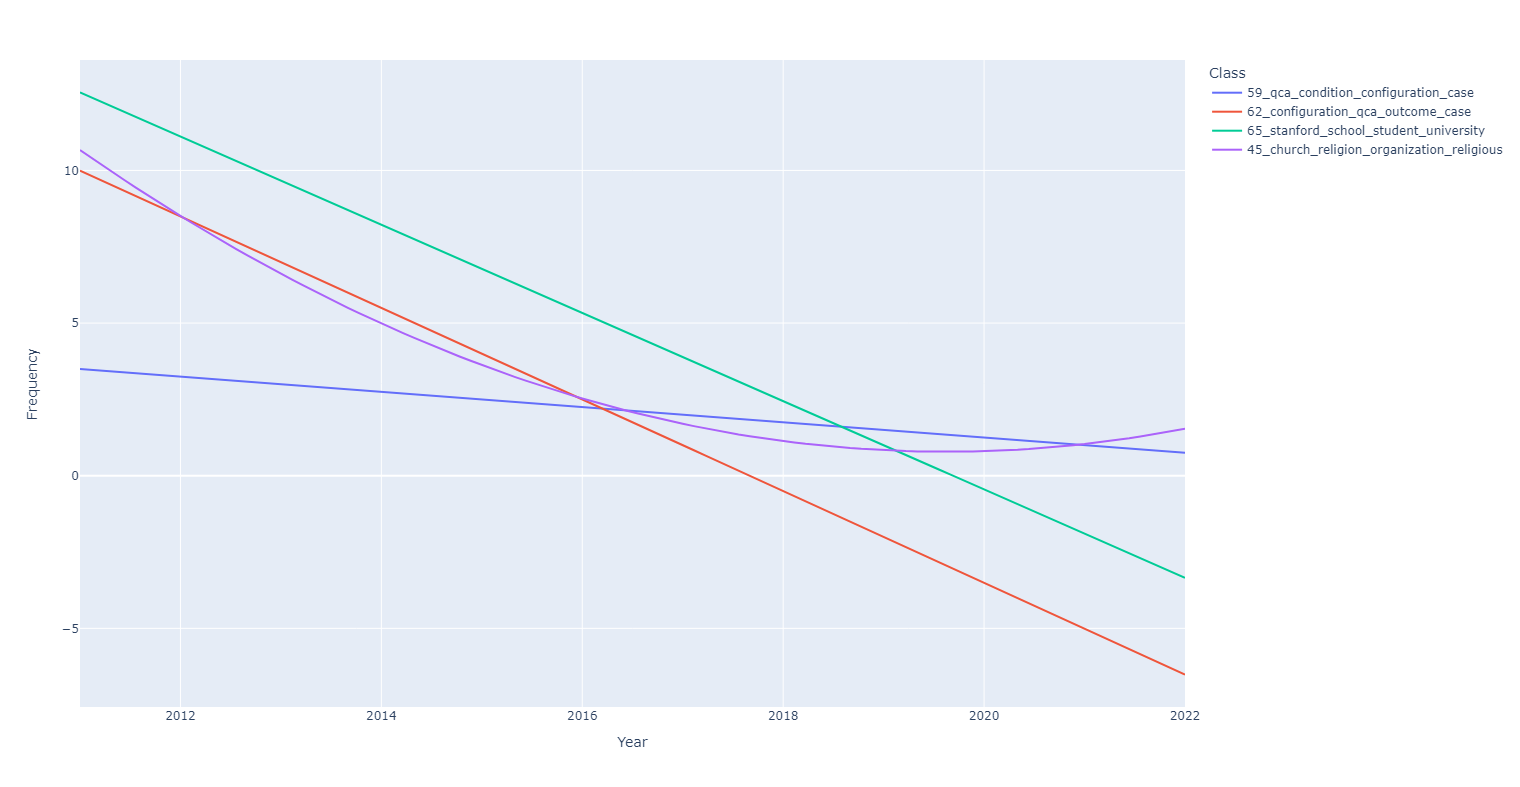
\includegraphics[width=1\linewidth]{images/3j_cold.png}
    \caption{Three Journal Cold Topics}
    \label{fig:enter-label}
\end{figure}
\begin{figure}
    \centering
    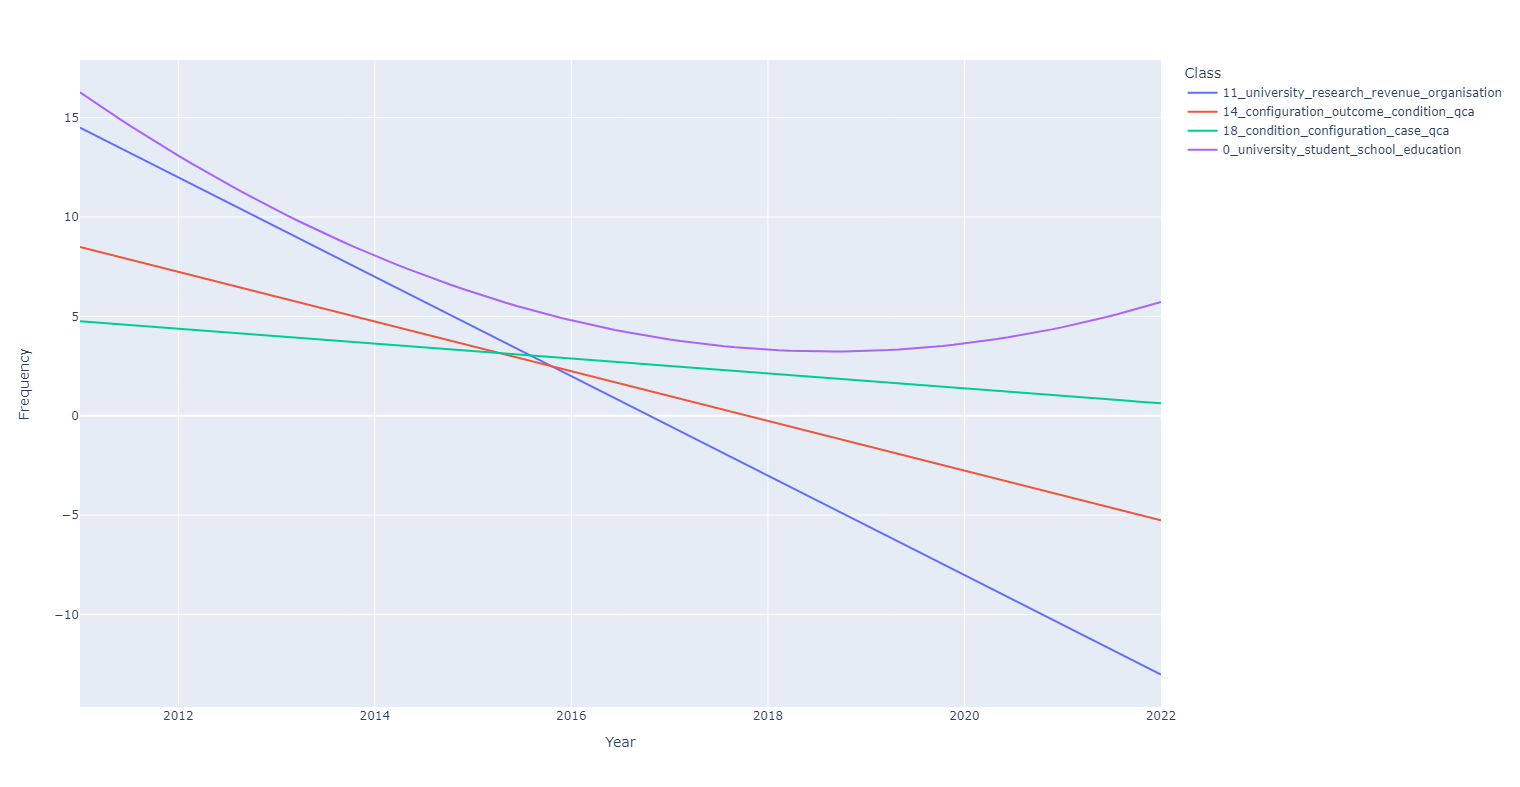
\includegraphics[width=1\linewidth]{images/rsog_cold.png}
    \caption{RSOG COld Topics}
    \label{fig:enter-label}
\end{figure}

%\subsubsection{Wallflower Topics}
\begin{figure}
    \centering
    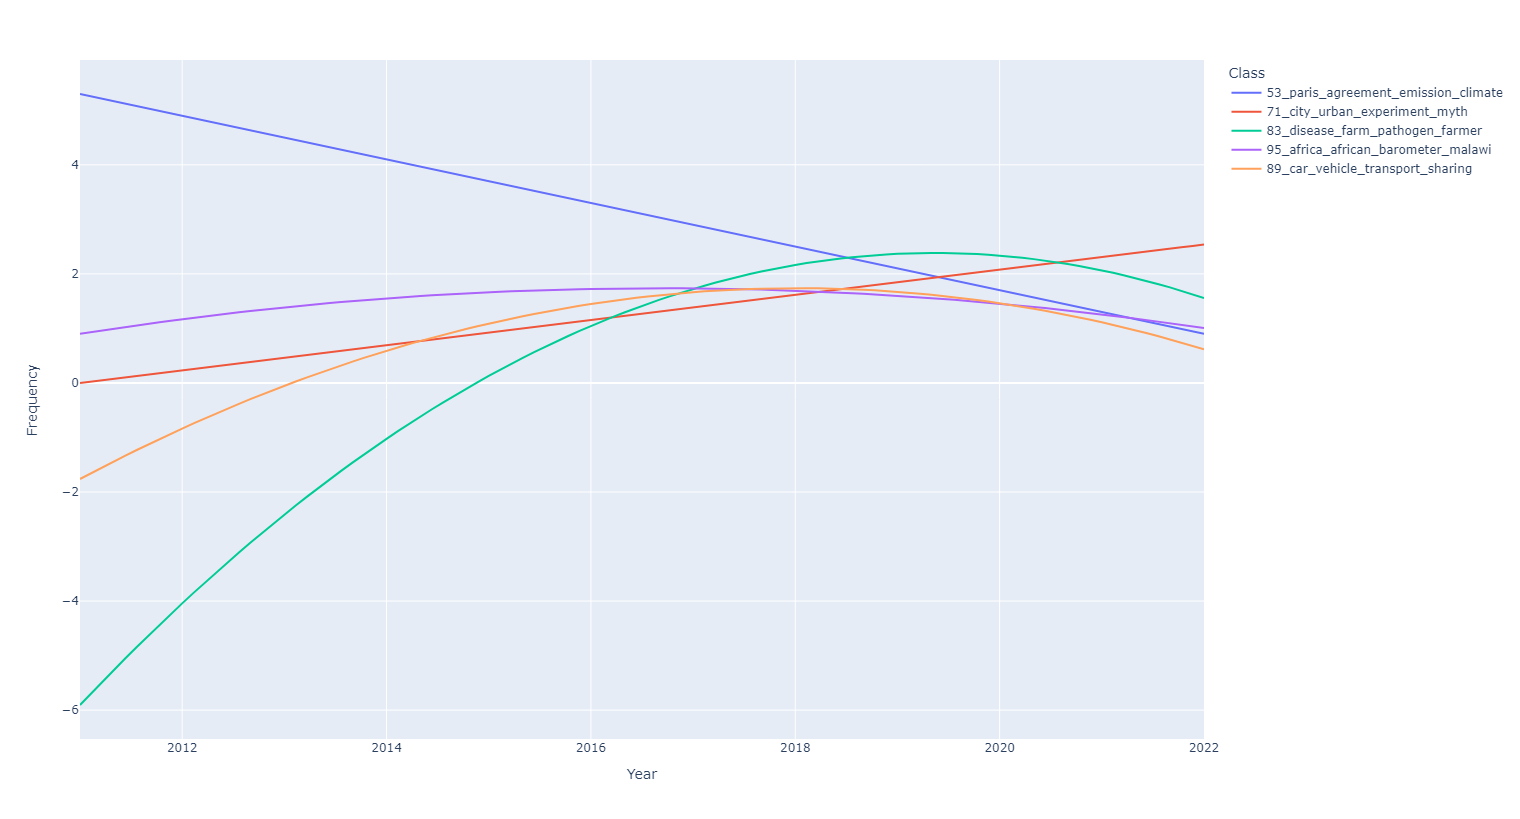
\includegraphics[width=1\linewidth]{images/3j_wallflower.png}
    \caption{Three Journal Wallflower Topics}
    \label{fig:enter-label}
\end{figure}
\begin{figure}
    \centering
    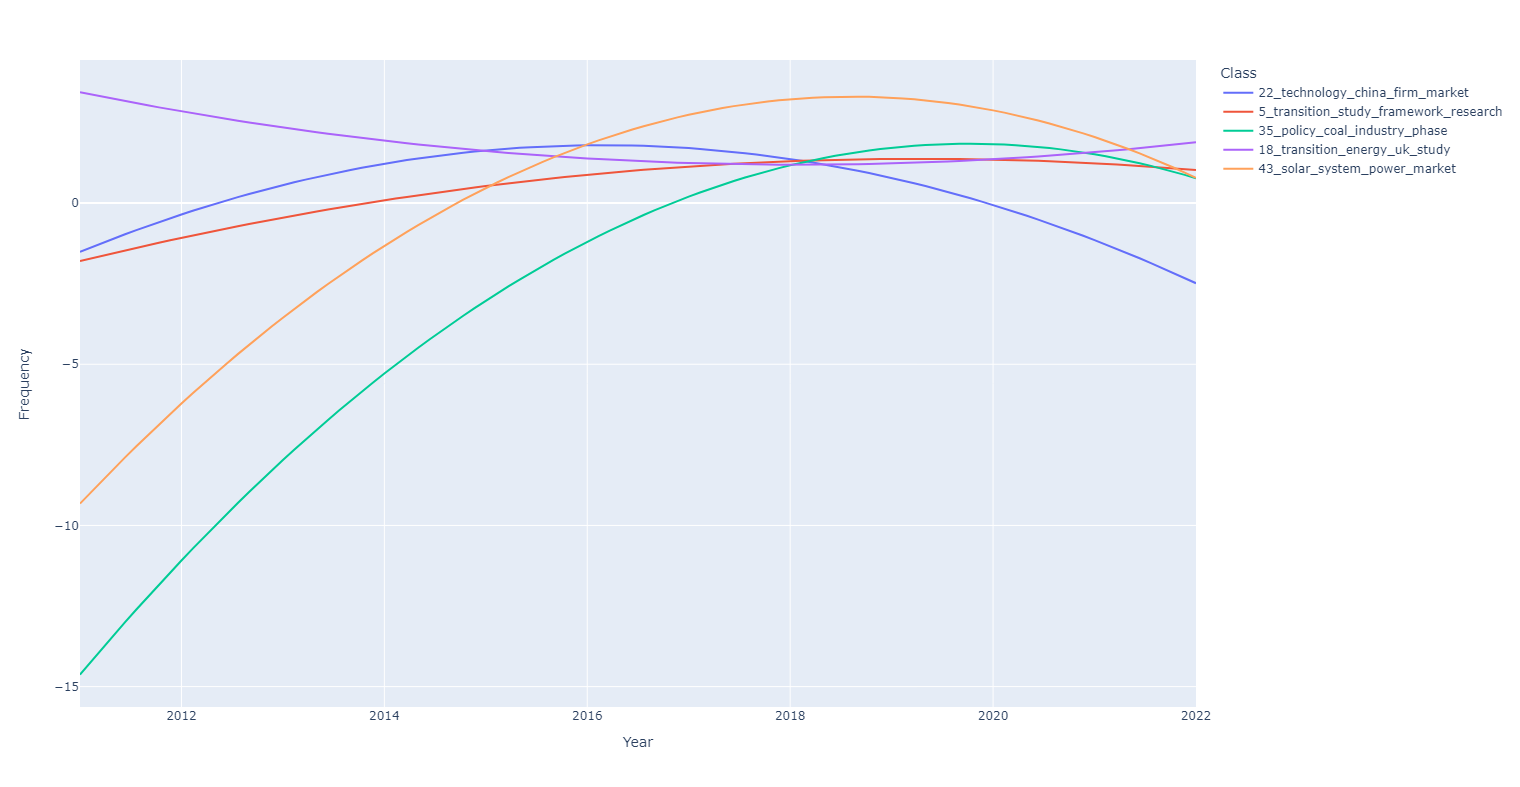
\includegraphics[width=1\linewidth]{images/eist_wallflower.png}
    \caption{EIST Wallflower Topics}
    \label{fig:enter-label}
\end{figure}
\begin{figure}
    \centering
    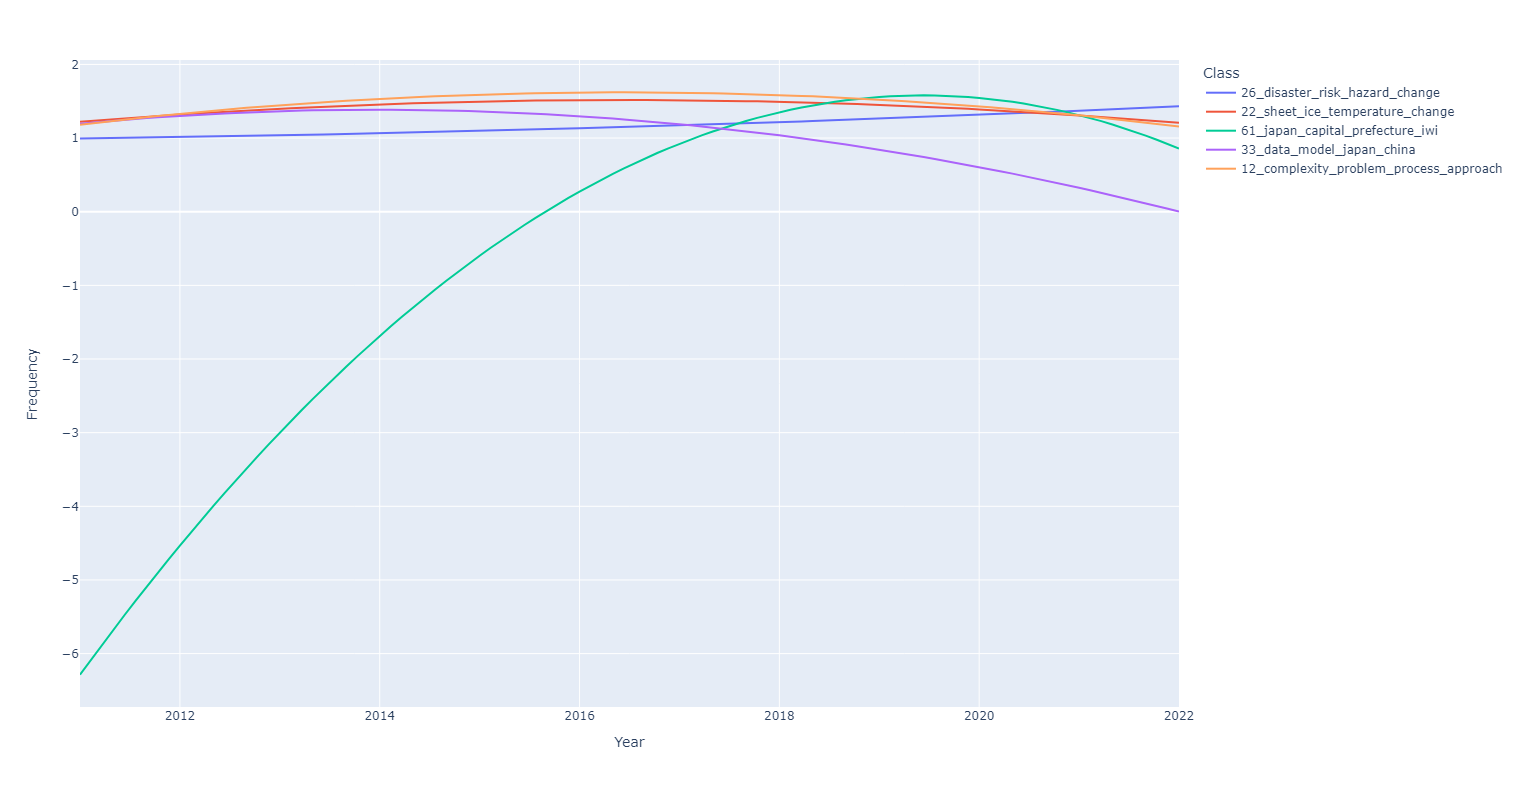
\includegraphics[width=1\linewidth]{images/sussci_wallflower.png}
    \caption{SUSSCI Wallflower Topics}
    \label{fig:enter-label}
\end{figure}
\begin{figure}
    \centering
    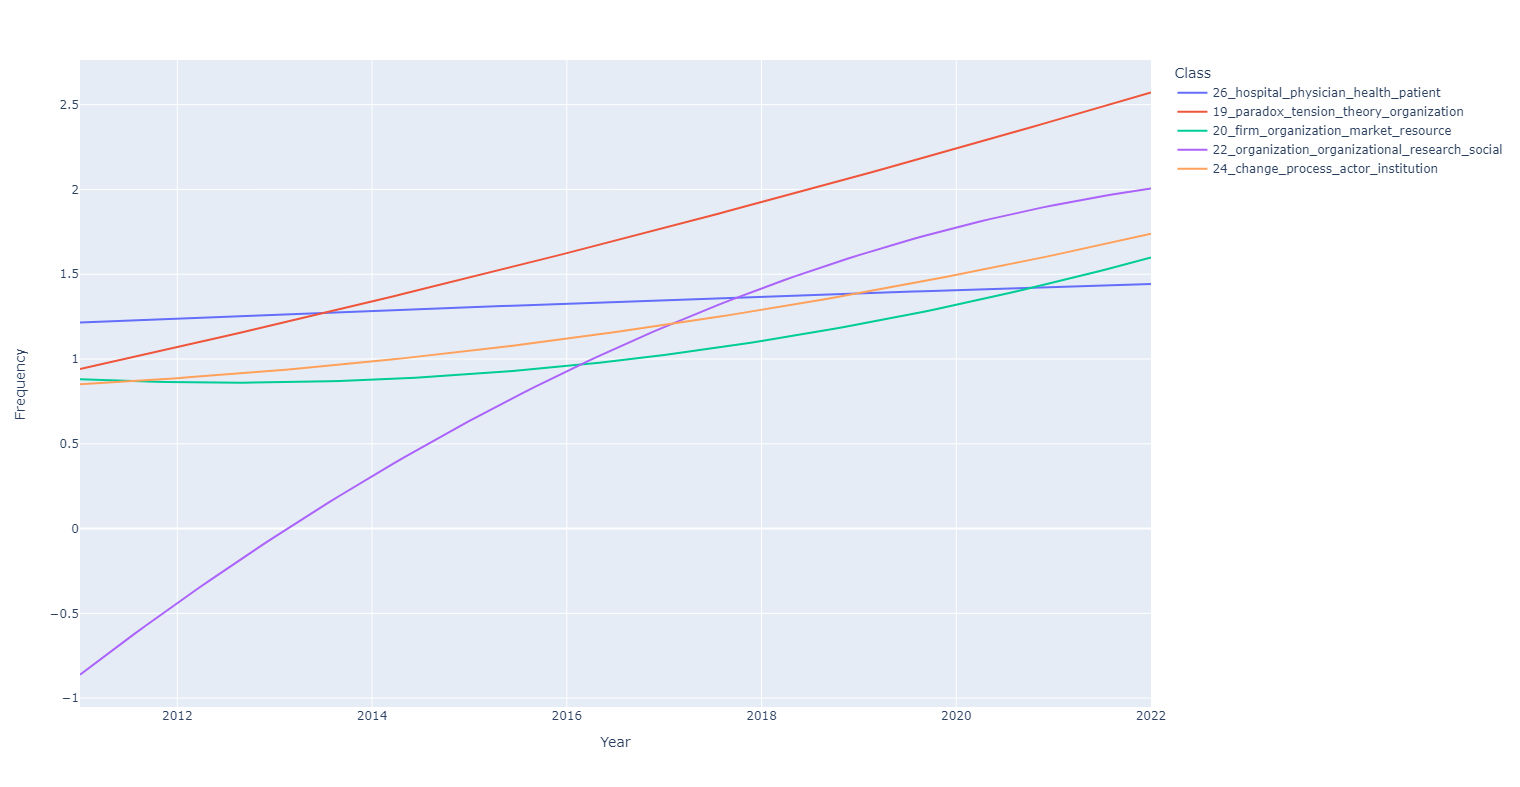
\includegraphics[width=1\linewidth]{images/rsog_wallflower.png}
    \caption{RSOG Wallflower Topics}
    \label{fig:enter-label}
\end{figure}

%\subsubsection{Evergreen Topics}
\begin{figure}
    \centering
    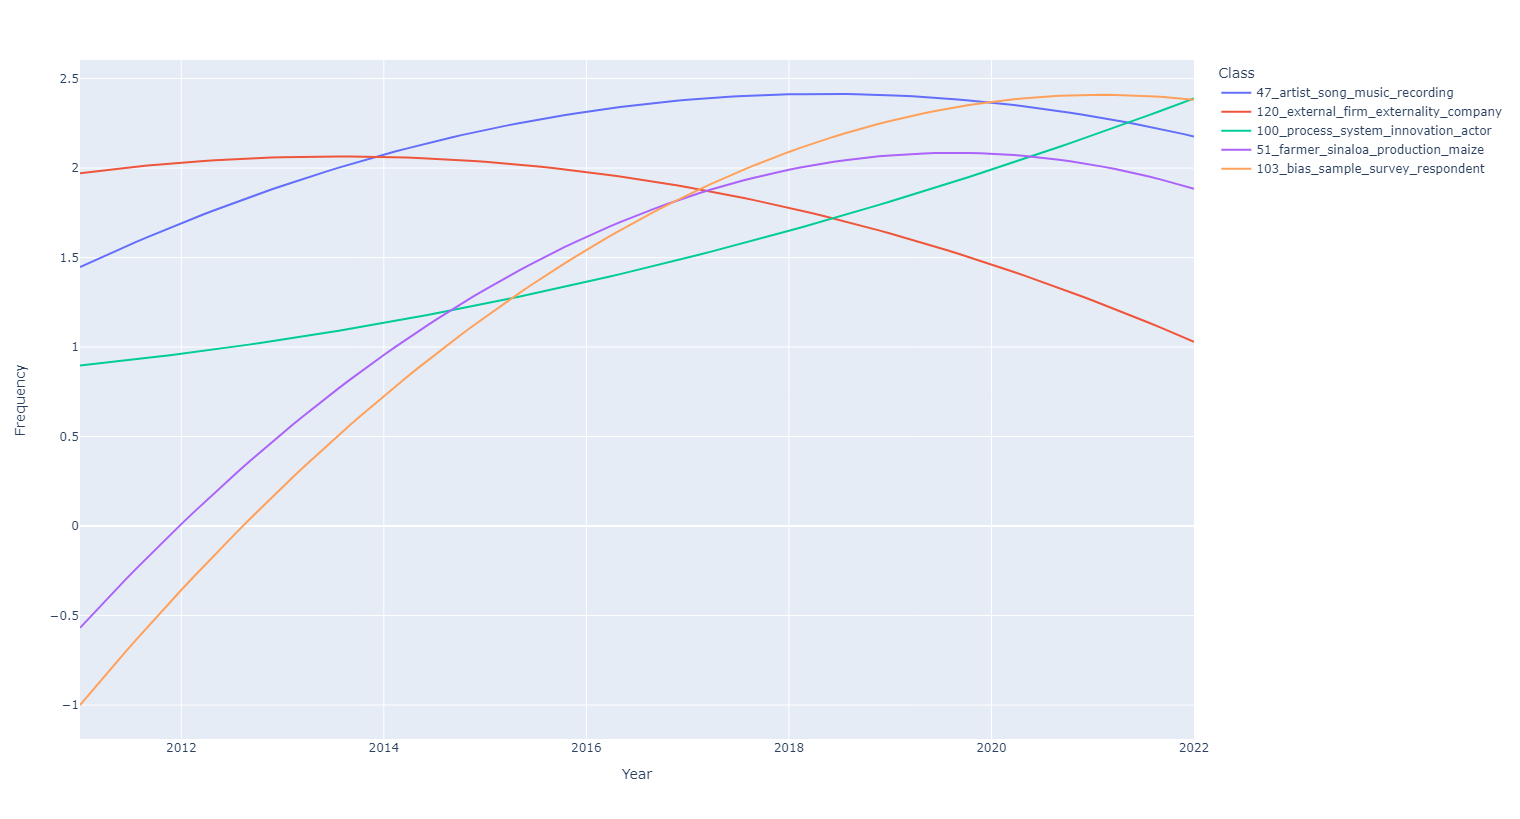
\includegraphics[width=1\linewidth]{images/3j_evergreen.png}
    \caption{Three Journal Evergreen Topics}
    \label{fig:enter-label}
\end{figure}
\begin{figure}
    \centering
    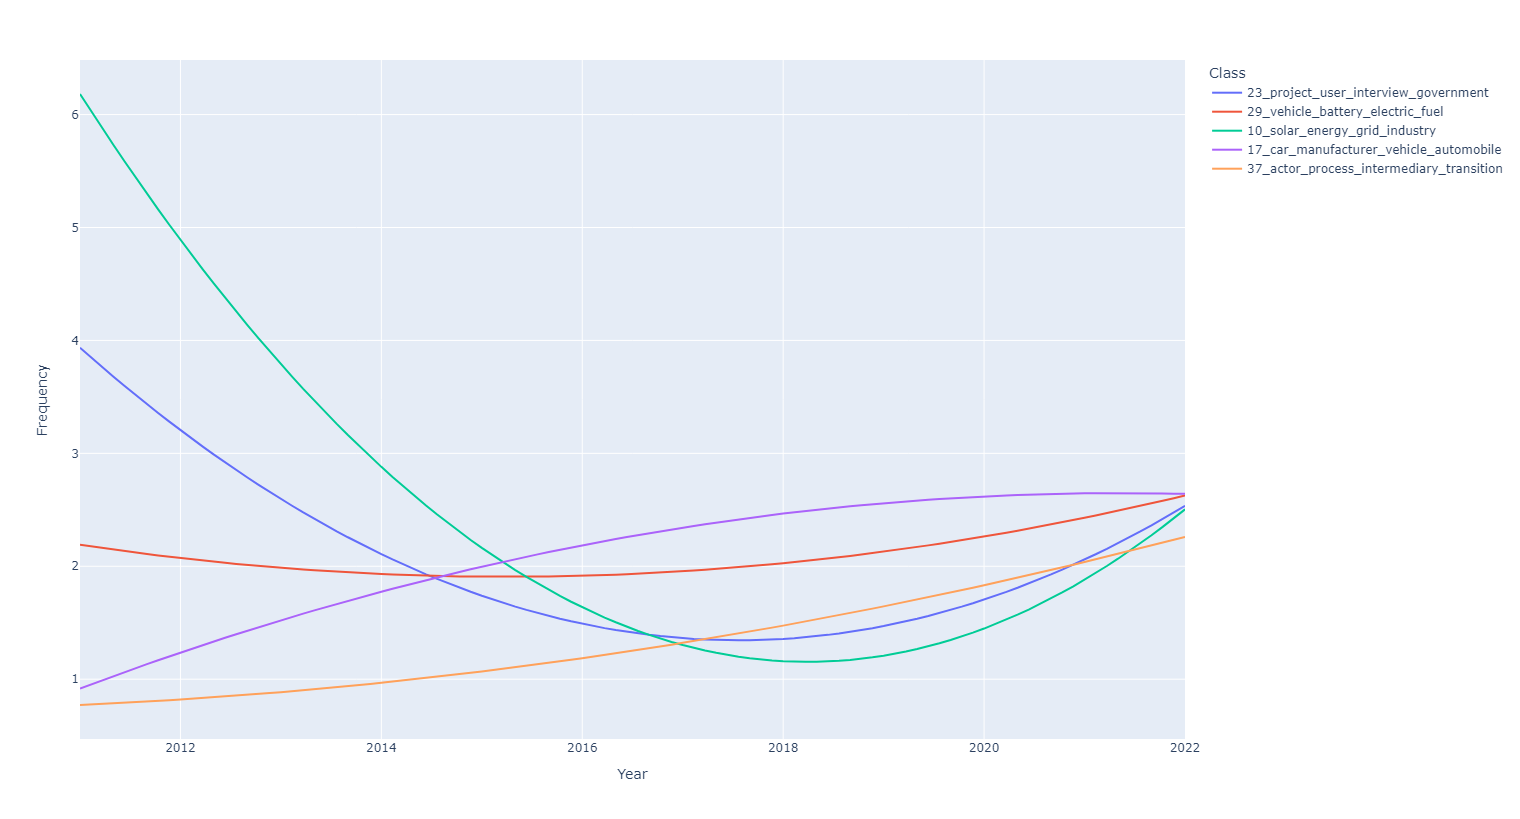
\includegraphics[width=1\linewidth]{images/eist_evergreen.png}
    \caption{EIST Evergreen Topics}
    \label{fig:enter-label}
\end{figure}
\begin{figure}
    \centering
    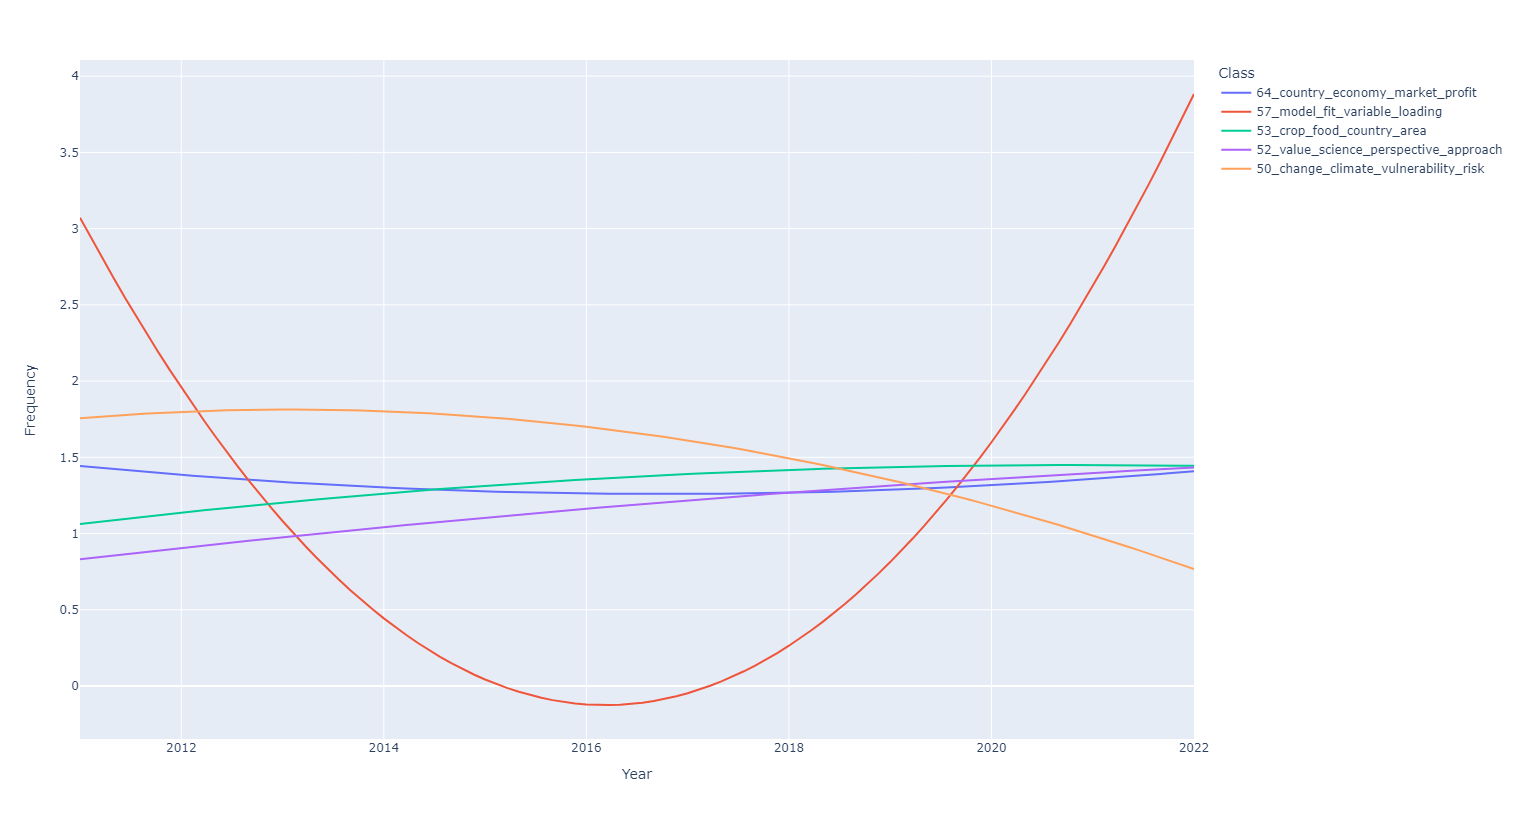
\includegraphics[width=1\linewidth]{images/sussci_evergreen.png}
    \caption{SUSSCI Evergreen Topics}
    \label{fig:enter-label}
\end{figure}
\begin{figure}
    \centering
    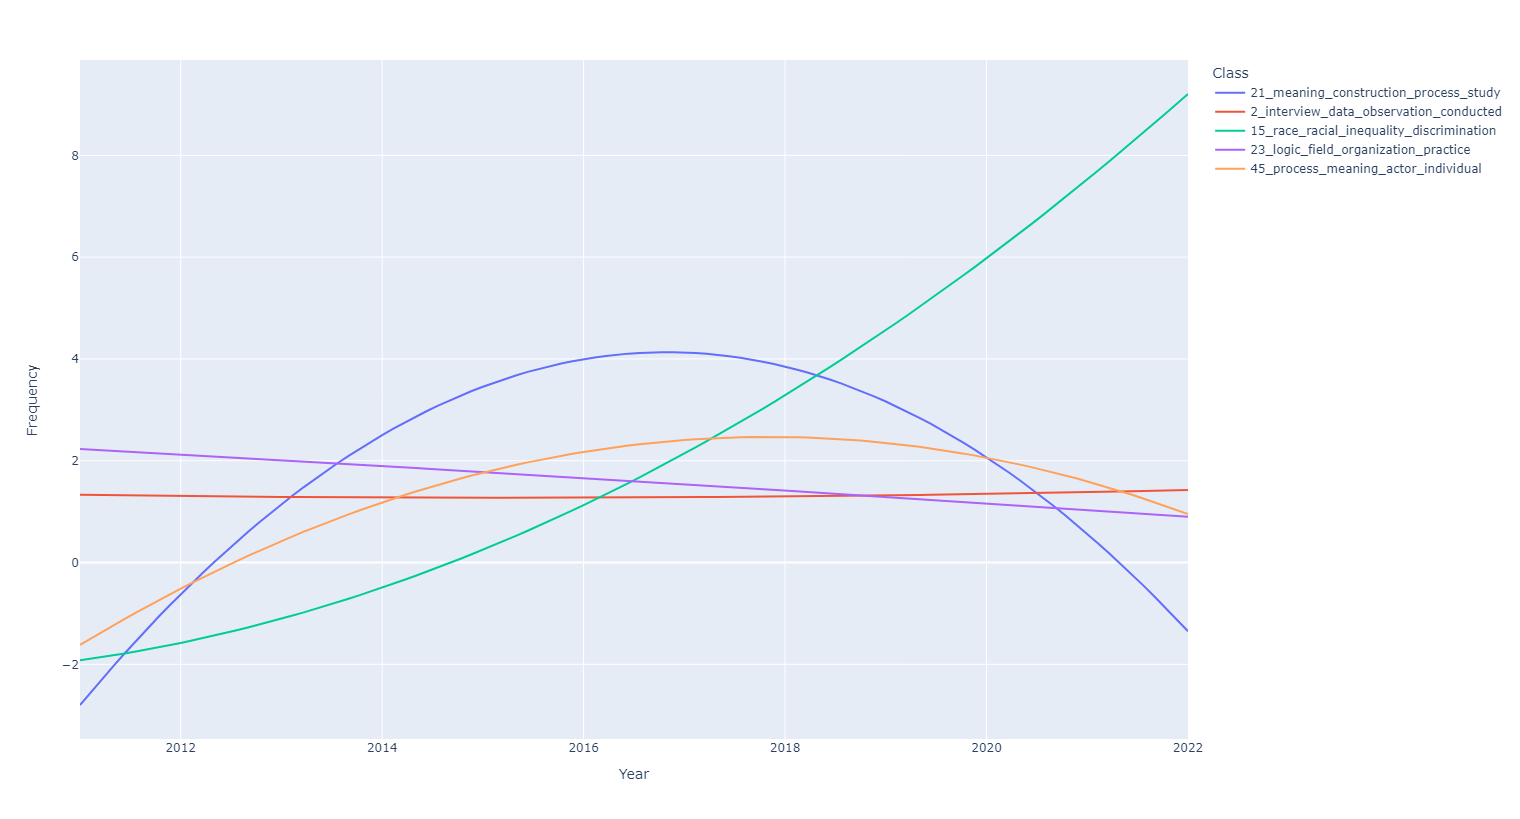
\includegraphics[width=1\linewidth]{images/rsog_evergreen.png}
    \caption{RSOG Evergreen Topics}
    \label{fig:enter-label}
\end{figure}

%\subsubsection{Revival Topics}
\begin{figure}
    \centering
    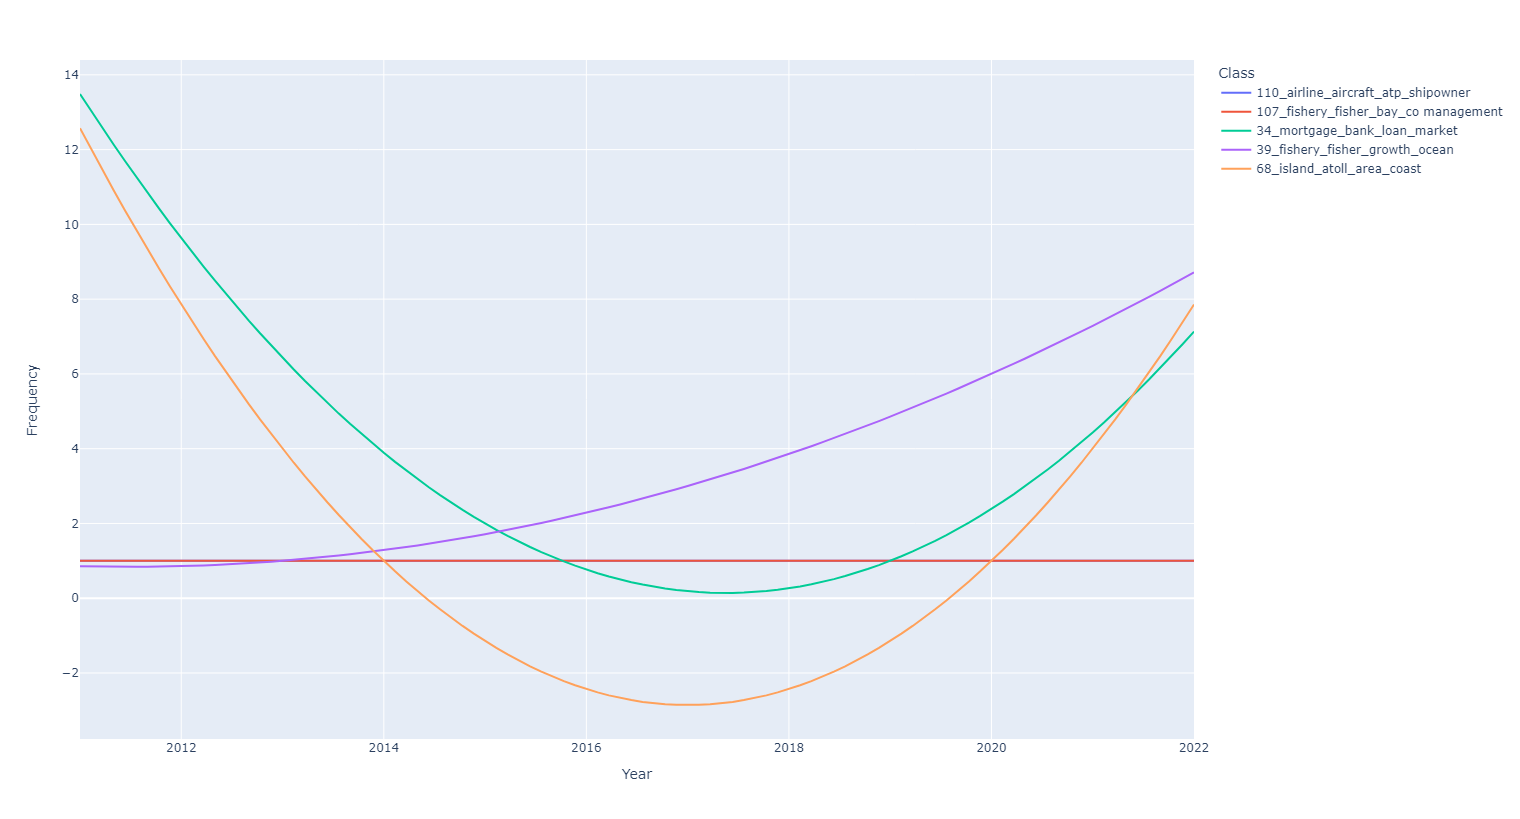
\includegraphics[width=1\linewidth]{images/3j_reviving.png}
    \caption{Three Journal Reviving Topics}
    \label{fig:enter-label}
\end{figure}
\begin{figure}
    \centering
    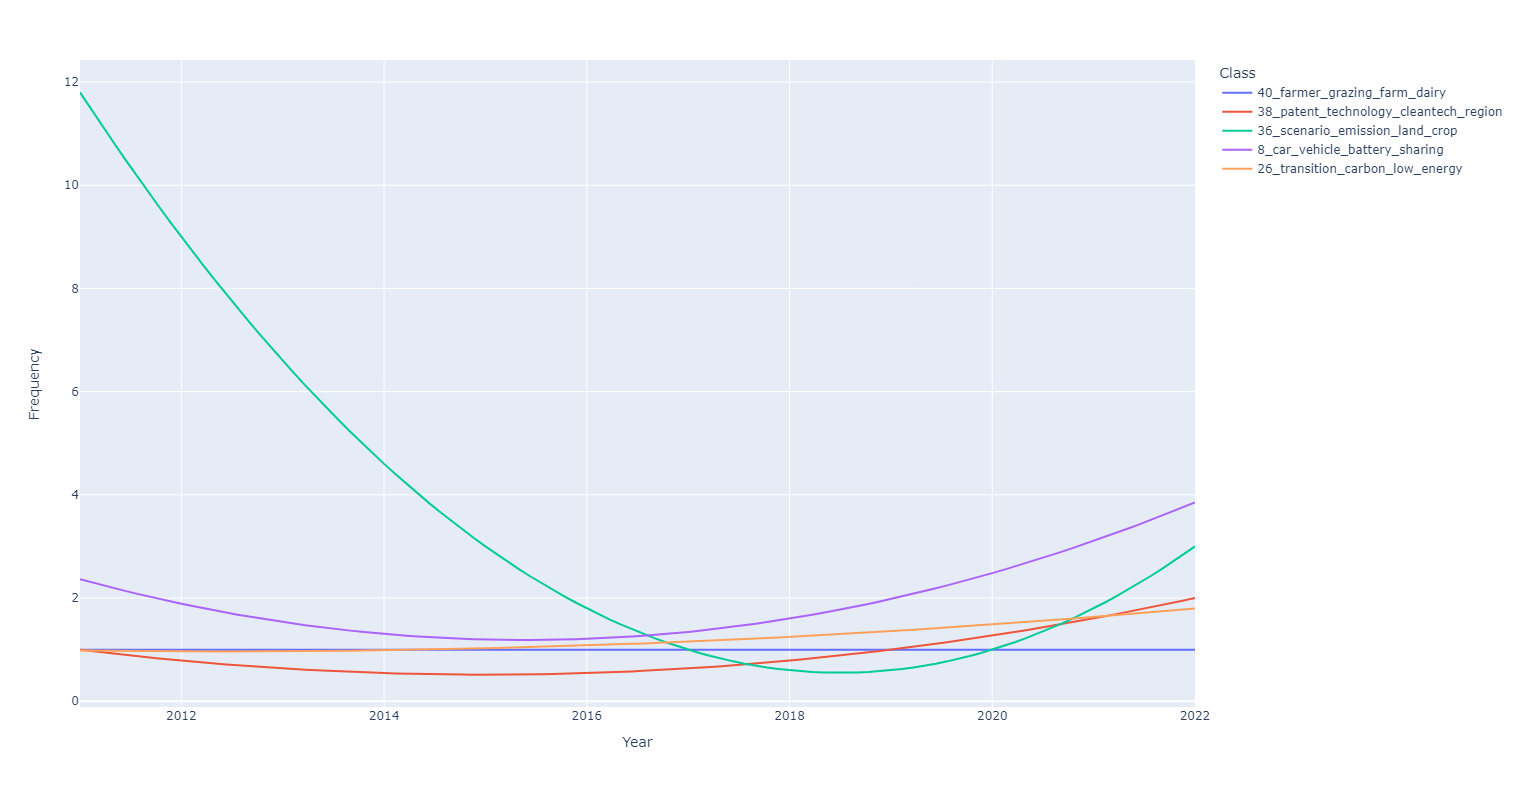
\includegraphics[width=1\linewidth]{images/eist_reviving.png}
    \caption{EIST Reviving Topics}
    \label{fig:enter-label}
\end{figure}
\begin{figure}
    \centering
    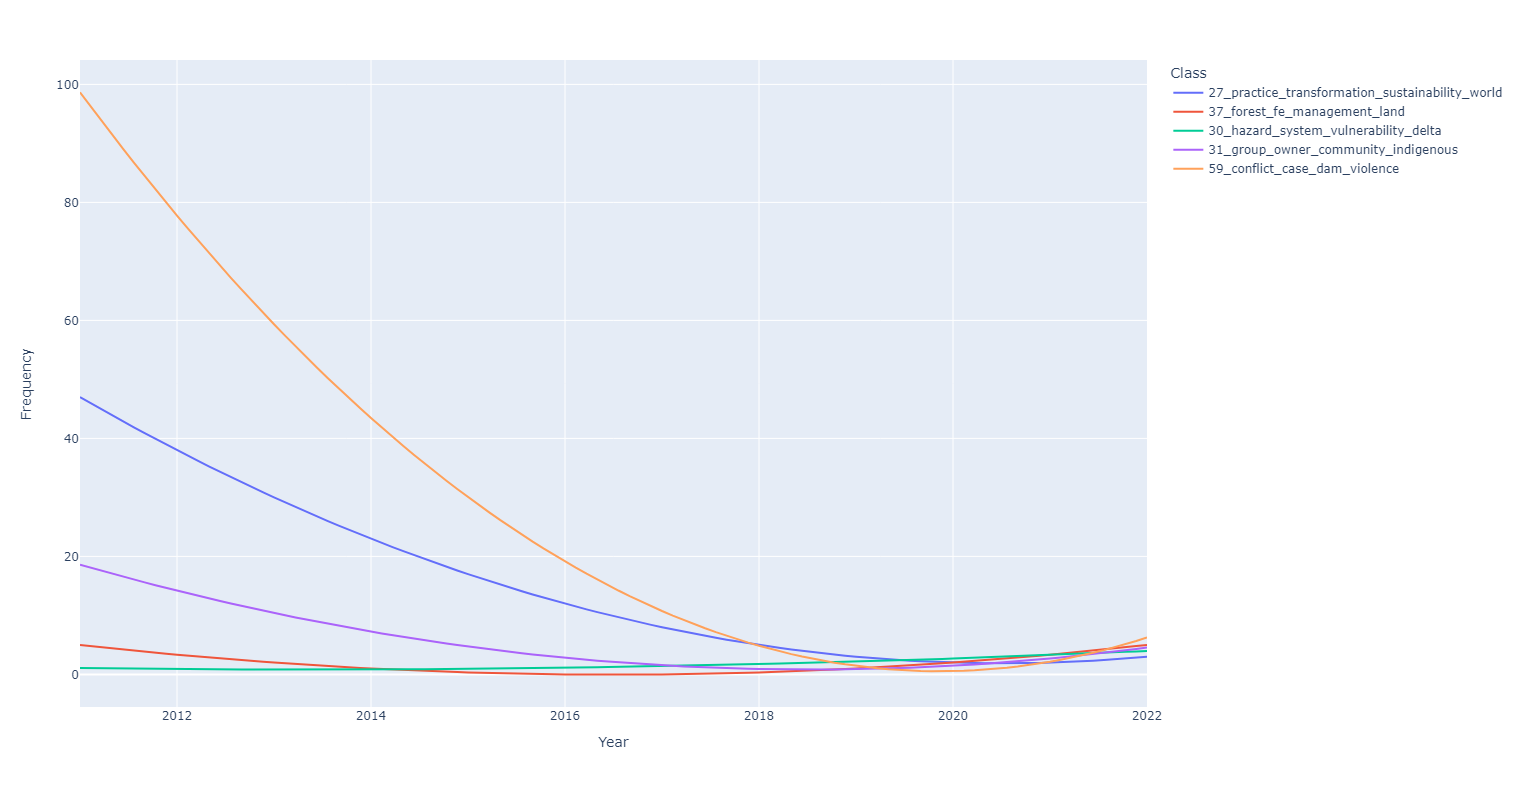
\includegraphics[width=1\linewidth]{images/sussci_reviving.png}
    \caption{SUSSCI Reviving Topics}
    \label{fig:enter-label}
\end{figure}
\begin{figure}
    \centering
    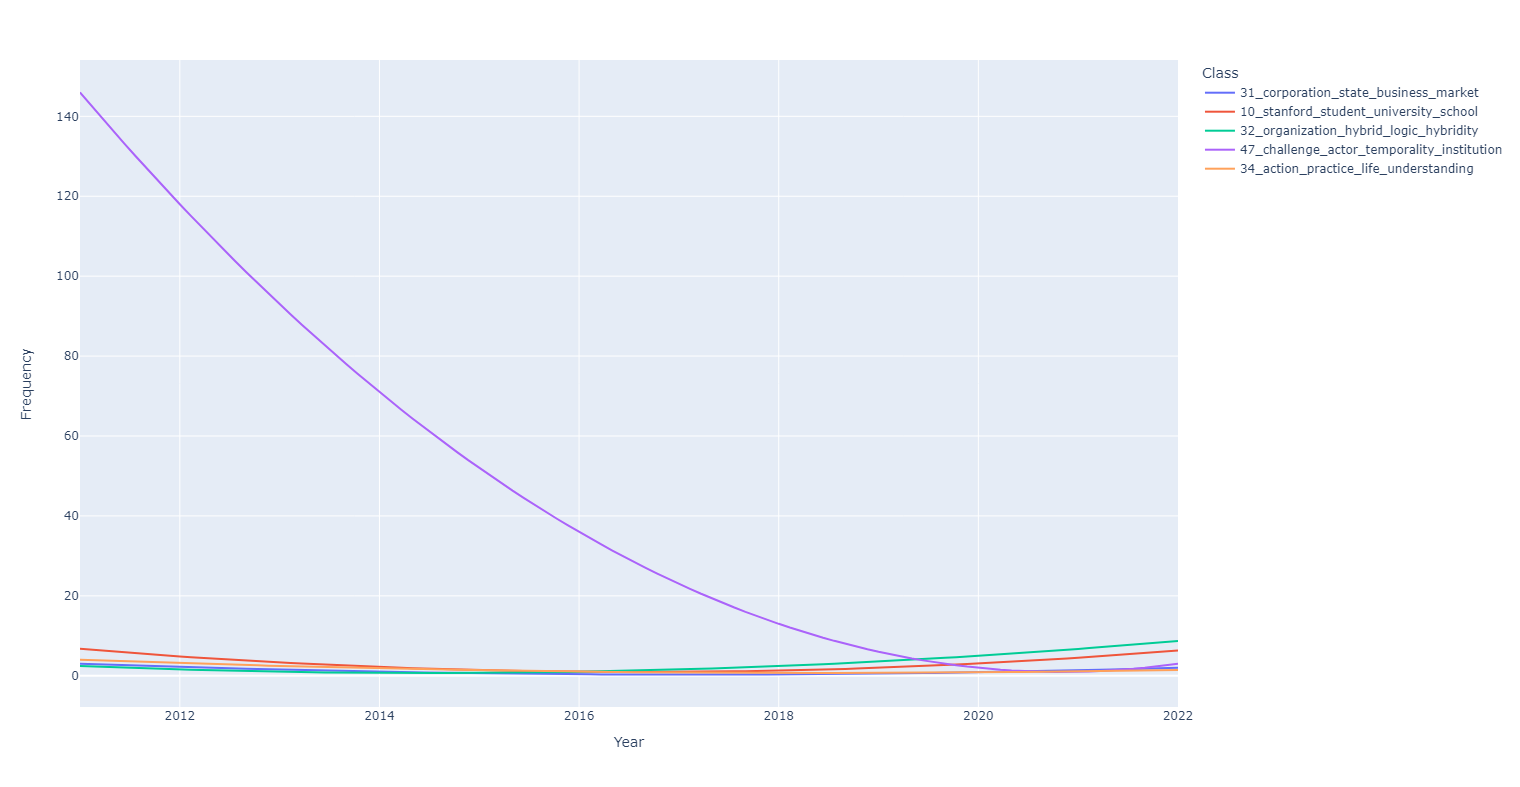
\includegraphics[width=1\linewidth]{images/rsog_reviving.png}
    \caption{RSOG Reviving Topics}
    \label{fig:enter-label}
\end{figure}
\onecolumn
\begin{figure}
    \centering
    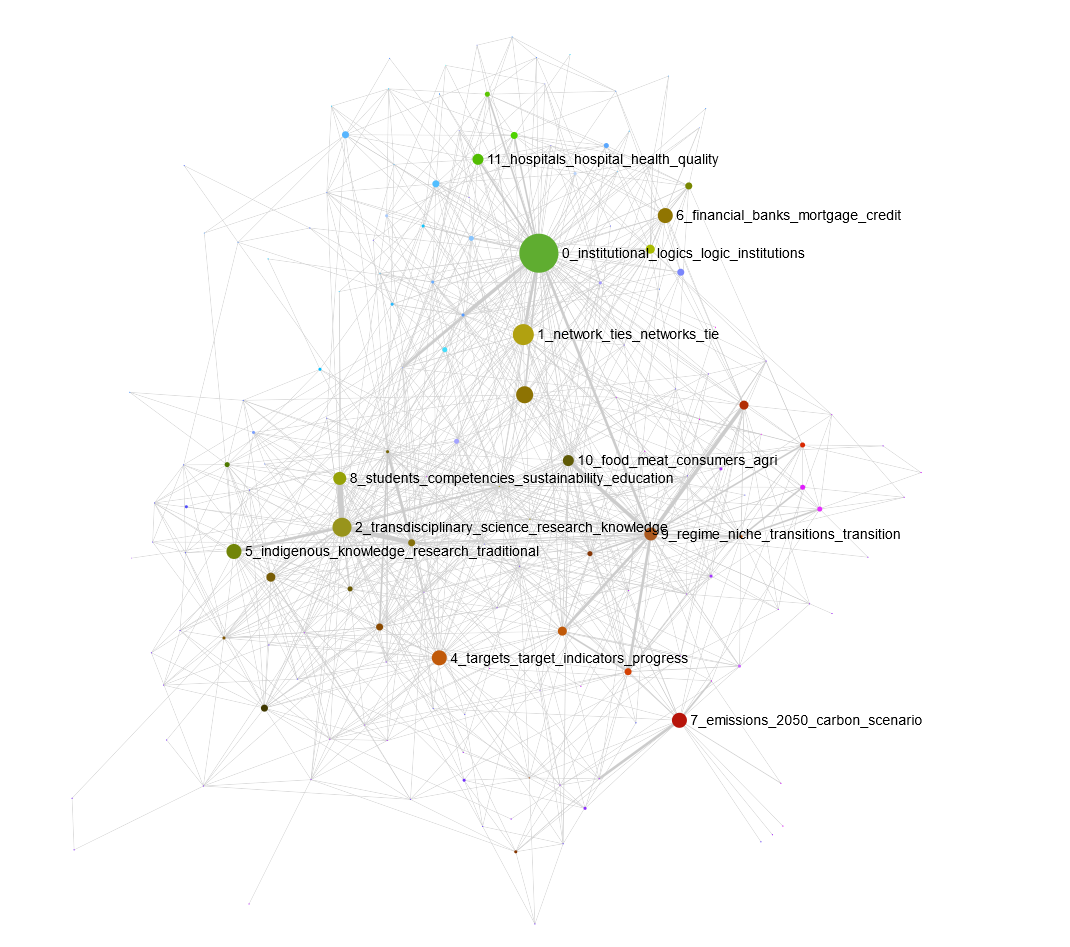
\includegraphics[width=1\linewidth]{images/all_topic_network.png}
    \caption{Three Journal Topic Network - High level}
    \label{fig:enter-label}
\end{figure}
\begin{figure}
    \centering
    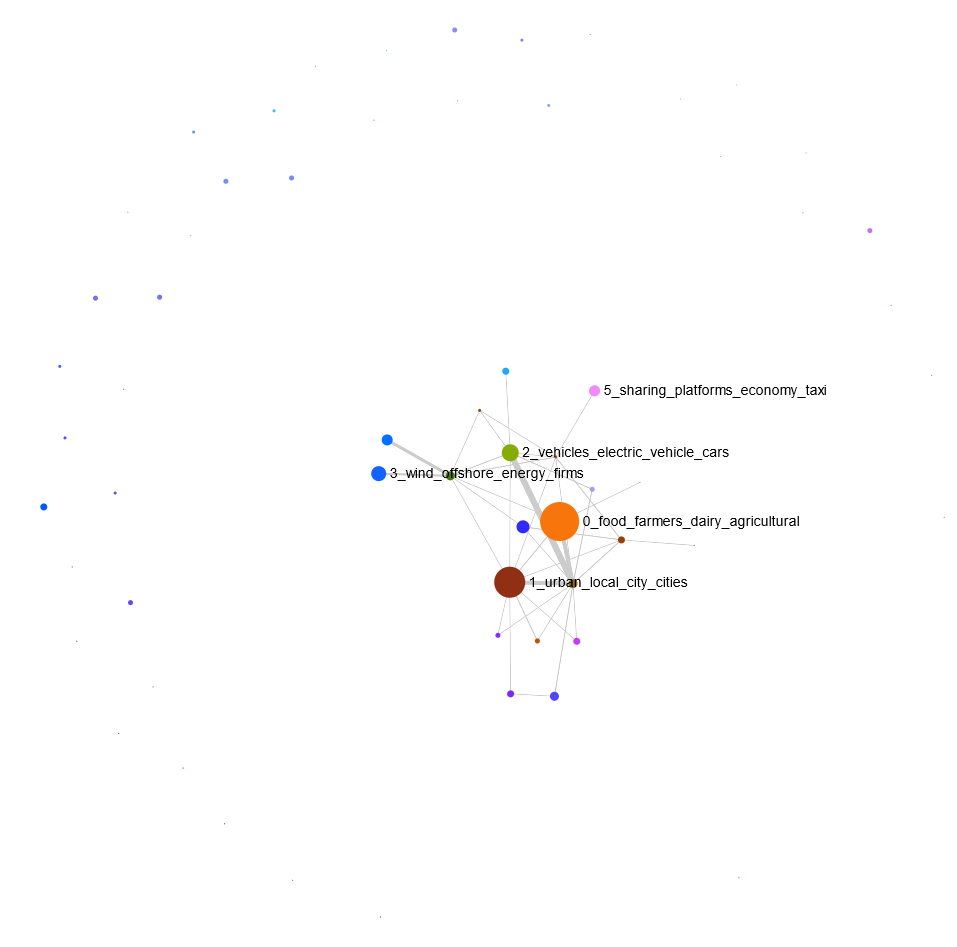
\includegraphics[width=0.5\linewidth]{images/eist_topic_network_3+.png}
    \caption{EIST Topic Network (Weight 3)}
    \label{fig:enter-label}
\end{figure}
\begin{figure}
    \centering
    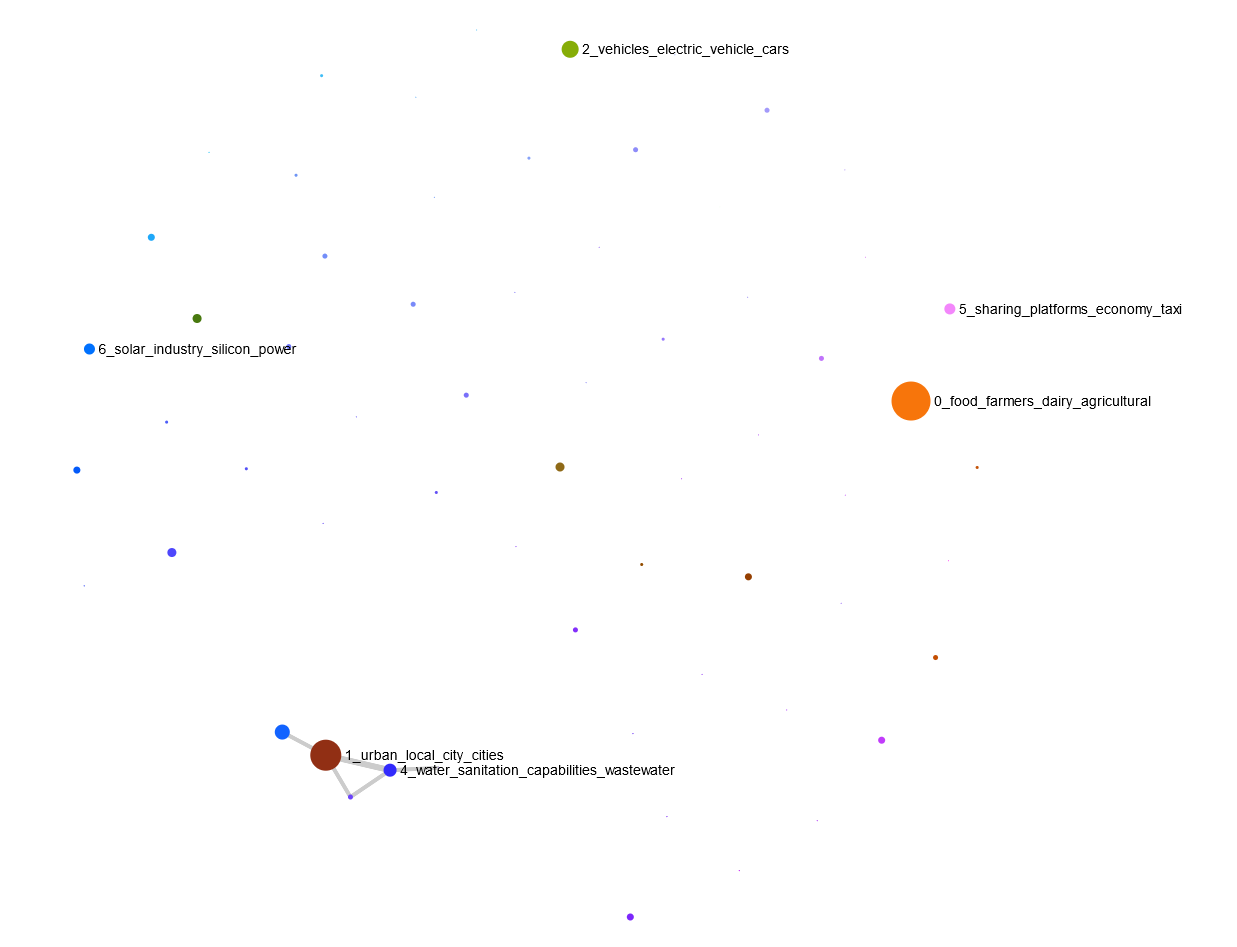
\includegraphics[width=0.7\linewidth]{images/eist_topic_network_5+.png}
    \caption{EIST Topic Network (Weight 5 or more)}
    \label{fig:enter-label}
\end{figure}
\begin{figure}
    \centering
    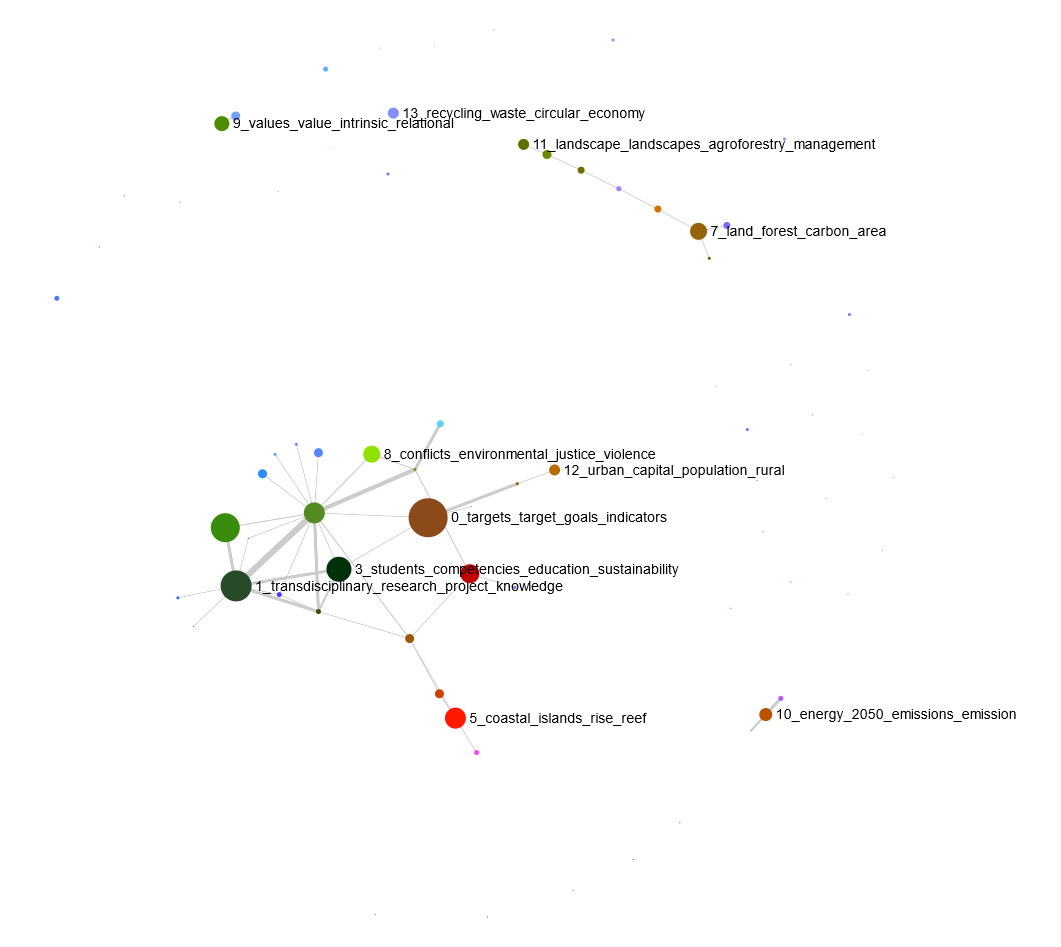
\includegraphics[width=0.7\linewidth]{images/ss_topic_network_3+.png}
    \caption{SUSSCI Topic Network (Weight 3)Enter Caption}
    \label{fig:enter-label}
\end{figure}
\begin{figure}
    \centering
    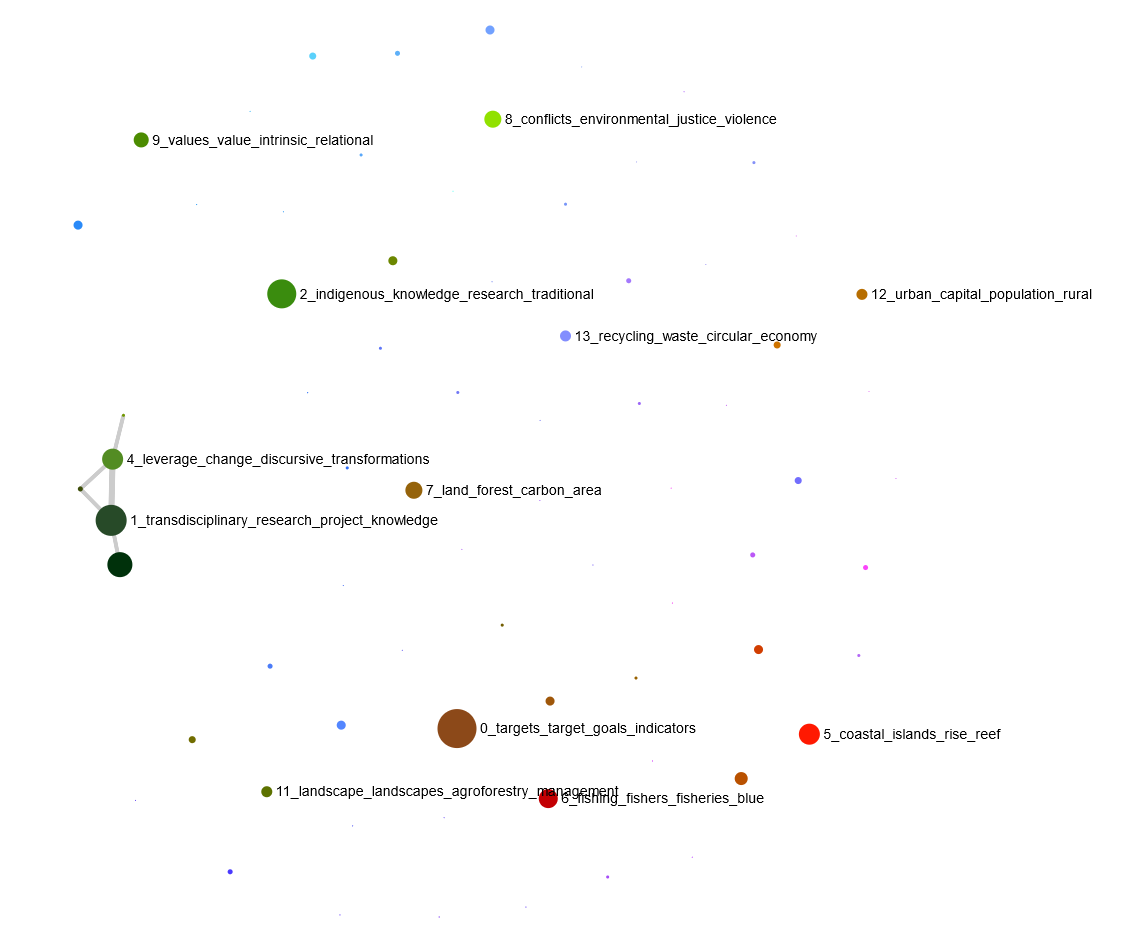
\includegraphics[width=0.7\linewidth]{images/ss_topic_network_5+.png}
    \caption{SUSSCI Topic Network (Weight 5 or more)}
    \label{fig:enter-label}
\end{figure}
\begin{figure}
    \centering
    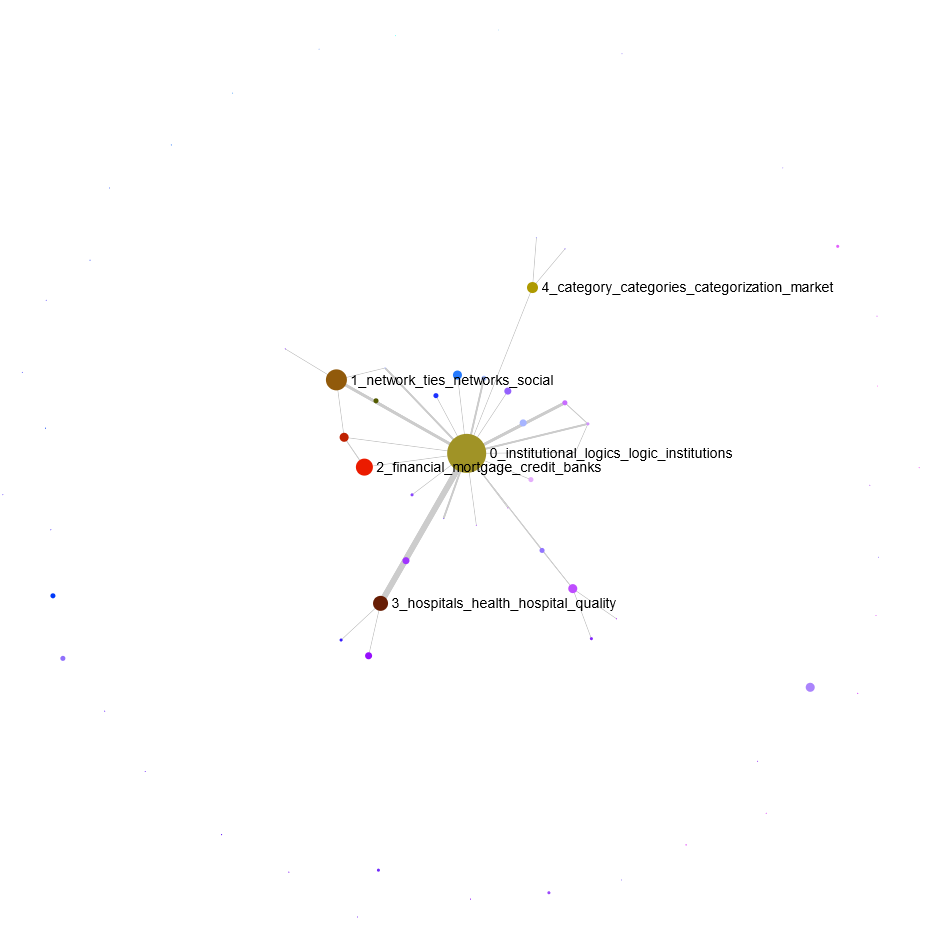
\includegraphics[width=0.7\linewidth]{images/rsog_topic_network_3+.png}
    \caption{RSOG Topic Network (Weight 3)}
    \label{fig:enter-label}
\end{figure}
\begin{figure}
    \centering
    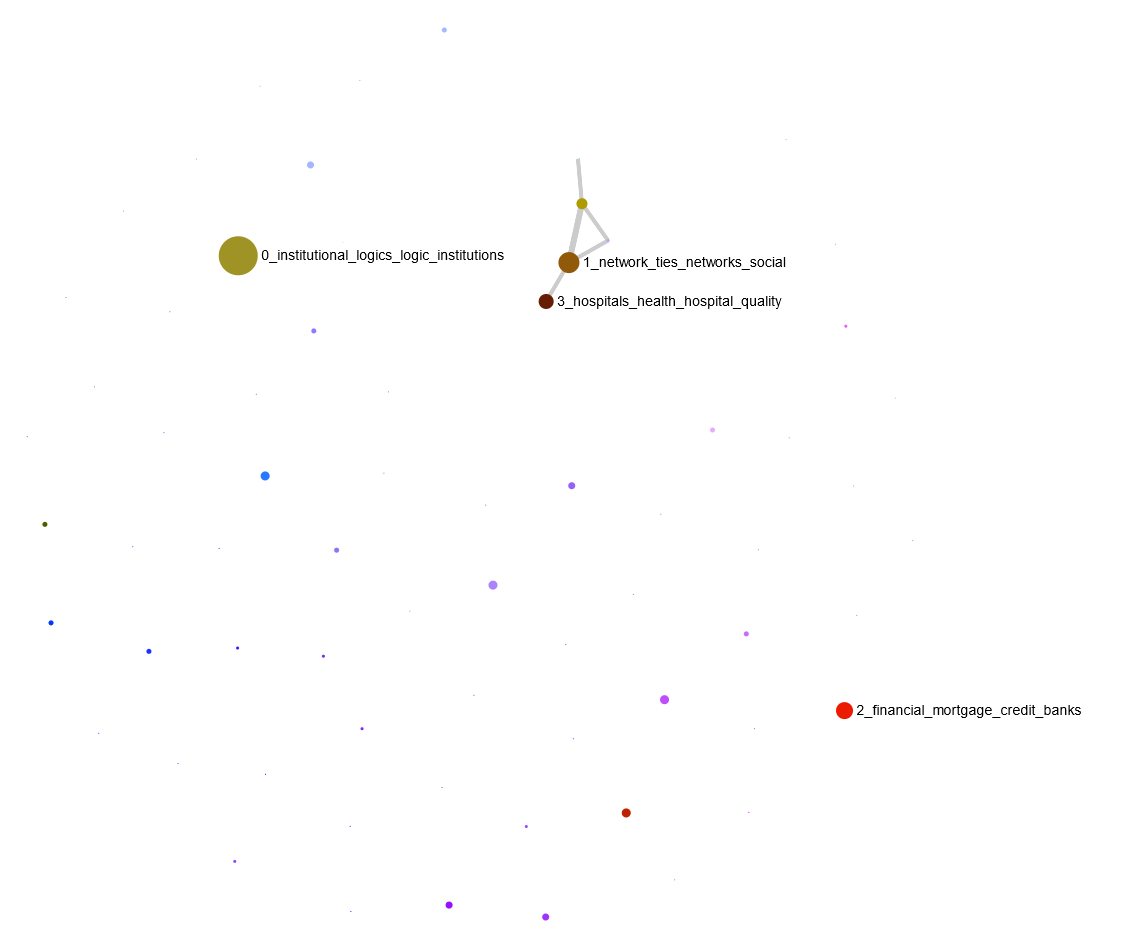
\includegraphics[width=0.7\linewidth]{images/rsog_topic_network_5+.png}
    \caption{EIST Topic Network (Weight 5 or more)}
    \label{fig:enter-label}
\end{figure}






\subsection{Tables}
\subsubsection{Table Columns Explanation} 
\begin{enumerate}
    \item Publication Years: RSOG has the broadest range of publication years (2000-2022), indicating it has been a venue for this research area for a longer time compared to EIST (2011-2022) and SUSSCI (2006-2022).
    Preprocessing Impact: The discrepancy between raw and preprocessed word counts across journals hints at the effectiveness of the pre-processing steps. For example, RSOG's preprocessed word count is much less than its raw count, indicating substantial text cleaning.
    Topic Distribution: The number of topics in each journal is thus expected to provide a preliminary indication of the journal's focus and scope. For instance, despite having fewer articles than SUSSCI, RSOG may have a comparable number of topics, suggesting a shared broader thematic focus.
\end{enumerate}
In summary, our journal-based selection strategy served to demarcate the academic terrain for our CLR with precision, ensuring that the research incorporated was both academically rigorous and directly aligned with our interdisciplinary research objectives. The criteria for article selection in this study were designed to be as inclusive as possible within the bounds of the selected journals, aiming for a comprehensive coverage. We included all full-text articles published in the journals RSOG, EIST, and SUSSCI from their inception to the year 2022. The rationale behind this extensive inclusion criteria is three-fold as enumerated below:
\begin{enumerate}
    \item Temporal Scope: By including articles from the inception of each journal to the present, we were able to capture both foundational works and the most current research in the fields of sociology, environmental innovation, and sustainability science. This allowed for a temporal analysis of trends and shifts in the research landscape, thereby adding a dynamic aspect to our study.
    \item Interdisciplinary Breadth: The selected journals are recognized as leading outlets in intersecting yet distinct disciplines. Including all articles from these journals ensured a rich, interdisciplinary dataset that is aligned with the study's objective to map the interstitial space between sociology, environmental innovation, and societal transitions, and sustainability science.
    \item Volume and Depth for Computational Analysis: The expansive dataset, with a total of 2360 articles comprising over 16 million raw words, provided a sufficiently large corpus for robust computational literature review techniques. The volume of data adds confidence to the machine learning algorithms used for topic modeling and network analysis, as these techniques generally benefit from larger datasets.
\end{enumerate}
Given these aformetntioned reasons, the criteria for article selection were purposefully designed to be broad within the confines of the chosen journals, ensuring a comprehensive and interdisciplinary corpus suitable for advanced computational analysis.
 







\begin{landscape}
\begin{scriptsize} % Reduce font size for the entire table
\begin{longtable}{|>{\scriptsize}c|p{6cm}|c|c|c|c|c|c|c|}
\caption{Temporal Development and Trajectories of Topics Across Three Journals}
\label{tab:my-table-3j_temp_dev} \\ \hline
\textbf{\scriptsize Sr No.} & \textbf{Topic Label} & \textbf{Count} & \textbf{Year Mean} & \textbf{Year Std Dev} & \textbf{Year Min} & \textbf{Year Max} & \textbf{Linear Coeff.} & \textbf{Quadratic Coeff.} \\ \hline
\endfirsthead
%
\multicolumn{9}{c}%
{{\bfseries Table \thetable\ continued from previous page}} \\ \hline
\textbf{\scriptsize Sr No.} & \textbf{Topic Label} & \textbf{Count} & \textbf{Year Mean} & \textbf{Year Std Dev} & \textbf{Year Min} & \textbf{Year Max} & \textbf{Linear Coeff.} & \textbf{Quadratic Coeff.} \\ \hline
\endhead
%
\endfoot
%
\endlastfoot
0 & \textit{0\_interview\_data\_conducted\_participant} & 83 & 2015.154 & 5.447 & 2001 & 2022 & 0.7577 & 0.0673 \\ \hline
1 & \textit{1\_university\_student\_school\_stanford} & 17 & 2015.5 & 3.905 & 2010 & 2021 & -0.877 & 0.1167 \\ \hline
2 & \textit{2\_complexity\_system\_approach\_process} & 52 & 2016.083 & 4.051 & 2009 & 2022 & 0.4452 & 0.0382 \\ \hline
3 & \textit{3\_sustainability\_research\_student\_science} & 36 & 2015.692 & 4.121 & 2009 & 2022 & 0.2857 & 0.0407 \\ \hline
4 & \textit{4\_area\_land\_water\_scenario} & 56 & 2015.077 & 4.731 & 2007 & 2022 & 0.4114 & 0.0731 \\ \hline
5 & \textit{5\_transformation\_actor\_change\_transition} & 48 & 2016.636 & 3.574 & 2011 & 2022 & 0.914 & 0.1026 \\ \hline
6 & \textit{6\_transition\_energy\_policy\_carbon} & 34 & 2016.5 & 3.452 & 2011 & 2022 & 0.4965 & 0.034 \\ \hline
7 & \textit{7\_theory\_organization\_institutional\_volume} & 34 & 2014.846 & 5.475 & 2002 & 2022 & 0.1982 & 0.0137 \\ \hline
8 & \textit{8\_island\_area\_coast\_beach} & 44 & 2013.833 & 4.776 & 2007 & 2022 & 0.1035 & -0.0126 \\ \hline
9 & \textit{9\_emission\_scenario\_reduction\_carbon} & 59 & 2015.667 & 4.661 & 2007 & 2022 & 0.4552 & 0.0298 \\ \hline
10 & \textit{10\_japan\_scenario\_emission\_cost} & 21 & 2016.143 & 4.794 & 2008 & 2022 & 0.2487 & 0.0163 \\ \hline
11 & \textit{11\_diet\_scenario\_food\_consumption} & 18 & 2016.714 & 4.772 & 2008 & 2022 & 0.3082 & 0.0527 \\ \hline
12 & \textit{12\_logic\_institutional\_field\_organization} & 29 & 2016.889 & 3.784 & 2010 & 2022 & -0.2233 & -0.0278 \\ \hline
13 & \textit{13\_biofuels\_fuel\_ethanol\_biofuel} & 19 & 2017.0 & 3.742 & 2011 & 2022 & -0.0317 & -0.0195 \\ \hline
14 & \textit{14\_water\_scenario\_area\_rainfall} & 12 & 2015.875 & 4.781 & 2008 & 2022 & -0.0137 & 0.0073 \\ \hline
15 & \textit{15\_forest\_land\_scenario\_deforestation} & 30 & 2015.583 & 4.172 & 2009 & 2022 & 0.3997 & 0.0608 \\ \hline
16 & \textit{16\_rice\_crop\_yield\_production} & 31 & 2014.933 & 4.434 & 2007 & 2022 & 0.1426 & 0.0185 \\ \hline
17 & \textit{17\_vehicle\_battery\_car\_ev} & 32 & 2016.7 & 4.291 & 2007 & 2022 & 0.2042 & -0.0032 \\ \hline
18 & \textit{18\_religion\_religious\_church\_practice} & 15 & 2017.667 & 3.35 & 2013 & 2022 & -0.0149 & -0.0085 \\ \hline
19 & \textit{19\_synergy\_sdgs\_trade offs\_offs} & 25 & 2017.0 & 4.528 & 2007 & 2022 & 0.3232 & 0.0368 \\ \hline
20 & \textit{20\_transition\_innovation\_technology\_market} & 28 & 2016.5 & 3.452 & 2011 & 2022 & 0.2448 & 0.0085 \\ \hline
21 & \textit{21\_community\_village\_land\_year} & 24 & 2016.167 & 4.017 & 2008 & 2022 & 0.1704 & 0.0122 \\ \hline
22 & \textit{22\_transition\_city\_actor\_process} & 20 & 2019.5 & 1.708 & 2017 & 2022 & 0.2857 & -0.3036 \\ \hline
23 & \textit{23\_paradox\_theory\_logic\_tension} & 29 & 2017.143 & 3.182 & 2011 & 2021 & 0.3508 & 0.3138 \\ \hline
24 & \textit{24\_practice\_object\_logic\_theory} & 26 & 2015.75 & 4.323 & 2009 & 2022 & 0.1906 & 0.072 \\ \hline
25 & \textit{25\_shareholder\_corporation\_firm\_ownership} & 9 & 2018.5 & 2.291 & 2016 & 2022 & 0.8333 & 0.2652 \\ \hline
26 & \textit{26\_hospital\_patient\_nurse\_professional} & 12 & 2012.375 & 7.777 & 2000 & 2021 & 0.0424 & -0.0031 \\ \hline
27 & \textit{27\_variable\_model\_error\_test} & 20 & 2017.0 & 3.367 & 2012 & 2022 & 0.1765 & -0.0398 \\ \hline
28 & \textit{28\_sdgs\_sdg\_target\_indicator} & 8 & 2019.0 & 1.414 & 2017 & 2021 & 0.4 & -0.0 \\ \hline
29 & \textit{29\_system\_approach\_science\_human} & 19 & 2016.667 & 4.955 & 2007 & 2022 & 0.3348 & 0.0502 \\ \hline
30 & \textit{30\_transition\_political\_politics\_policy} & 17 & 2018.667 & 3.249 & 2012 & 2022 & 0.2316 & -0.0307 \\ \hline
31 & \textit{31\_actor\_institution\_process\_theory} & 19 & 2016.667 & 4.0 & 2010 & 2022 & 0.1412 & -0.0367 \\ \hline
32 & \textit{32\_process\_theory\_actor\_action} & 28 & 2016.5 & 4.583 & 2009 & 2022 & 0.2798 & -0.0178 \\ \hline
33 & \textit{33\_disaster\_hazard\_earthquake\_risk} & 13 & 2015.25 & 3.897 & 2010 & 2021 & 0.1214 & 0.0315 \\ \hline
34 & \textit{34\_mortgage\_bank\_loan\_market} & 21 & 2014.667 & 3.682 & 2010 & 2019 & -1.9426 & 0.3278 \\ \hline
35 & \textit{35\_science\_knowledge\_process\_sustainability} & 22 & 2017.222 & 3.521 & 2011 & 2022 & 0.3596 & 0.0343 \\ \hline
36 & \textit{36\_ecological\_scale\_system\_human} & 22 & 2017.889 & 2.767 & 2013 & 2022 & 0.3258 & -0.0262 \\ \hline
37 & \textit{37\_wind\_energy\_power\_solar} & 12 & 2018.143 & 2.231 & 2015 & 2022 & -0.0779 & 0.021 \\ \hline
38 & \textit{38\_crop\_land\_production\_area} & 9 & 2015.333 & 4.784 & 2007 & 2022 & 0.1456 & 0.0291 \\ \hline
39 & \textit{39\_fishery\_fisher\_growth\_ocean} & 8 & 2014.333 & 4.19 & 2010 & 2020 & 0.538 & 0.0714 \\ \hline
40 & \textit{40\_science\_discipline\_sustainability\_university} & 28 & 2016.333 & 4.989 & 2007 & 2022 & 0.1905 & 0.0179 \\ \hline
41 & \textit{41\_interview\_interviewee\_snowball\_sampling} & 10 & 2019.6 & 2.059 & 2016 & 2022 & 0.0 & -0.0 \\ \hline
42 & \textit{42\_process\_system\_technology\_actor} & 12 & 2018.0 & 2.739 & 2014 & 2022 & 0.0833 & 0.0039 \\ \hline
43 & \textit{43\_consumer\_student\_market\_product} & 13 & 2019.167 & 2.115 & 2016 & 2022 & -0.1553 & -0.2333 \\ \hline
44 & \textit{44\_solar\_energy\_grid\_renewable} & 16 & 2018.571 & 2.441 & 2015 & 2022 & 0.5719 & 0.1451 \\ \hline
45 & \textit{45\_church\_religion\_organization\_religious} & 8 & 2018.0 & 2.55 & 2014 & 2021 & -0.6154 & 0.133 \\ \hline
46 & \textit{46\_god\_love\_religion\_world} & 5 & 2014.8 & 4.02 & 2009 & 2021 & 0.0 & -0.0 \\ \hline
47 & \textit{47\_artist\_song\_music\_recording} & 11 & 2014.667 & 4.346 & 2009 & 2021 & 0.1294 & -0.0179 \\ \hline
48 & \textit{48\_bike\_bicycle\_city\_cycling} & 6 & 2019.667 & 1.247 & 2018 & 2021 & 0.2143 & -1.5 \\ \hline
49 & \textit{49\_worker\_white\_whig\_state} & 2 & 2019.0 & 0.0 & 2019 & 2019 &  & 0.0 \\ \hline
50 & \textit{50\_labor\_worker\_union\_platform} & 12 & 2017.667 & 3.197 & 2011 & 2022 & 0.0435 & -0.0075 \\ \hline
51 & \textit{51\_farmer\_sinaloa\_production\_maize} & 11 & 2019.0 & 2.582 & 2014 & 2022 & 0.125 & -0.0356 \\ \hline
52 & \textit{52\_actor\_identity\_institutional\_theory} & 17 & 2017.875 & 3.516 & 2010 & 2022 & 0.1226 & -0.0246 \\ \hline
53 & \textit{53\_paris\_agreement\_emission\_climate} & 6 & 2020.5 & 1.118 & 2019 & 2022 & -0.4 & -0.0 \\ \hline
54 & \textit{54\_transition\_innovation\_framework\_literature} & 9 & 2020.0 & 1.414 & 2018 & 2022 & 0.6 & 0.1429 \\ \hline
55 & \textit{55\_logic\_organization\_identity\_process} & 10 & 2015.125 & 6.698 & 2001 & 2022 & -0.0091 & -0.0049 \\ \hline
56 & \textit{56\_ecological\_social\_human\_change} & 20 & 2015.9 & 4.614 & 2008 & 2022 & 0.108 & 0.0449 \\ \hline
57 & \textit{57\_stakeholder\_project\_process\_level} & 10 & 2017.0 & 3.464 & 2012 & 2022 & 0.1042 & 0.0342 \\ \hline
58 & \textit{58\_capitalist\_world\_colonialism\_colonial} & 9 & 2018.5 & 3.5 & 2015 & 2022 & 1.0 & 0.0002 \\ \hline
59 & \textit{59\_qca\_condition\_configuration\_case} & 4 & 2017.0 & 4.0 & 2013 & 2021 & -0.25 & -0.0001 \\ \hline
60 & \textit{60\_forest\_farmer\_land\_landscape} & 9 & 2017.2 & 5.269 & 2007 & 2022 & 0.0014 & 0.0229 \\ \hline
61 & \textit{61\_cost\_technology\_electricity\_energy} & 9 & 2016.0 & 4.213 & 2007 & 2021 & 0.0352 & 0.0087 \\ \hline
62 & \textit{62\_configuration\_qca\_outcome\_case} & 8 & 2015.0 & 2.0 & 2013 & 2017 & -1.5 & -0.0004 \\ \hline
63 & \textit{63\_entrepreneur\_organizational\_entrepreneurship\_institutional} & 5 & 2016.0 & 4.195 & 2009 & 2021 & 0.0 & -0.0 \\ \hline
64 & \textit{64\_category\_audience\_analyst\_identity} & 19 & 2016.286 & 4.463 & 2009 & 2021 & 0.126 & -0.0548 \\ \hline
65 & \textit{65\_stanford\_school\_student\_university} & 15 & 2014.5 & 4.5 & 2010 & 2019 & -1.4444 & -0.0004 \\ \hline
66 & \textit{66\_change\_climate\_ecological\_ecosystem} & 14 & 2015.083 & 4.387 & 2007 & 2022 & 0.0383 & 0.0055 \\ \hline
67 & \textit{67\_organization\_theory\_process\_structure} & 9 & 2017.375 & 4.091 & 2009 & 2022 & 0.0121 & -0.0043 \\ \hline
68 & \textit{68\_island\_atoll\_area\_coast} & 6 & 2015.667 & 3.091 & 2013 & 2020 & -0.2791 & 0.4286 \\ \hline
69 & \textit{69\_multimodal\_visual\_mode\_multimodality} & 13 & 2018.4 & 3.2 & 2013 & 2022 & -0.2188 & -0.2392 \\ \hline
70 & \textit{70\_farmer\_food\_crop\_farming} & 20 & 2013.7 & 4.383 & 2007 & 2022 & 0.2082 & 0.0411 \\ \hline
71 & \textit{71\_city\_urban\_experiment\_myth} & 6 & 2017.5 & 1.803 & 2015 & 2020 & 0.2308 & -0.0 \\ \hline
72 & \textit{72\_synergy\_target\_sdgs\_trade offs} & 7 & 2021.0 & 1.0 & 2020 & 2022 & 0.5 & 0.0001 \\ \hline
73 & \textit{73\_group\_community\_resource\_change} & 21 & 2015.818 & 5.06 & 2006 & 2022 & 0.152 & 0.0241 \\ \hline
74 & \textit{74\_behavior\_decision\_theory\_psychological} & 17 & 2017.0 & 3.801 & 2010 & 2022 & 0.1308 & -0.0061 \\ \hline
75 & \textit{75\_researcher\_university\_research\_academic} & 13 & 2016.625 & 2.497 & 2013 & 2021 & 0.0376 & 0.0214 \\ \hline
76 & \textit{76\_interview\_data\_coding\_analysis} & 10 & 2019.2 & 2.315 & 2016 & 2022 & 0.2612 & 0.1268 \\ \hline
77 & \textit{77\_race\_racial\_discrimination\_inequality} & 10 & 2013.75 & 6.869 & 2002 & 2019 & 0.151 & 0.0669 \\ \hline
78 & \textit{78\_food\_transition\_agri food\_agri} & 6 & 2019.75 & 2.278 & 2016 & 2022 & 0.0723 & -0.1358 \\ \hline
79 & \textit{79\_sustainability\_change\_transition\_environmental} & 12 & 2015.125 & 5.395 & 2007 & 2022 & 0.1052 & 0.017 \\ \hline
80 & \textit{80\_mortgage\_meltdown\_crisis\_loan} & 10 & 2010.0 & 0.0 & 2010 & 2010 &  & 0.0 \\ \hline
81 & \textit{81\_nature\_biodiversity\_ecosystem\_human} & 9 & 2019.5 & 2.291 & 2016 & 2022 & 0.1667 & -0.1591 \\ \hline
82 & \textit{82\_practice\_logic\_meaning\_action} & 10 & 2017.333 & 4.534 & 2009 & 2022 & 0.0378 & 0.0405 \\ \hline
83 & \textit{83\_disease\_farm\_pathogen\_farmer} & 7 & 2019.75 & 2.278 & 2016 & 2022 & 0.1325 & -0.1186 \\ \hline
84 & \textit{84\_case\_theory\_research\_transferability} & 16 & 2018.143 & 3.681 & 2010 & 2022 & 0.2711 & 0.0663 \\ \hline
85 & \textit{85\_bioeconomy\_bio\_biorefineries\_zealand} & 10 & 2016.857 & 3.681 & 2011 & 2022 & 0.1416 & 0.0397 \\ \hline
86 & \textit{86\_transition\_policy\_technology\_innovation} & 10 & 2016.0 & 5.043 & 2007 & 2022 & 0.0449 & -0.0074 \\ \hline
87 & \textit{87\_interview\_snowball\_sampling\_interviewee} & 10 & 2015.889 & 5.858 & 2002 & 2022 & 0.0133 & 0.0011 \\ \hline
88 & \textit{88\_energy\_nuclear\_coalition\_electricity} & 16 & 2017.125 & 2.976 & 2011 & 2021 & 0.0847 & -0.0315 \\ \hline
89 & \textit{89\_car\_vehicle\_transport\_sharing} & 7 & 2018.4 & 2.154 & 2015 & 2021 & 0.0086 & -0.0709 \\ \hline
90 & \textit{90\_landscape\_ecosystem\_biodiversity\_tree} & 10 & 2018.2 & 2.561 & 2015 & 2022 & 0.3354 & -0.091 \\ \hline
91 & \textit{91\_process\_actor\_conflict\_knowledge} & 6 & 2017.2 & 4.707 & 2011 & 2022 & 0.0433 & 0.0411 \\ \hline
92 & \textit{92\_science\_research\_sustainability\_problem} & 10 & 2017.75 & 3.269 & 2012 & 2022 & -0.0292 & 0.0277 \\ \hline
93 & \textit{93\_water\_management\_basin\_decision} & 16 & 2018.0 & 2.582 & 2014 & 2022 & 0.0833 & -0.0119 \\ \hline
94 & \textit{94\_meaning\_actor\_discourse\_form} & 16 & 2017.625 & 3.389 & 2011 & 2022 & 0.0327 & 0.0454 \\ \hline
95 & \textit{95\_africa\_african\_barometer\_malawi} & 7 & 2016.6 & 3.611 & 2011 & 2022 & 0.0123 & -0.0258 \\ \hline
96 & \textit{96\_water\_resource\_country\_year} & 10 & 2015.222 & 5.245 & 2007 & 2022 & -0.0332 & 0.0097 \\ \hline
97 & \textit{97\_transformation\_sustainability\_transition\_change} & 10 & 2016.5 & 4.717 & 2009 & 2022 & 0.2584 & 0.0382 \\ \hline
98 & \textit{98\_process\_system\_place\_knowledge} & 10 & 2018.4 & 2.728 & 2015 & 2022 & -0.1613 & 0.0655 \\ \hline
99 & \textit{99\_marine\_tourism\_island\_rc} & 13 & 2018.5 & 2.986 & 2014 & 2022 & 0.215 & 0.0599 \\ \hline
100 & \textit{100\_process\_system\_innovation\_actor} & 11 & 2014.857 & 6.999 & 2001 & 2022 & 0.0687 & 0.007 \\ \hline
101 & \textit{101\_island\_port\_adaptation\_atoll} & 5 & 2013.4 & 4.587 & 2008 & 2020 & 0.0 & -0.0 \\ \hline
102 & \textit{102\_tree\_forest\_landscape\_deforestation} & 4 & 2019.5 & 1.803 & 2017 & 2022 & 0.0 & -0.0 \\ \hline
103 & \textit{103\_bias\_sample\_survey\_respondent} & 12 & 2018.833 & 2.672 & 2014 & 2022 & 0.2101 & -0.0335 \\ \hline
104 & \textit{104\_technology\_industry\_module\_solar} & 10 & 2018.167 & 2.911 & 2014 & 2022 & -0.0328 & -0.0967 \\ \hline
105 & \textit{105\_farm\_farmer\_land\_crop} & 9 & 2018.0 & 2.739 & 2014 & 2022 & -0.0167 & -0.0252 \\ \hline
106 & \textit{106\_nature\_value\_concept\_relational} & 10 & 2019.8 & 1.72 & 2017 & 2022 & 0.0 & 0.109 \\ \hline
107 & \textit{107\_fishery\_fisher\_bay\_co management} & 3 & 2015.0 & 4.899 & 2009 & 2021 & 0.0 & 0.0 \\ \hline
108 & \textit{108\_company\_cost\_grid\_industry} & 9 & 2019.0 & 2.0 & 2016 & 2022 & 0.05 & 0.0357 \\ \hline
109 & \textit{109\_carbon\_emission\_low\_technology} & 9 & 2016.286 & 4.061 & 2011 & 2022 & 0.0903 & 0.0211 \\ \hline
110 & \textit{110\_airline\_aircraft\_atp\_shipowner} & 3 & 2016.0 & 2.449 & 2013 & 2019 & 0.0 & 0.0 \\ \hline
111 & \textit{111\_city\_urban\_community\_transition} & 9 & 2017.0 & 3.571 & 2012 & 2022 & 0.0098 & -0.0188 \\ \hline
112 & \textit{112\_actor\_role\_perspective\_process} & 8 & 2019.0 & 2.38 & 2015 & 2022 & 0.0588 & -0.0375 \\ \hline
113 & \textit{113\_community\_system\_approach\_management} & 12 & 2019.167 & 2.115 & 2016 & 2022 & 0.3727 & 0.319 \\ \hline
114 & \textit{114\_transition\_innovation\_energy\_policy} & 25 & 2017.2 & 3.25 & 2012 & 2022 & 0.4072 & 0.0274 \\ \hline
115 & \textit{115\_problem\_future\_solution\_sustainability} & 12 & 2016.889 & 4.012 & 2010 & 2022 & 0.1058 & 0.0428 \\ \hline
116 & \textit{116\_impact\_design\_case\_output} & 6 & 2017.0 & 2.28 & 2014 & 2020 & -0.1154 & 0.0646 \\ \hline
117 & \textit{117\_japan\_capital\_prefecture\_iwi} & 6 & 2019.5 & 1.708 & 2017 & 2022 & 0.0 & -0.0 \\ \hline
118 & \textit{118\_dialogue\_discourse\_actor\_debate} & 10 & 2018.5 & 2.986 & 2013 & 2022 & 0.0748 & 0.0797 \\ \hline
119 & \textit{119\_storm\_cyclone\_sheet\_wind} & 9 & 2014.857 & 4.611 & 2008 & 2022 & -0.0115 & -0.0149 \\ \hline
120 & \textit{120\_external\_firm\_externality\_company} & 11 & 2015.571 & 5.473 & 2007 & 2022 & -0.0157 & -0.0145 \\ \hline
121 & \textit{121\_firm\_clique\_membership\_member} & 8 & 2011.0 & 5.477 & 2001 & 2017 & 0.0133 & 0.0293 \\ \hline
122 & \textit{122\_organization\_external\_firm\_resource} & 10 & 2012.571 & 5.925 & 2001 & 2019 & -0.007 & 0.0092 \\ \hline
123 & \textit{123\_vulnerability\_climate\_change\_exposure} & 10 & 2015.0 & 5.158 & 2007 & 2022 & 0.0 & -0.0 \\ \hline
124 & \textit{124\_process\_context\_change\_niche} & 20 & 2018.833 & 2.544 & 2015 & 2022 & 0.3433 & -0.0442 \\ \hline
125 & \textit{125\_actor\_routine\_action\_acceleration} & 9 & 2018.167 & 3.436 & 2013 & 2022 & 0.1059 & -0.0033 \\ \hline
126 & \textit{126\_organization\_individual\_form\_action} & 13 & 2013.0 & 6.797 & 2000 & 2021 & 0.026 & -0.0001 \\ \hline
127 & \textit{127\_crop\_area\_forest\_land} & 11 & 2016.75 & 4.235 & 2010 & 2022 & 0.0958 & 0.024 \\ \hline
128 & \textit{128\_delta\_sediment\_basin\_area} & 9 & 2015.5 & 4.61 & 2009 & 2022 & 0.0294 & -0.0595 \\ \hline
129 & \textit{129\_system\_market\_technology\_transition} & 7 & 2020.5 & 1.118 & 2019 & 2022 & 0.1 & -0.75 \\ \hline
130 & \textit{130\_technology\_transition\_country\_market} & 13 & 2018.125 & 2.848 & 2013 & 2022 & 0.1599 & 0.0003 \\ \hline
131 & \textit{131\_waste\_material\_recycling\_landfill} & 7 & 2013.167 & 4.879 & 2007 & 2022 & 0.0618 & 0.0087 \\ \hline
132 & \textit{132\_transition\_system\_market\_technology} & 10 & 2017.833 & 4.67 & 2008 & 2022 & 0.0586 & -0.0068 \\ \hline
133 & \textit{133\_actor\_organization\_logic\_field} & 9 & 2018.0 & 2.16 & 2015 & 2021 & 0.2143 & 0.0 \\ \hline
134 & \textit{134\_city\_urban\_environment\_ri city} & 9 & 2018.0 & 3.958 & 2010 & 2022 & 0.0319 & -0.0215 \\ \hline
135 & \textit{135\_variable\_model\_score\_regression} & 9 & 2015.0 & 6.608 & 2001 & 2021 & 0.0153 & -0.0131 \\ \hline
136 & \textit{136\_woman\_child\_family\_migration} & 3 & 2015.5 & 6.5 & 2009 & 2022 & 0.0769 & 0.0 \\ \hline
137 & \textit{137\_game\_approach\_process\_change} & 22 & 2015.6 & 4.944 & 2007 & 2022 & 0.2447 & 0.0356 \\ \hline
\end{longtable}
\end{scriptsize} % End the reduced font size
\end{landscape}



% Please add the following required packages to your document preamble:
% \usepackage{lscape}
% \usepackage{longtable}
% Note: It may be necessary to compile the document several times to get a multi-page table to line up properly
%\begin{landscape}
\begin{longtable}{|l|l|l|l|l|}
\caption{Descriptive Statistics of the Three Journal Topic Landscape}
\label{tab:my-table-dscrstat}\\
\hline
\textbf{} & \textbf{Topic Label} & \textbf{standardized\_mean} & \textbf{max} & \textbf{min} \\ \hline
\endfirsthead
%
\multicolumn{5}{c}%
{{\bfseries Table \thetable\ continued from previous page}} \\
\hline
\textbf{} & \textbf{Topic Label} & \textbf{standardized\_mean} & \textbf{max} & \textbf{min} \\ \hline
\endhead
%
0 & \textit{0\_interview\_data\_conducted\_participant} & 3.637 & 0.56 & 0.0 \\ \hline
1 & \textit{1\_university\_student\_school\_stanford} & 1.789 & 0.951 & 0.0 \\ \hline
2 & \textit{2\_complexity\_system\_approach\_process} & 1.542 & 0.63 & 0.0 \\ \hline
3 & \textit{3\_sustainability\_research\_student\_science} & 1.447 & 0.863 & 0.0 \\ \hline
4 & \textit{4\_area\_land\_water\_scenario} & 3.686 & 0.854 & 0.0 \\ \hline
5 & \textit{5\_transformation\_actor\_change\_transition} & 1.559 & 0.83 & 0.0 \\ \hline
6 & \textit{6\_transition\_energy\_policy\_carbon} & 1.273 & 0.896 & 0.0 \\ \hline
7 & \textit{7\_theory\_organization\_institutional\_volume} & 1.189 & 0.476 & 0.0 \\ \hline
8 & \textit{8\_island\_area\_coast\_beach} & 4.017 & 0.924 & 0.0 \\ \hline
9 & \textit{9\_emission\_scenario\_reduction\_carbon} & 2.888 & 0.602 & 0.0 \\ \hline
10 & \textit{10\_japan\_scenario\_emission\_cost} & 1.927 & 0.825 & 0.0 \\ \hline
11 & \textit{11\_diet\_scenario\_food\_consumption} & 1.392 & 0.766 & 0.0 \\ \hline
12 & \textit{12\_logic\_institutional\_field\_organization} & 1.716 & 0.854 & 0.0 \\ \hline
13 & \textit{13\_biofuels\_fuel\_ethanol\_biofuel} & 1.413 & 0.833 & 0.0 \\ \hline
14 & \textit{14\_water\_scenario\_area\_rainfall} & 0.695 & 0.576 & 0.0 \\ \hline
15 & \textit{15\_forest\_land\_scenario\_deforestation} & 1.513 & 0.526 & 0.0 \\ \hline
16 & \textit{16\_rice\_crop\_yield\_production} & 1.652 & 0.85 & 0.0 \\ \hline
17 & \textit{17\_vehicle\_battery\_car\_ev} & 3.389 & 0.877 & 0.0 \\ \hline
18 & \textit{18\_religion\_religious\_church\_practice} & 0.744 & 0.743 & 0.0 \\ \hline
19 & \textit{19\_synergy\_sdgs\_trade offs\_offs} & 0.893 & 0.755 & 0.0 \\ \hline
20 & \textit{20\_transition\_innovation\_technology\_market} & 1.361 & 0.833 & 0.0 \\ \hline
21 & \textit{21\_community\_village\_land\_year} & 1.14 & 0.742 & 0.0 \\ \hline
22 & \textit{22\_transition\_city\_actor\_process} & 1.085 & 0.527 & 0.0 \\ \hline
23 & \textit{23\_paradox\_theory\_logic\_tension} & 1.777 & 0.727 & 0.0 \\ \hline
24 & \textit{24\_practice\_object\_logic\_theory} & 1.21 & 0.737 & 0.0 \\ \hline
25 & \textit{25\_shareholder\_corporation\_firm\_ownership} & 0.718 & 0.706 & 0.0 \\ \hline
26 & \textit{26\_hospital\_patient\_nurse\_professional} & 1.406 & 0.831 & 0.0 \\ \hline
27 & \textit{27\_variable\_model\_error\_test} & 0.837 & 0.477 & 0.0 \\ \hline
28 & \textit{28\_sdgs\_sdg\_target\_indicator} & 0.684 & 0.641 & 0.0 \\ \hline
29 & \textit{29\_system\_approach\_science\_human} & 1.003 & 0.417 & 0.0 \\ \hline
30 & \textit{30\_transition\_political\_politics\_policy} & 0.908 & 0.697 & 0.0 \\ \hline
31 & \textit{31\_actor\_institution\_process\_theory} & 0.959 & 0.542 & 0.0 \\ \hline
32 & \textit{32\_process\_theory\_actor\_action} & 1.125 & 0.449 & 0.0 \\ \hline
33 & \textit{33\_disaster\_hazard\_earthquake\_risk} & 0.723 & 0.51 & 0.0 \\ \hline
34 & \textit{34\_mortgage\_bank\_loan\_market} & 1.833 & 0.793 & 0.0 \\ \hline
35 & \textit{35\_science\_knowledge\_process\_sustainability} & 1.129 & 0.563 & 0.0 \\ \hline
36 & \textit{36\_ecological\_scale\_system\_human} & 1.1 & 0.62 & 0.0 \\ \hline
37 & \textit{37\_wind\_energy\_power\_solar} & 0.604 & 0.35 & 0.0 \\ \hline
38 & \textit{38\_crop\_land\_production\_area} & 0.663 & 0.424 & 0.0 \\ \hline
39 & \textit{39\_fishery\_fisher\_growth\_ocean} & 1.302 & 0.832 & 0.0 \\ \hline
40 & \textit{40\_science\_discipline\_sustainability\_university} & 1.205 & 1.0 & 0.0 \\ \hline
41 & \textit{41\_interview\_interviewee\_snowball\_sampling} & 0.577 & 0.462 & 0.0 \\ \hline
42 & \textit{42\_process\_system\_technology\_actor} & 0.916 & 0.38 & 0.0 \\ \hline
43 & \textit{43\_consumer\_student\_market\_product} & 0.787 & 0.799 & 0.0 \\ \hline
44 & \textit{44\_solar\_energy\_grid\_renewable} & 0.775 & 0.637 & 0.0 \\ \hline
45 & \textit{45\_church\_religion\_organization\_religious} & 0.639 & 0.622 & 0.0 \\ \hline
46 & \textit{46\_god\_love\_religion\_world} & 0.618 & 0.695 & 0.0 \\ \hline
47 & \textit{47\_artist\_song\_music\_recording} & 1.363 & 0.85 & 0.0 \\ \hline
48 & \textit{48\_bike\_bicycle\_city\_cycling} & 1.151 & 0.847 & 0.0 \\ \hline
49 & \textit{49\_worker\_white\_whig\_state} & 0.605 & 0.9 & 0.0 \\ \hline
50 & \textit{50\_labor\_worker\_union\_platform} & 0.964 & 0.73 & 0.0 \\ \hline
51 & \textit{51\_farmer\_sinaloa\_production\_maize} & 0.81 & 1.0 & 0.0 \\ \hline
52 & \textit{52\_actor\_identity\_institutional\_theory} & 0.885 & 0.686 & 0.0 \\ \hline
53 & \textit{53\_paris\_agreement\_emission\_climate} & 0.599 & 0.484 & 0.0 \\ \hline
54 & \textit{54\_transition\_innovation\_framework\_literature} & 0.7 & 0.451 & 0.0 \\ \hline
55 & \textit{55\_logic\_organization\_identity\_process} & 0.92 & 0.439 & 0.0 \\ \hline
56 & \textit{56\_ecological\_social\_human\_change} & 0.953 & 0.851 & 0.0 \\ \hline
57 & \textit{57\_stakeholder\_project\_process\_level} & 1.025 & 0.652 & 0.0 \\ \hline
58 & \textit{58\_capitalist\_world\_colonialism\_colonial} & 0.826 & 0.669 & 0.0 \\ \hline
59 & \textit{59\_qca\_condition\_configuration\_case} & 0.599 & 0.473 & 0.0 \\ \hline
60 & \textit{60\_forest\_farmer\_land\_landscape} & 0.789 & 0.394 & 0.0 \\ \hline
61 & \textit{61\_cost\_technology\_electricity\_energy} & 0.731 & 0.493 & 0.0 \\ \hline
62 & \textit{62\_configuration\_qca\_outcome\_case} & 0.77 & 0.513 & 0.0 \\ \hline
63 & \textit{63\_entrepreneur\_organizational\_entrepreneurship\_institutional} & 0.627 & 0.662 & 0.0 \\ \hline
64 & \textit{64\_category\_audience\_analyst\_identity} & 1.137 & 0.549 & 0.0 \\ \hline
65 & \textit{65\_stanford\_school\_student\_university} & 0.768 & 0.851 & 0.0 \\ \hline
66 & \textit{66\_change\_climate\_ecological\_ecosystem} & 0.829 & 0.584 & 0.0 \\ \hline
67 & \textit{67\_organization\_theory\_process\_structure} & 0.707 & 0.567 & 0.0 \\ \hline
68 & \textit{68\_island\_atoll\_area\_coast} & 0.561 & 0.431 & 0.0 \\ \hline
69 & \textit{69\_multimodal\_visual\_mode\_multimodality} & 1.298 & 0.687 & 0.0 \\ \hline
70 & \textit{70\_farmer\_food\_crop\_farming} & 0.98 & 0.582 & 0.0 \\ \hline
71 & \textit{71\_city\_urban\_experiment\_myth} & 0.67 & 0.66 & 0.0 \\ \hline
72 & \textit{72\_synergy\_target\_sdgs\_trade offs} & 0.593 & 0.399 & 0.0 \\ \hline
73 & \textit{73\_group\_community\_resource\_change} & 1.182 & 0.751 & 0.0 \\ \hline
74 & \textit{74\_behavior\_decision\_theory\_psychological} & 0.995 & 0.652 & 0.0 \\ \hline
75 & \textit{75\_researcher\_university\_research\_academic} & 0.875 & 0.661 & 0.0 \\ \hline
76 & \textit{76\_interview\_data\_coding\_analysis} & 0.736 & 0.387 & 0.0 \\ \hline
77 & \textit{77\_race\_racial\_discrimination\_inequality} & 0.731 & 0.905 & 0.0 \\ \hline
78 & \textit{78\_food\_transition\_agri food\_agri} & 0.665 & 0.979 & 0.0 \\ \hline
79 & \textit{79\_sustainability\_change\_transition\_environmental} & 0.799 & 0.692 & 0.0 \\ \hline
80 & \textit{80\_mortgage\_meltdown\_crisis\_loan} & 0.572 & 0.387 & 0.0 \\ \hline
81 & \textit{81\_nature\_biodiversity\_ecosystem\_human} & 0.77 & 0.734 & 0.0 \\ \hline
82 & \textit{82\_practice\_logic\_meaning\_action} & 0.88 & 0.409 & 0.0 \\ \hline
83 & \textit{83\_disease\_farm\_pathogen\_farmer} & 0.655 & 0.484 & 0.0 \\ \hline
84 & \textit{84\_case\_theory\_research\_transferability} & 0.886 & 0.563 & 0.0 \\ \hline
85 & \textit{85\_bioeconomy\_bio\_biorefineries\_zealand} & 0.715 & 1.0 & 0.0 \\ \hline
86 & \textit{86\_transition\_policy\_technology\_innovation} & 0.751 & 0.504 & 0.0 \\ \hline
87 & \textit{87\_interview\_snowball\_sampling\_interviewee} & 0.571 & 0.533 & 0.0 \\ \hline
88 & \textit{88\_energy\_nuclear\_coalition\_electricity} & 0.89 & 0.414 & 0.0 \\ \hline
89 & \textit{89\_car\_vehicle\_transport\_sharing} & 0.619 & 0.932 & 0.0 \\ \hline
90 & \textit{90\_landscape\_ecosystem\_biodiversity\_tree} & 0.801 & 0.484 & 0.0 \\ \hline
91 & \textit{91\_process\_actor\_conflict\_knowledge} & 0.773 & 0.77 & 0.0 \\ \hline
92 & \textit{92\_science\_research\_sustainability\_problem} & 0.84 & 0.493 & 0.0 \\ \hline
93 & \textit{93\_water\_management\_basin\_decision} & 0.995 & 1.0 & 0.0 \\ \hline
94 & \textit{94\_meaning\_actor\_discourse\_form} & 0.855 & 0.474 & 0.0 \\ \hline
95 & \textit{95\_africa\_african\_barometer\_malawi} & 0.699 & 0.844 & 0.0 \\ \hline
96 & \textit{96\_water\_resource\_country\_year} & 0.811 & 0.665 & 0.0 \\ \hline
97 & \textit{97\_transformation\_sustainability\_transition\_change} & 0.733 & 0.47 & 0.0 \\ \hline
98 & \textit{98\_process\_system\_place\_knowledge} & 0.851 & 0.405 & 0.0 \\ \hline
99 & \textit{99\_marine\_tourism\_island\_rc} & 0.842 & 0.69 & 0.0 \\ \hline
100 & \textit{100\_process\_system\_innovation\_actor} & 0.823 & 0.389 & 0.0 \\ \hline
101 & \textit{101\_island\_port\_adaptation\_atoll} & 0.598 & 0.7 & 0.0 \\ \hline
102 & \textit{102\_tree\_forest\_landscape\_deforestation} & 0.612 & 0.774 & 0.0 \\ \hline
103 & \textit{103\_bias\_sample\_survey\_respondent} & 0.699 & 0.387 & 0.0 \\ \hline
104 & \textit{104\_technology\_industry\_module\_solar} & 0.732 & 0.624 & 0.0 \\ \hline
105 & \textit{105\_farm\_farmer\_land\_crop} & 0.736 & 0.649 & 0.0 \\ \hline
106 & \textit{106\_nature\_value\_concept\_relational} & 0.763 & 0.646 & 0.0 \\ \hline
107 & \textit{107\_fishery\_fisher\_bay\_co management} & 0.546 & 0.847 & 0.0 \\ \hline
108 & \textit{108\_company\_cost\_grid\_industry} & 0.81 & 0.385 & 0.0 \\ \hline
109 & \textit{109\_carbon\_emission\_low\_technology} & 0.716 & 0.529 & 0.0 \\ \hline
110 & \textit{110\_airline\_aircraft\_atp\_shipowner} & 0.463 & 0.778 & 0.0 \\ \hline
111 & \textit{111\_city\_urban\_community\_transition} & 0.818 & 0.626 & 0.0 \\ \hline
112 & \textit{112\_actor\_role\_perspective\_process} & 0.749 & 0.48 & 0.0 \\ \hline
113 & \textit{113\_community\_system\_approach\_management} & 0.91 & 0.427 & 0.0 \\ \hline
114 & \textit{114\_transition\_innovation\_energy\_policy} & 1.008 & 0.95 & 0.0 \\ \hline
115 & \textit{115\_problem\_future\_solution\_sustainability} & 0.769 & 0.373 & 0.0 \\ \hline
116 & \textit{116\_impact\_design\_case\_output} & 0.682 & 0.445 & 0.0 \\ \hline
117 & \textit{117\_japan\_capital\_prefecture\_iwi} & 0.613 & 0.67 & 0.0 \\ \hline
118 & \textit{118\_dialogue\_discourse\_actor\_debate} & 0.782 & 0.495 & 0.0 \\ \hline
119 & \textit{119\_storm\_cyclone\_sheet\_wind} & 0.686 & 0.789 & 0.0 \\ \hline
120 & \textit{120\_external\_firm\_externality\_company} & 0.776 & 0.538 & 0.0 \\ \hline
121 & \textit{121\_firm\_clique\_membership\_member} & 0.762 & 0.496 & 0.0 \\ \hline
122 & \textit{122\_organization\_external\_firm\_resource} & 0.841 & 0.716 & 0.0 \\ \hline
123 & \textit{123\_vulnerability\_climate\_change\_exposure} & 0.701 & 0.443 & 0.0 \\ \hline
124 & \textit{124\_process\_context\_change\_niche} & 1.066 & 0.551 & 0.0 \\ \hline
125 & \textit{125\_actor\_routine\_action\_acceleration} & 0.729 & 0.332 & 0.0 \\ \hline
126 & \textit{126\_organization\_individual\_form\_action} & 1.019 & 0.566 & 0.0 \\ \hline
127 & \textit{127\_crop\_area\_forest\_land} & 0.785 & 0.469 & 0.0 \\ \hline
128 & \textit{128\_delta\_sediment\_basin\_area} & 0.79 & 0.669 & 0.0 \\ \hline
129 & \textit{129\_system\_market\_technology\_transition} & 0.841 & 0.599 & 0.0 \\ \hline
130 & \textit{130\_technology\_transition\_country\_market} & 0.875 & 0.472 & 0.0 \\ \hline
131 & \textit{131\_waste\_material\_recycling\_landfill} & 0.698 & 0.722 & 0.0 \\ \hline
132 & \textit{132\_transition\_system\_market\_technology} & 0.949 & 0.663 & 0.0 \\ \hline
133 & \textit{133\_actor\_organization\_logic\_field} & 0.688 & 0.447 & 0.0 \\ \hline
134 & \textit{134\_city\_urban\_environment\_ri city} & 0.73 & 0.702 & 0.0 \\ \hline
135 & \textit{135\_variable\_model\_score\_regression} & 0.708 & 0.648 & 0.0 \\ \hline
136 & \textit{136\_woman\_child\_family\_migration} & 0.614 & 0.718 & 0.0 \\ \hline
137 & \textit{137\_game\_approach\_process\_change} & 1.12 & 0.446 & 0.0 \\ \hline
\end{longtable}


%\end{landscape}

\onecolumn
% Please add the following required packages to your document preamble:
% \usepackage{lscape}
% \usepackage{longtable}
% Note: It may be necessary to compile the document several times to get a multi-page table to line up properly
%\begin{landscape}
\begin{longtable}{|l|l|l|l|l|}
\caption{Descriptive Statistics EIST}
\label{tab:my-table-dseist}\\
\hline
\textbf{} & \textit{\textbf{Topic Label}} & \textbf{standardized\_mean} & \textbf{max} & \textbf{min} \\ \hline
\endfirsthead
%
\multicolumn{5}{c}%
{{\bfseries Table \thetable\ continued from previous page}} \\
\hline
\textbf{} & \textit{\textbf{Topic Label}} & \textbf{standardized\_mean} & \textbf{max} & \textbf{min} \\ \hline
\endhead
%
0 & \textit{0\_interview\_data\_conducted\_structured} & 1.365 & 0.576 & 0.0 \\ \hline
1 & \textit{1\_biofuels\_fuel\_bioeconomy\_market} & 1.333 & 0.818 & 0.0 \\ \hline
2 & \textit{2\_transition\_research\_sustainability\_political} & 1.921 & 0.865 & 0.0 \\ \hline
3 & \textit{3\_actor\_transition\_change\_process} & 1.645 & 0.744 & 0.0 \\ \hline
4 & \textit{4\_farmer\_farming\_farm\_food} & 1.305 & 0.841 & 0.0 \\ \hline
5 & \textit{5\_transition\_study\_framework\_research} & 0.839 & 0.448 & 0.0 \\ \hline
6 & \textit{6\_case\_study\_analysis\_research} & 1.019 & 0.74 & 0.0 \\ \hline
7 & \textit{7\_service\_time\_project\_economy} & 1.882 & 0.937 & 0.0 \\ \hline
8 & \textit{8\_car\_vehicle\_battery\_sharing} & 1.528 & 0.953 & 0.0 \\ \hline
9 & \textit{9\_coal\_energy\_technology\_policy} & 1.014 & 0.776 & 0.0 \\ \hline
10 & \textit{10\_solar\_energy\_grid\_industry} & 0.839 & 0.584 & 0.0 \\ \hline
11 & \textit{11\_bike\_city\_bicycle\_cycling} & 1.299 & 0.924 & 0.0 \\ \hline
12 & \textit{12\_innovation\_actor\_change\_field} & 1.099 & 0.479 & 0.0 \\ \hline
13 & \textit{13\_building\_construction\_project\_intermediary} & 0.912 & 0.852 & 0.0 \\ \hline
14 & \textit{14\_complexity\_transition\_process\_system} & 0.826 & 0.455 & 0.0 \\ \hline
15 & \textit{15\_transition\_practice\_process\_system} & 0.807 & 0.772 & 0.0 \\ \hline
16 & \textit{16\_food\_system\_transition\_agri food} & 1.097 & 1.0 & 0.0 \\ \hline
17 & \textit{17\_car\_manufacturer\_vehicle\_automobile} & 0.856 & 0.832 & 0.0 \\ \hline
18 & \textit{18\_transition\_energy\_uk\_study} & 0.841 & 0.521 & 0.0 \\ \hline
19 & \textit{19\_policy\_innovation\_firm\_factor} & 1.263 & 0.953 & 0.0 \\ \hline
20 & \textit{20\_wind\_power\_solar\_energy} & 0.782 & 0.573 & 0.0 \\ \hline
21 & \textit{21\_interview\_study\_process\_data} & 0.793 & 0.516 & 0.0 \\ \hline
22 & \textit{22\_technology\_china\_firm\_market} & 0.766 & 0.559 & 0.0 \\ \hline
23 & \textit{23\_project\_user\_interview\_government} & 0.888 & 0.546 & 0.0 \\ \hline
24 & \textit{24\_consumer\_market\_technology\_product} & 0.883 & 0.684 & 0.0 \\ \hline
25 & \textit{25\_car\_vehicle\_mobility\_transport} & 1.073 & 0.562 & 0.0 \\ \hline
26 & \textit{26\_transition\_carbon\_low\_energy} & 0.946 & 0.661 & 0.0 \\ \hline
27 & \textit{27\_city\_transition\_change\_urban} & 1.026 & 0.805 & 0.0 \\ \hline
28 & \textit{28\_process\_transition\_system\_actor} & 0.915 & 0.552 & 0.0 \\ \hline
29 & \textit{29\_vehicle\_battery\_electric\_fuel} & 0.86 & 0.535 & 0.0 \\ \hline
30 & \textit{30\_transition\_energy\_policy\_climate} & 1.337 & 0.896 & 0.0 \\ \hline
31 & \textit{31\_actor\_process\_change\_transition} & 0.941 & 0.805 & 0.0 \\ \hline
32 & \textit{32\_market\_company\_government\_year} & 1.218 & 0.598 & 0.0 \\ \hline
33 & \textit{33\_project\_conservative\_energy\_technology} & 0.822 & 0.417 & 0.0 \\ \hline
34 & \textit{34\_fuel\_ethanol\_brazil\_oil} & 0.649 & 0.438 & 0.0 \\ \hline
35 & \textit{35\_policy\_coal\_industry\_phase} & 0.854 & 0.655 & 0.0 \\ \hline
36 & \textit{36\_scenario\_emission\_land\_crop} & 0.594 & 0.774 & 0.0 \\ \hline
37 & \textit{37\_actor\_process\_intermediary\_transition} & 0.945 & 0.472 & 0.0 \\ \hline
38 & \textit{38\_patent\_technology\_cleantech\_region} & 0.68 & 0.497 & 0.0 \\ \hline
39 & \textit{39\_psychology\_theory\_transition\_psychological} & 0.749 & 0.953 & 0.0 \\ \hline
40 & \textit{40\_farmer\_grazing\_farm\_dairy} & 0.605 & 0.636 & 0.0 \\ \hline
41 & \textit{41\_bioeconomy\_bio\_based\_resource} & 0.743 & 0.673 & 0.0 \\ \hline
42 & \textit{42\_cluster\_pollution\_agent\_green} & 0.537 & 0.83 & 0.0 \\ \hline
43 & \textit{43\_solar\_system\_power\_market} & 0.741 & 0.413 & 0.0 \\ \hline
44 & \textit{44\_state\_war\_economy\_fuel} & 1.038 & 0.667 & 0.0 \\ \hline
45 & \textit{45\_emission\_carbon\_energy\_technology} & 0.924 & 0.48 & 0.0 \\ \hline
\end{longtable}
%\end{landscape}

% Please add the following required packages to your document preamble:
% \usepackage{lscape}
% \usepackage{longtable}
% Note: It may be necessary to compile the document several times to get a multi-page table to line up properly
%\begin{landscape}
\begin{longtable}{|l|l|l|l|l|}
\caption{Descriptive Statistics SUSSCI}
\label{tab:my-table-dstat-susci}\\
\hline
 & \textbf{Topic Label} & standardized\_mean & max & min \\ \hline
\endfirsthead
%
\multicolumn{5}{c}%
{{\bfseries Table \thetable\ continued from previous page}} \\
\hline
 & \textbf{Topic Label} & standardized\_mean & max & min \\ \hline
\endhead
%
0 & \textit{0\_sdgs\_target\_synergy\_sdg} & 1.993 & 0.912 & 0.0 \\ \hline
1 & \textit{1\_student\_sustainability\_research\_course} & 1.641 & 0.9 & 0.0 \\ \hline
2 & \textit{2\_community\_year\_land\_life} & 1.33 & 0.828 & 0.0 \\ \hline
3 & \textit{3\_interview\_participant\_group\_question} & 1.213 & 0.602 & 0.0 \\ \hline
4 & \textit{4\_japan\_scenario\_cost\_model} & 1.38 & 0.881 & 0.0 \\ \hline
5 & \textit{5\_fishery\_fisher\_ocean\_growth} & 1.38 & 0.882 & 0.0 \\ \hline
6 & \textit{6\_interview\_survey\_group\_farmer} & 1.315 & 0.731 & 0.0 \\ \hline
7 & \textit{7\_farmer\_farm\_farming\_practice} & 1.021 & 0.81 & 0.0 \\ \hline
8 & \textit{8\_diet\_food\_farmer\_product} & 1.765 & 0.752 & 0.0 \\ \hline
9 & \textit{9\_science\_research\_problem\_knowledge} & 1.644 & 0.868 & 0.0 \\ \hline
10 & \textit{10\_forest\_tree\_deforestation\_land} & 1.042 & 0.674 & 0.0 \\ \hline
11 & \textit{11\_africa\_african\_challenge\_country} & 0.716 & 0.902 & 0.0 \\ \hline
12 & \textit{12\_complexity\_problem\_process\_approach} & 0.742 & 0.474 & 0.0 \\ \hline
13 & \textit{13\_scale\_system\_ecological\_social} & 1.267 & 0.593 & 0.0 \\ \hline
14 & \textit{14\_shoreline\_island\_delta\_coast} & 2.37 & 0.842 & 0.0 \\ \hline
15 & \textit{15\_alternative\_world\_practice\_movement} & 0.937 & 0.744 & 0.0 \\ \hline
16 & \textit{16\_disaster\_change\_community\_system} & 1.574 & 1.0 & 0.0 \\ \hline
17 & \textit{17\_island\_atoll\_area\_coast} & 1.305 & 0.91 & 0.0 \\ \hline
18 & \textit{18\_system\_change\_concept\_approach} & 1.04 & 0.652 & 0.0 \\ \hline
19 & \textit{19\_china\_city\_pollution\_province} & 0.813 & 0.791 & 0.0 \\ \hline
20 & \textit{20\_farmer\_landscape\_community\_system} & 1.274 & 0.784 & 0.0 \\ \hline
21 & \textit{21\_emission\_scenario\_cost\_carbon} & 1.309 & 0.809 & 0.0 \\ \hline
22 & \textit{22\_sheet\_ice\_temperature\_change} & 0.745 & 0.832 & 0.0 \\ \hline
23 & \textit{23\_sustainability\_student\_university\_course} & 0.775 & 0.605 & 0.0 \\ \hline
24 & \textit{24\_society\_process\_social\_sustainability} & 0.945 & 0.51 & 0.0 \\ \hline
25 & \textit{25\_consumer\_reuse\_good\_period} & 0.594 & 0.897 & 0.0 \\ \hline
26 & \textit{26\_disaster\_risk\_hazard\_change} & 0.656 & 0.795 & 0.0 \\ \hline
27 & \textit{27\_practice\_transformation\_sustainability\_world} & 0.907 & 0.706 & 0.0 \\ \hline
28 & \textit{28\_year\_region\_water\_crop} & 1.13 & 0.852 & 0.0 \\ \hline
29 & \textit{29\_farmer\_system\_farming\_change} & 0.842 & 0.626 & 0.0 \\ \hline
30 & \textit{30\_hazard\_system\_vulnerability\_delta} & 0.866 & 0.655 & 0.0 \\ \hline
31 & \textit{31\_group\_owner\_community\_indigenous} & 0.992 & 0.633 & 0.0 \\ \hline
32 & \textit{32\_fishery\_fisher\_bay\_community} & 0.585 & 0.916 & 0.0 \\ \hline
33 & \textit{33\_data\_model\_japan\_china} & 0.758 & 0.552 & 0.0 \\ \hline
34 & \textit{34\_farmer\_farm\_household\_crop} & 0.771 & 0.637 & 0.0 \\ \hline
35 & \textit{35\_capitalist\_practice\_state\_alternative} & 0.828 & 0.641 & 0.0 \\ \hline
36 & \textit{36\_emission\_reduction\_carbon\_target} & 0.707 & 0.736 & 0.0 \\ \hline
37 & \textit{37\_forest\_fe\_management\_land} & 0.812 & 0.86 & 0.0 \\ \hline
38 & \textit{38\_sustainability\_conception\_project\_development} & 0.679 & 0.884 & 0.0 \\ \hline
39 & \textit{39\_forest\_land\_area\_landscape} & 0.963 & 0.498 & 0.0 \\ \hline
40 & \textit{40\_japan\_technology\_energy\_model} & 0.744 & 0.802 & 0.0 \\ \hline
41 & \textit{41\_interview\_snowball\_sampling\_interviewee} & 0.733 & 0.57 & 0.0 \\ \hline
42 & \textit{42\_actor\_decision\_process\_value} & 0.92 & 0.529 & 0.0 \\ \hline
43 & \textit{43\_justice\_modernity\_coloniality\_transformation} & 0.999 & 0.507 & 0.0 \\ \hline
44 & \textit{44\_pollution\_water\_resource\_risk} & 0.891 & 0.535 & 0.0 \\ \hline
45 & \textit{45\_transformation\_action\_sustainability\_individual} & 0.936 & 0.688 & 0.0 \\ \hline
46 & \textit{46\_city\_development\_system\_resource} & 0.928 & 0.625 & 0.0 \\ \hline
47 & \textit{47\_vision\_technology\_system\_transition} & 0.804 & 0.69 & 0.0 \\ \hline
48 & \textit{48\_conflict\_violence\_activist\_environmental} & 0.7 & 0.624 & 0.0 \\ \hline
49 & \textit{49\_energy\_emission\_scenario\_wind} & 0.77 & 0.646 & 0.0 \\ \hline
50 & \textit{50\_change\_climate\_vulnerability\_risk} & 0.797 & 0.59 & 0.0 \\ \hline
51 & \textit{51\_resilience\_social\_change\_community} & 0.82 & 0.477 & 0.0 \\ \hline
52 & \textit{52\_value\_science\_perspective\_approach} & 0.992 & 0.692 & 0.0 \\ \hline
53 & \textit{53\_crop\_food\_country\_area} & 0.897 & 0.503 & 0.0 \\ \hline
54 & \textit{54\_china\_tianjin\_city\_beijing} & 1.512 & 0.924 & 0.0 \\ \hline
55 & \textit{55\_christian\_faith\_world\_religion} & 0.767 & 0.811 & 0.0 \\ \hline
56 & \textit{56\_nature\_gender\_erbi\_participant} & 0.613 & 0.852 & 0.0 \\ \hline
57 & \textit{57\_model\_fit\_variable\_loading} & 0.729 & 0.686 & 0.0 \\ \hline
58 & \textit{58\_nature\_value\_concept\_relationship} & 0.834 & 0.668 & 0.0 \\ \hline
59 & \textit{59\_conflict\_case\_dam\_violence} & 0.854 & 0.679 & 0.0 \\ \hline
60 & \textit{60\_consumer\_food\_producer\_choice} & 0.734 & 0.598 & 0.0 \\ \hline
61 & \textit{61\_japan\_capital\_prefecture\_iwi} & 0.694 & 0.741 & 0.0 \\ \hline
62 & \textit{62\_discourse\_movement\_political\_growth} & 0.911 & 0.758 & 0.0 \\ \hline
63 & \textit{63\_transformation\_process\_practice\_change} & 0.888 & 0.615 & 0.0 \\ \hline
64 & \textit{64\_country\_economy\_market\_profit} & 1.015 & 1.0 & 0.0 \\ \hline
65 & \textit{65\_water\_development\_change\_water related} & 0.891 & 0.511 & 0.0 \\ \hline
\end{longtable}
%\end{landscape}

% Please add the following required packages to your document preamble:
% \usepackage{lscape}
% \usepackage{longtable}
% Note: It may be necessary to compile the document several times to get a multi-page table to line up properly
%\begin{landscape}
\begin{longtable}{|l|l|l|l|l|}
\caption{Descriptive Statistics RSOG}
\label{tab:my-table-dstat_rsog}\\
\hline
 & \textbf{Topic Label} & standardized\_mean & max & min \\ \hline
\endfirsthead
%
\multicolumn{5}{c}%
{{\bfseries Table \thetable\ continued from previous page}} \\
\hline
 & \textbf{Topic Label} & standardized\_mean & max & min \\ \hline
\endhead
%
0 & \textit{0\_university\_student\_school\_education} & 3.031 & 1.0 & 0.001 \\ \hline
1 & \textit{1\_religion\_religious\_practice\_church} & 1.067 & 0.804 & 0.0 \\ \hline
2 & \textit{2\_interview\_data\_observation\_conducted} & 0.79 & 0.445 & 0.0 \\ \hline
3 & \textit{3\_corporation\_shareholder\_enterprise\_ownership} & 0.959 & 0.544 & 0.0 \\ \hline
4 & \textit{4\_theory\_institutional\_institution\_volume} & 1.389 & 0.888 & 0.0 \\ \hline
5 & \textit{5\_actor\_visual\_mode\_meaning} & 1.178 & 0.535 & 0.0 \\ \hline
6 & \textit{6\_shareholder\_corporation\_market\_state} & 1.139 & 0.53 & 0.0 \\ \hline
7 & \textit{7\_variable\_model\_effect\_regression} & 1.508 & 0.849 & 0.0 \\ \hline
8 & \textit{8\_mortgage\_bank\_loan\_market} & 1.899 & 0.861 & 0.0 \\ \hline
9 & \textit{9\_university\_researcher\_research\_funding} & 1.845 & 0.809 & 0.0 \\ \hline
10 & \textit{10\_stanford\_student\_university\_school} & 0.768 & 0.75 & 0.0 \\ \hline
11 & \textit{11\_university\_research\_revenue\_organisation} & 0.726 & 0.846 & 0.0 \\ \hline
12 & \textit{12\_level\_meaning\_process\_organization} & 1.467 & 0.565 & 0.0 \\ \hline
13 & \textit{13\_god\_love\_world\_religion} & 0.734 & 0.545 & 0.0 \\ \hline
14 & \textit{14\_configuration\_outcome\_condition\_qca} & 0.754 & 0.719 & 0.0 \\ \hline
15 & \textit{15\_race\_racial\_inequality\_discrimination} & 0.757 & 0.895 & 0.0 \\ \hline
16 & \textit{16\_network\_structure\_social\_organization} & 0.99 & 0.773 & 0.0 \\ \hline
17 & \textit{17\_mortgage\_crisis\_meltdown\_loan} & 0.571 & 0.43 & 0.0 \\ \hline
18 & \textit{18\_condition\_configuration\_case\_qca} & 0.692 & 0.526 & 0.0 \\ \hline
19 & \textit{19\_paradox\_tension\_theory\_organization} & 0.879 & 0.614 & 0.0 \\ \hline
20 & \textit{20\_firm\_organization\_market\_resource} & 0.947 & 0.514 & 0.0 \\ \hline
21 & \textit{21\_meaning\_construction\_process\_study} & 0.91 & 0.401 & 0.0 \\ \hline
22 & \textit{22\_organization\_organizational\_research\_social} & 0.917 & 0.779 & 0.0 \\ \hline
23 & \textit{23\_logic\_field\_organization\_practice} & 0.854 & 0.452 & 0.0 \\ \hline
24 & \textit{24\_change\_process\_actor\_institution} & 0.999 & 0.516 & 0.0 \\ \hline
25 & \textit{25\_shareholder\_corporation\_company\_firm} & 0.878 & 0.395 & 0.0 \\ \hline
26 & \textit{26\_hospital\_physician\_health\_patient} & 0.772 & 0.638 & 0.0 \\ \hline
27 & \textit{27\_white\_state\_congress\_black} & 0.672 & 0.865 & 0.0 \\ \hline
28 & \textit{28\_firm\_organization\_industry\_study} & 0.959 & 0.751 & 0.0 \\ \hline
29 & \textit{29\_article\_idea\_research\_study} & 1.309 & 0.724 & 0.0 \\ \hline
30 & \textit{30\_world\_life\_work\_tension} & 0.799 & 0.802 & 0.0 \\ \hline
31 & \textit{31\_corporation\_state\_business\_market} & 0.782 & 0.485 & 0.0 \\ \hline
32 & \textit{32\_organization\_hybrid\_logic\_hybridity} & 0.926 & 0.804 & 0.0 \\ \hline
33 & \textit{33\_church\_organization\_religion\_god} & 0.63 & 0.483 & 0.0 \\ \hline
34 & \textit{34\_action\_practice\_life\_understanding} & 0.931 & 0.774 & 0.0 \\ \hline
35 & \textit{35\_acceleration\_organisation\_time\_routine} & 0.824 & 0.858 & 0.0 \\ \hline
36 & \textit{36\_paradox\_theory\_domination\_punishment} & 0.859 & 0.591 & 0.0 \\ \hline
37 & \textit{37\_actor\_process\_project\_network} & 0.99 & 0.691 & 0.0 \\ \hline
38 & \textit{38\_category\_market\_product\_firm} & 1.143 & 0.742 & 0.0 \\ \hline
39 & \textit{39\_organization\_process\_case\_actor} & 1.134 & 0.613 & 0.0 \\ \hline
40 & \textit{40\_institutional\_perspective\_argument\_institution} & 0.883 & 0.824 & 0.0 \\ \hline
41 & \textit{41\_company\_organization\_time\_member} & 0.972 & 0.647 & 0.0 \\ \hline
42 & \textit{42\_association\_accountant\_organization\_external} & 0.798 & 0.451 & 0.0 \\ \hline
43 & \textit{43\_winery\_wine\_title\_producer} & 0.669 & 0.819 & 0.0 \\ \hline
44 & \textit{44\_organization\_service\_political\_change} & 1.038 & 0.752 & 0.0 \\ \hline
45 & \textit{45\_process\_meaning\_actor\_individual} & 1.024 & 0.478 & 0.0 \\ \hline
46 & \textit{46\_market\_state\_economy\_bank} & 0.785 & 0.754 & 0.0 \\ \hline
47 & \textit{47\_challenge\_actor\_temporality\_institution} & 0.846 & 0.623 & 0.0 \\ \hline
48 & \textit{48\_transition\_partner\_alliance\_gcomp} & 0.715 & 0.648 & 0.0 \\ \hline
49 & \textit{49\_identity\_principal\_agency\_work} & 0.891 & 0.762 & 0.0 \\ \hline
\end{longtable}
%\end{landscape}
\onecolumn





\begin{landscape}
\begin{table}[]
\small
\centering
\caption{Default Representation of topics from BERTopic for three journals}
\label{tab:default_rep_3j}
\begin{tabular}{|r|r|l|}
\hline
\multicolumn{1}{|l|}{\textbf{Topic}} & \multicolumn{1}{l|}{\textbf{Count}} & \textbf{Default Representation}                                                                                                                                         \\ \hline
0                                    & 817                                 & \textit{{[}'universities', 'university', 'rankings', 'research', 'education', 'funding', 'ranking', 'higher', 'students', 'evo'{]}}                             \\ \hline
1                                    & 809                                 & \textit{{[}'regime', 'niche', 'transitions', 'innovation', 'intermediaries', 'transition', 'niches', 'technical', 'socio', 'system'{]}}                         \\ \hline
2                                    & 619                                 & \textit{{[}'network', 'ties', 'networks', 'tie', 'social', 'status', 'brokerage', 'structural', 'holes', 'ego'{]}}                                              \\ \hline
3                                    & 547                                 & \textit{{[}'logics', 'institutional', 'logic', 'institutions', 'microfoundations', 'micro', 'hybridity', 'organizational', 'theory', 'individuals'{]}}          \\ \hline
4                                    & 534                                 & \textit{{[}'financial', 'credit', 'banks', 'mortgage', 'securities', 'rating', 'mortgages', 'market', 'loans', 'crisis'{]}}                                     \\ \hline
5                                    & 478                                 & \textit{{[}'transdisciplinary', 'research', 'project', 'knowledge', 'transdisciplinarity', 'researchers', 'interdisciplinary', 'science', 'process', 'team'{]}} \\ \hline
6                                    & 475                                 & \textit{{[}'targets', 'target', 'indicators', 'progress', 'implementation', 'goals', 'agenda', '2030', 'interactions', 'interlinkages'{]}}                      \\ \hline
7                                    & 473                                 & \textit{{[}'sharing', 'platforms', 'economy', 'platform', 'taxi', 'online', 'drivers', 'accommodation', 'digital', 'peer'{]}}                                   \\ \hline
8                                    & 459                                 & \textit{{[}'land', 'forest', 'soil', 'crop', 'area', 'rice', 'carbon', 'cropland', 'forests', 'scenario'{]}}                                                    \\ \hline
9                                    & 398                                 & \textit{{[}'landscape', 'agroforestry', 'landscapes', 'forest', 'forests', 'forestry', 'conservation', 'trees', 'land', 'management'{]}}                        \\ \hline
10                                   & 359                                 & \textit{{[}'corporation', 'shareholders', 'corporate', 'corporations', 'elite', 'shareholder', 'ownership', 'business', 'legal', 'enterprise'{]}}               \\ \hline
11                                   & 326                                 & \textit{{[}'competencies', 'education', 'sustainability', 'students', 'courses', 'university', 'programs', 'science', 'course', 'curriculum'{]}}                \\ \hline
12                                   & 317                                 & \textit{{[}'hospitals', 'hospital', 'health', 'quality', 'patient', 'patients', 'medical', 'healthcare', 'physicians', 'professional'{]}}                       \\ \hline
13                                   & 311                                 & \textit{{[}'category', 'categories', 'categorization', 'categorical', 'films', 'film', 'producers', 'market', 'audiences', 'hannan'{]}}                         \\ \hline
14                                   & 299                                 & \textit{{[}'subsidiary', 'subsidiaries', 'language', 'managers', 'politicization', 'companies', 'corporate', 'country', 'transnational', 'international'{]}}    \\ \hline
15                                   & 293                                 & \textit{{[}'food', 'meat', 'consumers', 'products', 'agri', 'healthy', 'taste', 'varieties', 'sustainable', 'organic'{]}}                                       \\ \hline
16                                   & 288                                 & \textit{{[}'electric', 'vehicles', 'car', 'vehicle', 'cars', 'charging', 'transport', 'automotive', 'mobility', 'battery'{]}}                                   \\ \hline
17                                   & 248                                 & \textit{{[}'emissions', 'emission', '2050', 'reduction', 'carbon', 'mitigation', 'energy', 'scenario', 'scenarios', 'sectors'{]}}                               \\ \hline
18                                   & 246                                 & \textit{{[}'urban', 'city', 'cities', 'transitions', 'planning', 'local', 'experiments', 'governance', 'experimentation', 'initiatives'{]}}                     \\ \hline
19                                   & 243                                 & \textit{{[}'vulnerability', 'adaptation', 'climate', 'risk', 'assessment', 'hazard', 'hazards', 'assessments', 'change', 'disaster'{]}}                         \\ \hline
\end{tabular}
\end{table}
\end{landscape}




\begin{landscape}
\begin{table}[ht]
\small
\centering
\caption{KeyBERT Representation of Topics from BERTopic for Three Journals}
\label{tab:keybert_3j}
\begin{tabular}{|r|r|p{12cm}|}
\hline
\textbf{Topic} & \textbf{Count} & \textbf{KeyBERT Representation} \\ \hline
0              & 817            & \textit{[universities, institutions, academics, university, rankings, institutional, ranking, academic, researchers, studies]} \\ \hline
1              & 809            & \textit{[niches, sociotechnical, innovations, technological, transition, technologies, emergence, emerging, technology]} \\ \hline
2              & 619            & \textit{[organizational, networks, centrality, organization, ties, interorganizational, structural, relational]} \\ \hline
3              & 547            & \textit{[institutionalism, institutional, institutionalization, institutions, organizations, logics]} \\ \hline
4              & 534            & \textit{[mortgages, lenders, banking, finance, banks, financial, securitization]} \\ \hline
5              & 478            & \textit{[transdisciplinary, interdisciplinary, research, collaboration, scientific, researchers]} \\ \hline
6              & 475            & \textit{[agenda, indicators, sustainable, assessment, goals, approaches]} \\ \hline
7              & 473            & \textit{[sharing, consumption, marketplaces, economic, business, consumers, collaborative]} \\ \hline
8              & 459            & \textit{[deforestation, agriculture, farmland, crops, ecosystem, forests]} \\ \hline
9              & 398            & \textit{[landscape, agroforestry, agriculture, ecological, sustainable, deforestation]} \\ \hline
10             & 359            & \textit{[shareholders, corporations, corporate, governance, ownership, firms, enterprises]} \\ \hline
11             & 326            & \textit{[sustainability, competencies, disciplines, curriculum, environmental, education]} \\ \hline
12             & 317            & \textit{[hospitals, healthcare, medical, services, patients, clinical]} \\ \hline
13             & 311            & \textit{[categorization, categories, strategic, producers, markets, intermediaries, audiences]} \\ \hline
14             & 299            & \textit{[subsidiaries, multinational, management, corporate, firms, organizations]} \\ \hline
15             & 293            & \textit{[sustainability, veganism, food, consumption, catering, vegetables]} \\ \hline
16             & 288            & \textit{[automobiles, emissions, automotive, vehicles, electrification, car]} \\ \hline
17             & 248            & \textit{[emissions, mitigation, energy, efficiency, climate, biomass, 2030]} \\ \hline
18             & 246            & \textit{[sustainability, urban, cities, municipalities, infrastructure, government]} \\ \hline
19             & 243            & \textit{[vulnerability, disasters, resilience, hazards, ecological, climatic]} \\ \hline
\end{tabular}
\end{table}
\end{landscape}





\begin{landscape}
\begin{table}[]
\small
\centering
\caption{MMR Representation of topics from BERTopic for three journals}
\label{tab:mmr_3j}
\begin{tabular}{rrl}
\hline
\multicolumn{1}{|l|}{\textbf{Topic}} & \multicolumn{1}{l|}{\textbf{Count}} & \multicolumn{1}{l|}{\textbf{MMR}}                                                                                                                                                    \\ \hline
\multicolumn{1}{|r|}{0}              & \multicolumn{1}{r|}{817}            & \multicolumn{1}{l|}{\textit{{[}'universities', 'university', 'rankings', 'research', 'education', 'funding', 'ranking', 'higher', 'students', 'evo'{]}}}                             \\ \hline
\multicolumn{1}{|r|}{1}              & \multicolumn{1}{r|}{809}            & \multicolumn{1}{l|}{\textit{{[}'regime', 'niche', 'transitions', 'innovation', 'intermediaries', 'transition', 'niches', 'technical', 'socio', 'system'{]}}}                         \\ \hline
\multicolumn{1}{|r|}{2}              & \multicolumn{1}{r|}{619}            & \multicolumn{1}{l|}{\textit{{[}'network', 'ties', 'networks', 'tie', 'social', 'status', 'brokerage', 'structural', 'holes', 'ego'{]}}}                                              \\ \hline
\multicolumn{1}{|r|}{3}              & \multicolumn{1}{r|}{547}            & \multicolumn{1}{l|}{\textit{{[}'logics', 'institutional', 'logic', 'institutions', 'microfoundations', 'micro', 'hybridity', 'organizational', 'theory', 'individuals'{]}}}          \\ \hline
\multicolumn{1}{|r|}{4}              & \multicolumn{1}{r|}{534}            & \multicolumn{1}{l|}{\textit{{[}'financial', 'credit', 'banks', 'mortgage', 'securities', 'rating', 'mortgages', 'market', 'loans', 'crisis'{]}}}                                     \\ \hline
\multicolumn{1}{|r|}{5}              & \multicolumn{1}{r|}{478}            & \multicolumn{1}{l|}{\textit{{[}'transdisciplinary', 'research', 'project', 'knowledge', 'transdisciplinarity', 'researchers', 'interdisciplinary', 'science', 'process', 'team'{]}}} \\ \hline
\multicolumn{1}{|r|}{6}              & \multicolumn{1}{r|}{475}            & \multicolumn{1}{l|}{\textit{{[}'targets', 'target', 'indicators', 'progress', 'implementation', 'goals', 'agenda', '2030', 'interactions', 'interlinkages'{]}}}                      \\ \hline
\multicolumn{1}{|r|}{7}              & \multicolumn{1}{r|}{473}            & \multicolumn{1}{l|}{\textit{{[}'sharing', 'platforms', 'economy', 'platform', 'taxi', 'online', 'drivers', 'accommodation', 'digital', 'peer'{]}}}                                   \\ \hline
\multicolumn{1}{|r|}{8}              & \multicolumn{1}{r|}{459}            & \multicolumn{1}{l|}{\textit{{[}'land', 'forest', 'soil', 'crop', 'area', 'rice', 'carbon', 'cropland', 'forests', 'scenario'{]}}}                                                    \\ \hline
\multicolumn{1}{|r|}{9}              & \multicolumn{1}{r|}{398}            & \multicolumn{1}{l|}{\textit{{[}'landscape', 'agroforestry', 'landscapes', 'forest', 'forests', 'forestry', 'conservation', 'trees', 'land', 'management'{]}}}                        \\ \hline
\multicolumn{1}{|r|}{10}             & \multicolumn{1}{r|}{359}            & \multicolumn{1}{l|}{\textit{{[}'corporation', 'shareholders', 'corporate', 'corporations', 'elite', 'shareholder', 'ownership', 'business', 'legal', 'enterprise'{]}}}               \\ \hline
\multicolumn{1}{|r|}{11}             & \multicolumn{1}{r|}{326}            & \multicolumn{1}{l|}{\textit{{[}'competencies', 'education', 'sustainability', 'students', 'courses', 'university', 'programs', 'science', 'course', 'curriculum'{]}}}                \\ \hline
\multicolumn{1}{|r|}{12}             & \multicolumn{1}{r|}{317}            & \multicolumn{1}{l|}{\textit{{[}'hospitals', 'hospital', 'health', 'quality', 'patient', 'patients', 'medical', 'healthcare', 'physicians', 'professional'{]}}}                       \\ \hline
\multicolumn{1}{|r|}{13}             & \multicolumn{1}{r|}{311}            & \multicolumn{1}{l|}{\textit{{[}'category', 'categories', 'categorization', 'categorical', 'films', 'film', 'producers', 'market', 'audiences', 'hannan'{]}}}                         \\ \hline
\multicolumn{1}{|r|}{14}             & \multicolumn{1}{r|}{299}            & \multicolumn{1}{l|}{\textit{{[}'subsidiary', 'subsidiaries', 'language', 'managers', 'politicization', 'companies', 'corporate', 'country', 'transnational', 'international'{]}}}    \\ \hline
\multicolumn{1}{|r|}{15}             & \multicolumn{1}{r|}{293}            & \multicolumn{1}{l|}{\textit{{[}'food', 'meat', 'consumers', 'products', 'agri', 'healthy', 'taste', 'varieties', 'sustainable', 'organic'{]}}}                                       \\ \hline
\multicolumn{1}{|r|}{16}             & \multicolumn{1}{r|}{288}            & \multicolumn{1}{l|}{\textit{{[}'electric', 'vehicles', 'car', 'vehicle', 'cars', 'charging', 'transport', 'automotive', 'mobility', 'battery'{]}}}                                   \\ \hline
\multicolumn{1}{|r|}{17}             & \multicolumn{1}{r|}{248}            & \multicolumn{1}{l|}{\textit{{[}'emissions', 'emission', '2050', 'reduction', 'carbon', 'mitigation', 'energy', 'scenario', 'scenarios', 'sectors'{]}}}                               \\ \hline
\multicolumn{1}{|r|}{18}             & \multicolumn{1}{r|}{246}            & \multicolumn{1}{l|}{\textit{{[}'urban', 'city', 'cities', 'transitions', 'planning', 'local', 'experiments', 'governance', 'experimentation', 'initiatives'{]}}}                     \\ \hline
\multicolumn{1}{|r|}{19}             & \multicolumn{1}{r|}{243}            & \multicolumn{1}{l|}{\textit{{[}'vulnerability', 'adaptation', 'climate', 'risk', 'assessment', 'hazard', 'hazards', 'assessments', 'change', 'disaster'{]}}}                         \\ \hline
\multicolumn{1}{l}{}                 & \multicolumn{1}{l}{}                &                                                                                                                                                                                     
\end{tabular}
\end{table}
\end{landscape}


% Please add the following required packages to your document preamble:
% \usepackage{lscape}
\begin{landscape}
\begin{table}[]
\small
\centering
\caption{POS Representation of topics from BERTopic for three journals}
\label{tab:pos_3j}
\begin{tabular}{rrl}
\hline
\multicolumn{1}{|l|}{\textbf{Topic}} & \multicolumn{1}{l|}{\textbf{Count}} & \multicolumn{1}{l|}{\textbf{POS}}                                                                                                                                                    \\ \hline
\multicolumn{1}{|r|}{0}              & \multicolumn{1}{r|}{817}            & \multicolumn{1}{l|}{\textit{{[}'universities', 'university', 'rankings', 'research', 'education', 'funding', 'ranking', 'higher', 'students', 'colleges'{]}}}                        \\ \hline
\multicolumn{1}{|r|}{1}              & \multicolumn{1}{r|}{809}            & \multicolumn{1}{l|}{\textit{{[}'regime', 'niche', 'transitions', 'innovation', 'intermediaries', 'transition', 'niches', 'technical', 'socio', 'system'{]}}}                         \\ \hline
\multicolumn{1}{|r|}{2}              & \multicolumn{1}{r|}{619}            & \multicolumn{1}{l|}{\textit{{[}'network', 'ties', 'networks', 'tie', 'social', 'status', 'brokerage', 'structural', 'holes', 'capital'{]}}}                                          \\ \hline
\multicolumn{1}{|r|}{3}              & \multicolumn{1}{r|}{547}            & \multicolumn{1}{l|}{\textit{{[}'logics', 'institutional', 'logic', 'institutions', 'microfoundations', 'micro', 'hybridity', 'organizational', 'theory', 'individuals'{]}}}          \\ \hline
\multicolumn{1}{|r|}{4}              & \multicolumn{1}{r|}{534}            & \multicolumn{1}{l|}{\textit{{[}'financial', 'credit', 'banks', 'mortgage', 'securities', 'rating', 'mortgages', 'market', 'loans', 'crisis'{]}}}                                     \\ \hline
\multicolumn{1}{|r|}{5}              & \multicolumn{1}{r|}{478}            & \multicolumn{1}{l|}{\textit{{[}'transdisciplinary', 'research', 'project', 'knowledge', 'transdisciplinarity', 'researchers', 'interdisciplinary', 'science', 'process', 'team'{]}}} \\ \hline
\multicolumn{1}{|r|}{6}              & \multicolumn{1}{r|}{475}            & \multicolumn{1}{l|}{\textit{{[}'targets', 'target', 'indicators', 'progress', 'implementation', 'goals', 'agenda', 'interactions', 'interlinkages', 'national'{]}}}                  \\ \hline
\multicolumn{1}{|r|}{7}              & \multicolumn{1}{r|}{473}            & \multicolumn{1}{l|}{\textit{{[}'sharing', 'platforms', 'economy', 'platform', 'taxi', 'online', 'drivers', 'accommodation', 'digital', 'peer'{]}}}                                   \\ \hline
\multicolumn{1}{|r|}{8}              & \multicolumn{1}{r|}{459}            & \multicolumn{1}{l|}{\textit{{[}'land', 'forest', 'soil', 'crop', 'area', 'rice', 'carbon', 'cropland', 'forests', 'scenario'{]}}}                                                    \\ \hline
\multicolumn{1}{|r|}{9}              & \multicolumn{1}{r|}{398}            & \multicolumn{1}{l|}{\textit{{[}'landscape', 'agroforestry', 'landscapes', 'forest', 'forests', 'forestry', 'conservation', 'trees', 'land', 'management'{]}}}                        \\ \hline
\multicolumn{1}{|r|}{10}             & \multicolumn{1}{r|}{359}            & \multicolumn{1}{l|}{\textit{{[}'corporation', 'shareholders', 'corporate', 'corporations', 'elite', 'shareholder', 'ownership', 'business', 'legal', 'enterprise'{]}}}               \\ \hline
\multicolumn{1}{|r|}{11}             & \multicolumn{1}{r|}{326}            & \multicolumn{1}{l|}{\textit{{[}'competencies', 'education', 'sustainability', 'students', 'courses', 'university', 'programs', 'science', 'course', 'curriculum'{]}}}                \\ \hline
\multicolumn{1}{|r|}{12}             & \multicolumn{1}{r|}{317}            & \multicolumn{1}{l|}{\textit{{[}'hospitals', 'hospital', 'health', 'quality', 'patient', 'patients', 'medical', 'healthcare', 'physicians', 'professional'{]}}}                       \\ \hline
\multicolumn{1}{|r|}{13}             & \multicolumn{1}{r|}{311}            & \multicolumn{1}{l|}{\textit{{[}'category', 'categories', 'categorization', 'categorical', 'films', 'film', 'producers', 'market', 'audiences', 'hannan'{]}}}                         \\ \hline
\multicolumn{1}{|r|}{14}             & \multicolumn{1}{r|}{299}            & \multicolumn{1}{l|}{\textit{{[}'subsidiary', 'subsidiaries', 'language', 'managers', 'politicization', 'companies', 'corporate', 'country', 'transnational', 'international'{]}}}    \\ \hline
\multicolumn{1}{|r|}{15}             & \multicolumn{1}{r|}{293}            & \multicolumn{1}{l|}{\textit{{[}'food', 'meat', 'consumers', 'products', 'agri', 'healthy', 'taste', 'varieties', 'sustainable', 'organic'{]}}}                                       \\ \hline
\multicolumn{1}{|r|}{16}             & \multicolumn{1}{r|}{288}            & \multicolumn{1}{l|}{\textit{{[}'electric', 'vehicles', 'car', 'vehicle', 'cars', 'charging', 'transport', 'automotive', 'mobility', 'battery'{]}}}                                   \\ \hline
\multicolumn{1}{|r|}{17}             & \multicolumn{1}{r|}{248}            & \multicolumn{1}{l|}{\textit{{[}'emissions', 'emission', 'reduction', 'carbon', 'mitigation', 'energy', 'scenario', 'scenarios', 'sectors', 'cost'{]}}}                               \\ \hline
\multicolumn{1}{|r|}{18}             & \multicolumn{1}{r|}{246}            & \multicolumn{1}{l|}{\textit{{[}'urban', 'city', 'cities', 'transitions', 'planning', 'local', 'experiments', 'governance', 'experimentation', 'initiatives'{]}}}                     \\ \hline
\multicolumn{1}{|r|}{19}             & \multicolumn{1}{r|}{243}            & \multicolumn{1}{l|}{\textit{{[}'vulnerability', 'adaptation', 'climate', 'risk', 'assessment', 'hazard', 'hazards', 'assessments', 'change', 'disaster'{]}}}                         \\ \hline
\multicolumn{1}{l}{}                 & \multicolumn{1}{l}{}                &                                                                                                                                                                                     
\end{tabular}
\end{table}
\end{landscape}

% Rest of 

\end{document}